\documentclass[11pt]{article}

% Any additional packages needed should be included after jmlr2e.
% Note that jmlr2e.sty includes epsfig, amssymb, natbib and graphicx,
% and defines many common macros, such as 'proof' and 'example'.
%
% It also sets the bibliographystyle to plainnat; for more information on
% natbib citation styles, see the natbib documentation, a copy of which
% is archived at http://www.jmlr.org/format/natbib.pdf

%\usepackage{jmlr2e}

% my added packages: copied from the swiss IJ paper
\usepackage{microtype}
\usepackage{graphicx}
\usepackage{subfigure}
\usepackage{booktabs} % for professional tables
\usepackage{siunitx}
\usepackage{hyperref}
\usepackage{xargs}[2008/03/08]
\usepackage{xfrac}

% Documentation
% http://ftp.math.purdue.edu/mirrors/ctan.org/macros/latex/contrib/refstyle/refstyle.pdf
\usepackage{refstyle}
\usepackage{varioref} % Use refstyle instead of varioref directly.
\usepackage[authoryear]{natbib}

% \usepackage{prettyref}
% \usepackage{refstyle}

\usepackage{amsmath}
\usepackage{amssymb}
\usepackage{amsfonts}
\usepackage{amsthm}
\usepackage{mathtools}
\usepackage{colonequals}
\usepackage{algpseudocode, algorithm} %typical alg typesetting packages
\usepackage{xargs} % For def with default arguments

% Math scripts
\usepackage{mathrsfs}  % For script fonts
%\usepackage{dutchcal} % Lower-case mathcal
%\usepackage{mathbbol}  % For lower-case bold fonts

% \DeclareFontFamily{OT1}{pzc}{}
% \DeclareFontShape{OT1}{pzc}{m}{it}{<-> s * [1.10] pzcmi7t}{}
% \DeclareMathAlphabet{\mathpzc}{OT1}{pzc}{m}{it}

\usepackage{listings}
\usepackage{pdfpages}

% added packages for todo notes
% pass in option ``disable" to remove notes
\usepackage[textsize=tiny]{todonotes}


% This picks up the knitr boilerplate, allowing us to \input partial knitr
% documents.
\usepackage[]{graphicx}
\usepackage[]{color}
%% maxwidth is the original width if it is less than linewidth
%% otherwise use linewidth (to make sure the graphics do not exceed the margin)
\makeatletter
\def\maxwidth{ %
  \ifdim\Gin@nat@width>\linewidth
    \linewidth
  \else
    \Gin@nat@width
  \fi
}
\makeatother

\definecolor{fgcolor}{rgb}{0.345, 0.345, 0.345}
\newcommand{\hlnum}[1]{\textcolor[rgb]{0.686,0.059,0.569}{#1}}%
\newcommand{\hlstr}[1]{\textcolor[rgb]{0.192,0.494,0.8}{#1}}%
\newcommand{\hlcom}[1]{\textcolor[rgb]{0.678,0.584,0.686}{\textit{#1}}}%
\newcommand{\hlopt}[1]{\textcolor[rgb]{0,0,0}{#1}}%
\newcommand{\hlstd}[1]{\textcolor[rgb]{0.345,0.345,0.345}{#1}}%
\newcommand{\hlkwa}[1]{\textcolor[rgb]{0.161,0.373,0.58}{\textbf{#1}}}%
\newcommand{\hlkwb}[1]{\textcolor[rgb]{0.69,0.353,0.396}{#1}}%
\newcommand{\hlkwc}[1]{\textcolor[rgb]{0.333,0.667,0.333}{#1}}%
\newcommand{\hlkwd}[1]{\textcolor[rgb]{0.737,0.353,0.396}{\textbf{#1}}}%
\let\hlipl\hlkwb

\usepackage{framed}
\makeatletter
\newenvironment{kframe}{%
 \def\at@end@of@kframe{}%
 \ifinner\ifhmode%
  \def\at@end@of@kframe{\end{minipage}}%
  \begin{minipage}{\columnwidth}%
 \fi\fi%
 \def\FrameCommand##1{\hskip\@totalleftmargin \hskip-\fboxsep
 \colorbox{shadecolor}{##1}\hskip-\fboxsep
     % There is no \\@totalrightmargin, so:
     \hskip-\linewidth \hskip-\@totalleftmargin \hskip\columnwidth}%
 \MakeFramed {\advance\hsize-\width
   \@totalleftmargin\z@ \linewidth\hsize
   \@setminipage}}%
 {\par\unskip\endMakeFramed%
 \at@end@of@kframe}
\makeatother

\definecolor{shadecolor}{rgb}{.97, .97, .97}
\definecolor{messagecolor}{rgb}{0, 0, 0}
\definecolor{warningcolor}{rgb}{1, 0, 1}
\definecolor{errorcolor}{rgb}{1, 0, 0}
\newenvironment{knitrout}{}{} % an empty environment to be redefined in TeX

\usepackage{alltt}


% This defines math macros.

% Operators
\def\mbe{\mathbb{E}}%
\def\ind#1{\mathbb{I}\left(#1\right)}
\def\evalat#1#2{\left.#1\right|_{#2}}
\def\fracat#1#2#3{\left.\frac{#1}{#2}\right\vert_{#3}}
\def\iid{\overset{iid}{\sim}}
\def\expect#1#2{\underset{#1}{\mathbb{E}}\left[#2\right]}
\def\cov#1#2{\underset{#1}{\mathrm{Cov}}\left(#2\right)}
\def\expecthat#1#2{\underset{#1}{\widehat{\mathbb{E}}}\left[#2\right]}
\def\abs#1{\left|#1\right|}
\def\norm#1{\left\Vert#1\right\Vert}
\def\norminf#1{\left\Vert#1\right\Vert_{\infty}}
\def\sumk{\sum_{\k=1}^{\kmax}}
\def\sumkm{\sum_{\k=1}^{\kmax - 1}}
\def\dirderiv#1#2{\delta_{#1\rightarrow#2}} % A directional derivative (unused?)
\def\linop{\mathcal{L}} % A linear operator

\DeclareMathOperator*{\argmax}{\mathrm{argmax}}
\DeclareMathOperator*{\argmin}{\mathrm{argmin}}
\DeclareMathOperator*{\esssup}{\mathrm{esssup}}

% Variables
\def\etaopt{\hat\eta} % Optimal vb parameters
\def\x{x}   % Data
\def\t{t}   % Generic priur parameter
\def\z{z}   % Cluster indicators
\def\g{g}   % Function of interest
\def\k{k}   % Cluster index
\def\n{n}   % Data index
\def\nuk{\nu_{\k}}   % K-th stick.  Have to type this a lot.
\def\const{C}   % Constant
\def\lnu{\tilde{\nu}}   % Unconstrained stick
\def\lnumean{\eta^{\mu}}   % Unconstrained stick vb mean
\def\lnusd{\eta^{\sigma}}   % Unconstrained stick vb std
\def\hess#1{H_{#1}}   % Hessian
\def\phiz{0_\phi}   % The phi zero function.
\def\infl{\psi}   % The influence function
\def\inflg{\psi_{\g}}   % The influence function for a function of interest

\def\etatheta{\eta_{\theta}}  % VB parameters for certain components
\def\etanu{\eta_{\nu}}  % VB parameters for certain components
\def\etanuk{\eta_{\nuk}}  % VB parameters for certain components
\def\etaz{\eta_{\z}}  % VB parameters for certain components
\def\etaglob{\eta_{\gamma}}  % VB parameters for theta and nu
\def\etaopttheta{\etaopt_{\theta}}  % VB parameters for certain components
\def\etaoptnu{\etaopt_{\nu}}  % VB parameters for certain components
\def\etaoptnuk{\etaopt_{\nuk}}  % VB parameters for certain components
\def\etaoptz{\etaopt_{\z}}  % VB parameters for certain components
\def\etaoptgamma{\etaopt_{\gamma}}  % VB parameters for certain components


% Distributions
\def\pstick{p_{\mathrm{stick}}}   % Stick breaking distribution
\def\q{q}   % VB dist
\def\logp{\ell}   % Log probabiltty
\def\lqgrad#1{{\nabla \log \q}\left(#1\right)}   % Log VB distribution gradient
\def\lqhess#1{{\nabla^2 \log \q}\left(#1\right)}   % Log VB distribution Hessian
\def\lqgradbar#1{\overline{\lqgrad{#1}}\,\,}   % Log VB distribution gradient centered
\def\lqhessbar#1{\overline{\lqhess{#1}}\,\,}   % Log VB distribution Hessian centered
\def\normdist#1{\mathcal{N}\left(#1\right)}   % Normal distribution
\def\KL#1{\mathrm{KL}\left(#1\right)}   % KL divergence
\def\KLgrad#1{\mathrm{KL}_{\eta}\left(#1\right)}   % KL divergence
\def\KLhess#1{\mathrm{KL}_{\eta\eta}\left(#1\right)}   % KL divergence
\def\wishart#1{\mathrm{Wishart}\left(#1\right)}   % Wishart distribution
\def\gammadist#1{\mathrm{Gamma}\left(#1\right)}   % Gamma distribution
\def\betadist#1{\mathrm{Beta}\left(#1\right)}   % Gamma distribution
\def\pb{p_{0}}   % Base prior
\def\pa{p_{1}}   % Alternative prior

% Taylor series
\def\etalin{\etaopt^{\mathrm{lin}}}
\def\glin{\g^{\mathrm{lin}}}
\def\gapprox{\g^{\etalin}}

% Dimensions
\def\N{N}   % Number of datapoints
\def\K{K}   % Number of components
\def\kmax{{\K_{\mathrm{max}}}}   % Truncation
\def\etadim{{D_{\eta}}}
\def\thetadim{{D_{\theta}}}
\def\zetadim{{D_{\zeta}}}
\def\ngh{N_{\mathrm{GH}}}   % Number of GH points

% Domains
\def\etadom{\Omega_{\eta}}
\def\thetadom{\Omega_{\theta}}
\def\tdom{\Omega_{\t}}
\def\linf{{L_{\infty}[0,1]}}
\def\ball{\mathcal{B}}

% Annotations
\def\mathtxt#1{\quad\textrm{#1}\quad}%
\def\mathand{\quad\textrm{and}\quad}%
\def\mathwhere{\quad\textrm{where}\quad}%
\def\constdesc#1{\textrm{(}\const\textrm{ does not depend on }#1\textrm{)}}
\def\assuitemref#1#2{\assuref{#1} (\itemref{#2})}%


% This specifies the formatting for references (sections, theorems, etc.)

%%%%%%%%%%%%%%%%%%%%
% amsthm commands

\theoremstyle{plain}
\newtheorem{lem}{Lemma}
\newtheorem{thm}{Theorem}
\newtheorem{prop}{Proposition}
\newtheorem{cond}{Condition}
\newtheorem{assu}{Assumption}
\newtheorem{cor}{Corollary}
\newtheorem{conj}{Conjecture}

%\theoremstyle{definition}
% \newtheorem{defn}{Definition}
%\newtheorem{ex}{Example}

% Example environment with a terminating symbol.
% https://tex.stackexchange.com/questions/16453/denoting-the-end-of-example-remark
\theoremstyle{definition}
\newtheorem{examplex}{Example}
\newenvironment{ex}
  {\pushQED{\qed}\renewcommand{\qedsymbol}{$\triangle$}\examplex}
  {\popQED\endexamplex}

\theoremstyle{definition}
\newtheorem{defnx}{Definition}
\newenvironment{defn}
    {\pushQED{\qed}\renewcommand{\qedsymbol}{$\boxdot$}\defnx}
    {\popQED\enddefnx}


\newcommand{\seeproof}[1]{(See \proofref{#1} \proofpageref[vref]{#1}.)}
\newcommand{\proofof}[1]{\noindent{\bf Proof of #1.}}


%%%%%%%%%%%%%%%%%%%%
% refstyle commands

\newref{event}{
    name=Event~, %
    names=Events~, %
    Name=Event~,
    Names=Events~
    }

\newref{item}{
    name=Item~, %
    names=Items~, %
    Name=Item~,
    Names=Items~
    }

\newref{fig}{
    name=Figure~, %
    Name=Figure~
    }

\newref{tab}{
    name=Table~, %
    Name=Table~
    }

\newref{sec}{
    name=Section~, %
    Name=Section~,
    names=Sections~,
    Names=Sections~,
    }

\newref{app}{
    name=Appendix~, %
    Name=Appendix~
    }

\newref{eq}{
    name=Eq.~, %
    Name=Eq.~,
    names=Eqs.~, %
    Names=Eqs.~
    }

\newref{fig}{
    name=Figure~, %
    Name=Figure~,
    names=Figures~, %
    Names=Figures~,
    }

\newref{def}{
    name=Definition~, %
    Name=Definition~
    }

\newref{assu}{
    name=Assumption~, %
    Name=Assumption~,
    names=Assumptions~, %
    Names=Assumptions~,
    }

\newref{cond}{
    name=Condition~, %
    Name=Condition~,
    names=Conditions~, %
    Names=Conditions~
    }

\newref{prop}{
    name=Proposition~, %
    Name=Proposition~,
    names=Propositions~, %
    Names=Propositions~
    }

\newref{lem}{
    name=Lemma~, %
    Name=Lemma~,
    names=Lemmas~, %
    Names=Lemmas~
    }

\newref{ex}{
    name=Example~, %
    Name=Example~,
    names=Examples~,
    Names=Examples
    }

\newref{cory}{
    name=Corollary~, %
    Name=Corollary~
    }

\newref{thm}{
    name=Theorem~, %
    Name=Theorem~,
    names=Theorems~, %
    Names=Theorems~
    }

\newref{proof}{
    name=Proof~, %
    Name=Proof~
    }

\newref{conj}{
    name=Conjecture~, %
    Name=Conjecture~
    }

\newref{algr}{
    name=Algorithm~, %
    Name=Algorithm~,
    names=Algorithms~, %
    Names=Algorithms~,
    }


%% refstyle examples:
% \Secref[vref]{introduction} contains \secref{introduction}.
% \Secref[vref]{ack} does not contain \secref{introduction}.
%
% \begin{align}
%     x=y \eqlabel{myeq}
% \end{align}
%



% Heading arguments are {volume}{year}{pages}{date submitted}{date published}{paper id}{author-full-names}

%\jmlrheading{1}{2000}{1-48}{4/00}{10/00}{giordano21}{Ryan Giordano and Runjing Liu and Michael I. Jordan and Tamara Broderick}

% Short headings should be running head and authors last names

%\ShortHeadings{BNP sensitivity}{Giordano et al.}
%\firstpageno{1}

\begin{document}

% Output of the knitr file defining certain simulated figures.
%%%%%%%%%%%%%%%%%%%%%%%%%%%%%%%%%%%%%%
%%%%%%%%%%%%%%%%%%%%%%%%%%%%%%%%%%%%%%
% Do not edit the TeX file your work
% will be overwritten.  Edit the RnW
% file instead.
%%%%%%%%%%%%%%%%%%%%%%%%%%%%%%%%%%%%%%
%%%%%%%%%%%%%%%%%%%%%%%%%%%%%%%%%%%%%%



\newcommand{\SimPathologicalRTwoFig}{

\begin{knitrout}
\definecolor{shadecolor}{rgb}{0.969, 0.969, 0.969}\color{fgcolor}\begin{figure}[!h]

{\centering 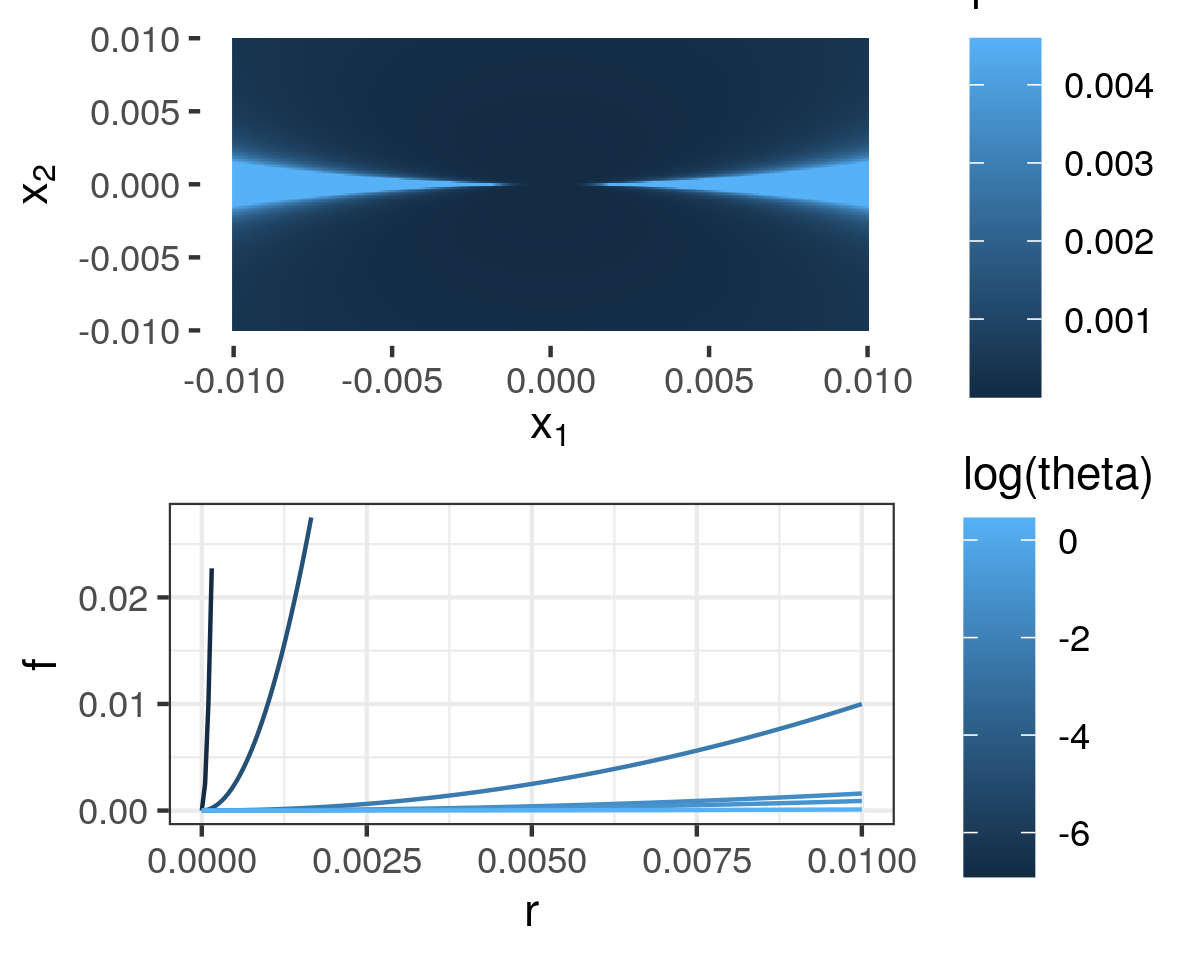
\includegraphics[width=0.980\linewidth,height=0.784\linewidth]{figure/r2_pathological-1} 

}

\caption[A plot of $f(x_1, x_2)$ from \exref{r2_pathological}]{A plot of $f(x_1, x_2)$ from \exref{r2_pathological}.}\label{fig:r2_pathological}
\end{figure}


\end{knitrout}
}


\newcommand{\SimPositivePertFig}{

\begin{knitrout}
\definecolor{shadecolor}{rgb}{0.969, 0.969, 0.969}\color{fgcolor}\begin{figure}[!h]

{\centering 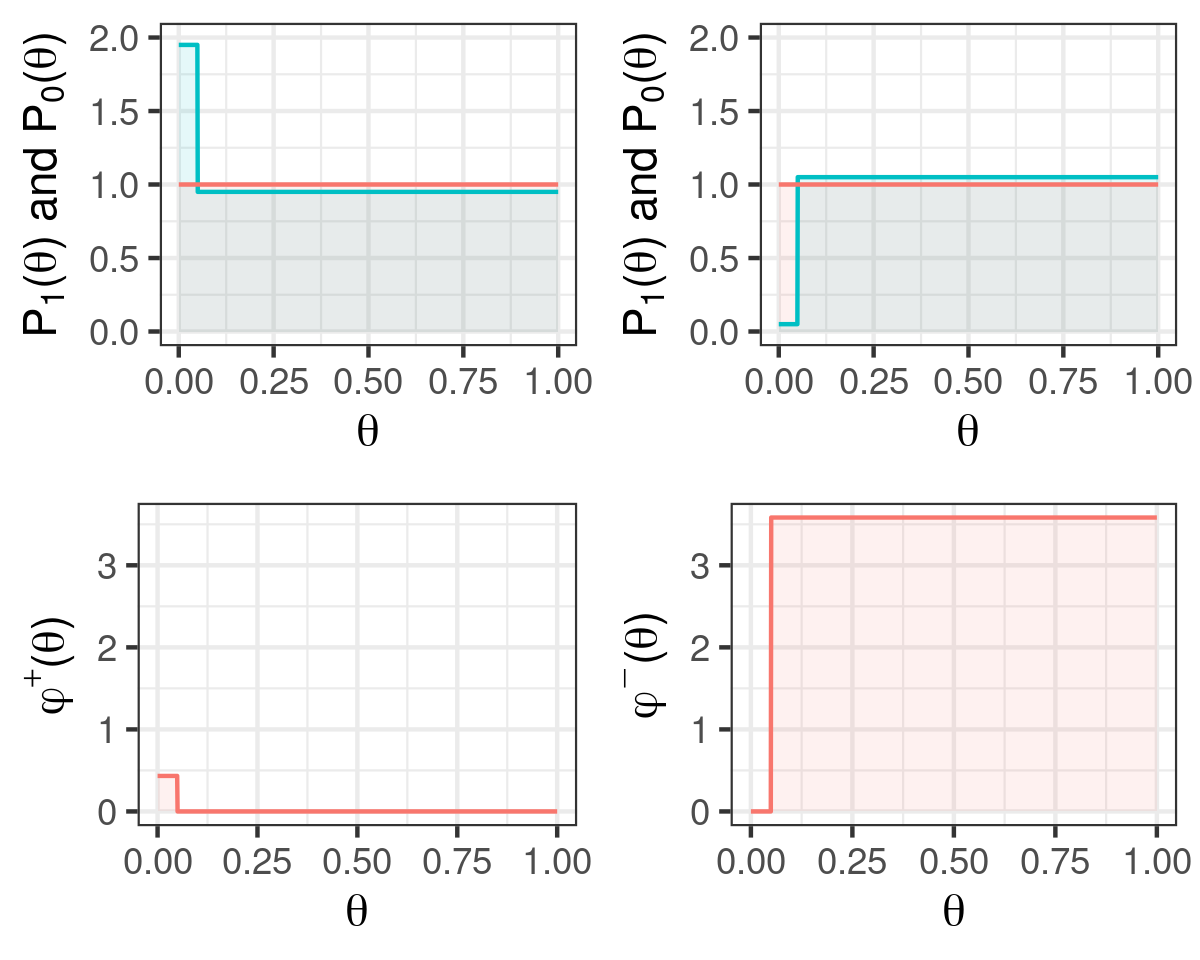
\includegraphics[width=0.980\linewidth,height=0.784\linewidth]{figure/positive_pert-1} 

}

\caption{A plot of the perturbations from \exref{positive_pert_large} with $p=2$ and $\epsilon=0.05$.  Positive $\phi$ can only add mass, so to remove a small amount of mass requires adding mass everywhere else and re-normalizing, resulting in a large perturbation according to $\norm{\cdot}_p$.}\label{fig:positive_pert}
\end{figure}


\end{knitrout}
}


\newcommand{\FunctionPathsFig}{

\begin{knitrout}
\definecolor{shadecolor}{rgb}{0.969, 0.969, 0.969}\color{fgcolor}\begin{figure}[!h]

{\centering 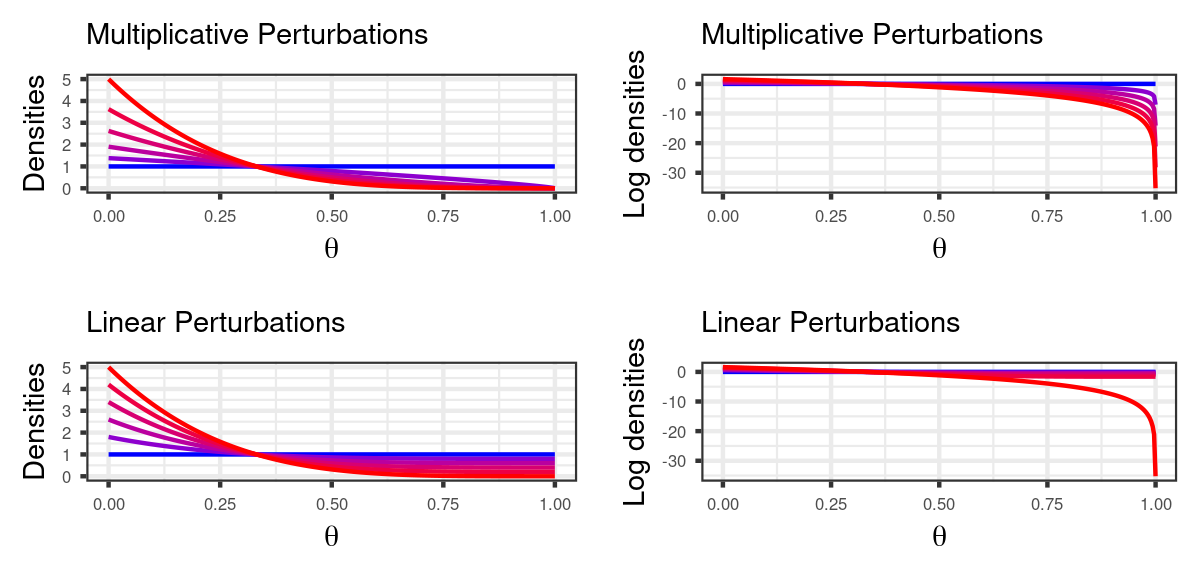
\includegraphics[width=0.980\linewidth,height=0.470\linewidth]{figure/path-1} 

}

\caption[Multiplicative and linear mixture paths between two densities]{Multiplicative and linear mixture paths between two densities.}\label{fig:path}
\end{figure}


\end{knitrout}
}


\newcommand{\FunctionPathsMultFig}{

\begin{knitrout}
\definecolor{shadecolor}{rgb}{0.969, 0.969, 0.969}\color{fgcolor}\begin{figure}[!h]

{\centering 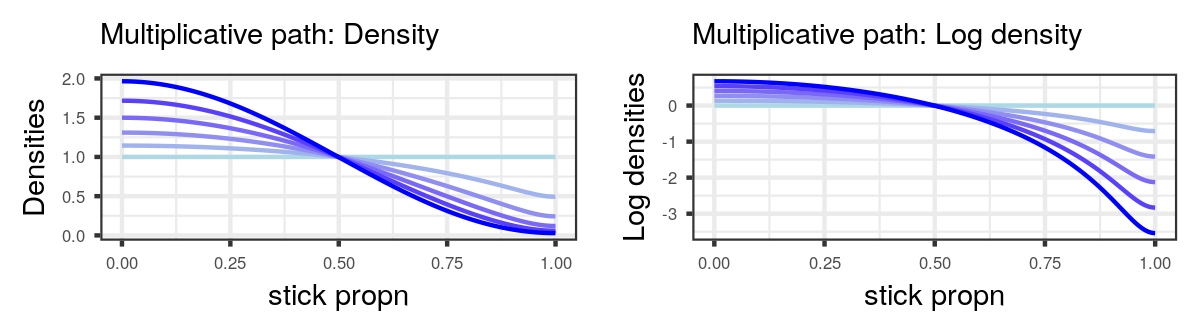
\includegraphics[width=0.980\linewidth,height=0.274\linewidth]{figure/mult_path-1} 

}

\caption[Multiplicative mixture paths between two densities]{Multiplicative mixture paths between two densities.}\label{fig:mult_path}
\end{figure}


\end{knitrout}
}


\newcommand{\FunctionPathsLinFig}{

\begin{knitrout}
\definecolor{shadecolor}{rgb}{0.969, 0.969, 0.969}\color{fgcolor}\begin{figure}[!h]

{\centering 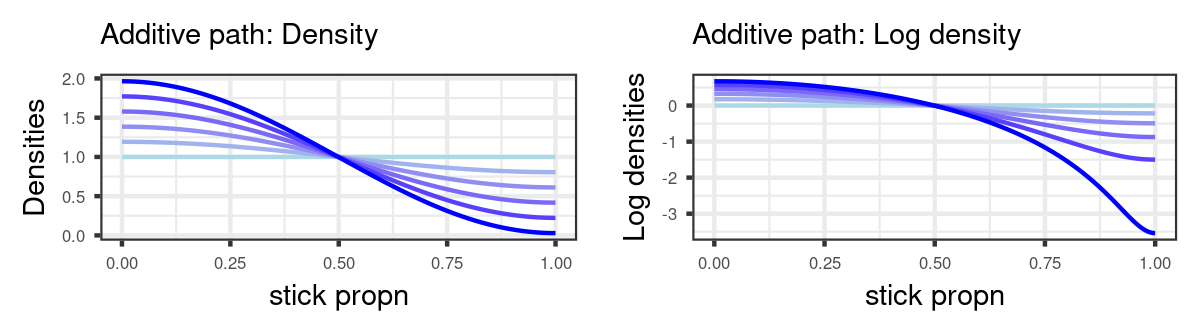
\includegraphics[width=0.980\linewidth,height=0.274\linewidth]{figure/lin_path-1} 

}

\caption[Linear mixture paths between two densities]{Linear mixture paths between two densities.}\label{fig:lin_path}
\end{figure}


\end{knitrout}
}


\newcommand{\FunctionBallFig}{

\begin{knitrout}
\definecolor{shadecolor}{rgb}{0.969, 0.969, 0.969}\color{fgcolor}\begin{figure}[!h]

{\centering 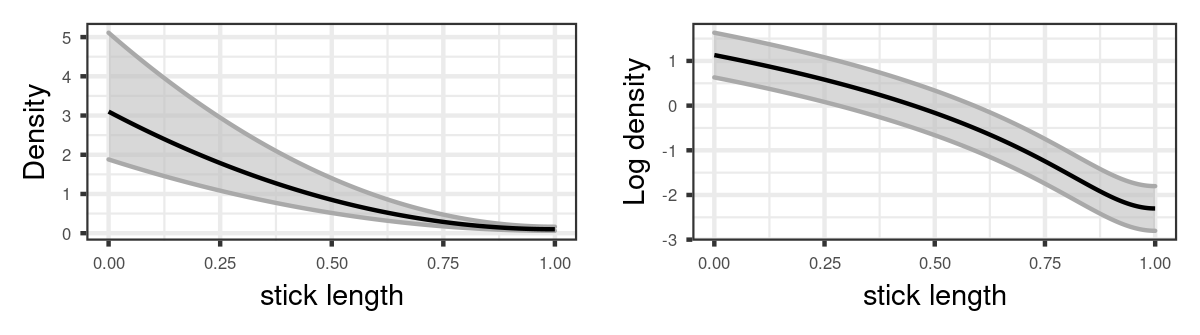
\includegraphics[width=0.980\linewidth,height=0.274\linewidth]{figure/func_ball-1} 

}

\caption[An $\linf{\cdot}$ ball]{An $\linf{\cdot}$ ball.}\label{fig:func_ball}
\end{figure}


\end{knitrout}
}



\title{Evaluating Sensitivity to the Stick Breaking Prior in Bayesian Nonparametrics}

\author{Ryan Giordano \texttt{rgiordan@mit.edu} \\
        \and
        Runjing Liu \texttt{runjing\_liu@berkeley.edu} \\
        \and
        Michael I.\ Jordan \texttt{jordan@cs.berkeley.edu} \\
        \and
        Tamara Broderick \texttt{tbroderick@csail.mit.edu }
        }

\maketitle

\begin{abstract}%   <- trailing '%' for backward compatibility of .sty file

The Dirichlet process has become a mainstay in unsupervised learning tasks
like clustering and topic modeling. Its stick-breaking representation in particular lends itself
to fast approximate posterior inference with variational Bayes. However, choices for the
stick-breaking representation are often made from convenience. For instance, particular
values of the concentration parameter are favored by different applications, and the beta
distribution of the sticks lends itself to conditional conjugacy and closed-form inferential updates.
In many cases, though, different values of the concentration parameter and the underlying stick-breaking
distribution could equally align with prior beliefs. If the major conclusions of our analysis changed under these different reasonable choices, we might worry that our conclusions were driven by arbitrary implementation choices rather than meaningful data trends.
In the present work we demonstrate how to assess the sensitivity of conclusions
to the choice of concentration parameter and stick-breaking distribution. While we focus on perturbations to stick-breaking priors in Bayesian nonparametrics, along the way we develop new theory to support sensitivity analysis more generally for variational Bayes.
\end{abstract}


\section{Introduction}\seclabel{introduction}
Scientists, engineers, and social scientists are often interested in inferring
the number of clusters in a given data set, as well as which observations
cluster together. A common methodology builds on the Dirichlet process
\citep{ferguson:1973:bayesian, sethuraman:1994:constructivedp} from Bayesian
nonparametrics (BNP). BNP methods offer a number of favorable properties. They
allow the number of clusters to grow with the size of the data set; for example,
we might expect to keep discovering new species as we examine more individual
organisms, and we might expect to discover more topics as we read more articles
in a scientific journal. Moreover, BNP methods can be flexibly incorporated into
models of varying complexity. And the Dirichlet process in particular offers a
convenient and well-studied prior on the number and assignment of clusters --
facilitating Bayesian posterior inference and a resulting coherent
quantification of uncertainty.

Nonetheless, Bayesian modeling often involves choices of convenience rather than
pure subjective prior elicitation, and Dirichlet process models are no
exception. For instance, the latent frequencies of clusters -- i.e., the
component proportions -- in a Dirichlet process are generated by recursively
removing beta-distributed fractions of probability mass from the unit interval.
The beta distribution is historically convenient for approximate inference
methods (such as Gibbs sampling) that rely on conditional conjugacy but need not
represent a strong prior belief. Similarly, the Dirichlet process concentration
parameter $\alpha$ may often be chosen based on previous applications rather
than prior belief for the application at hand.
\todo{Cite something (Ryan doesn't have ideas.)}

In general, then, there often exist many possible $\alpha$ values, and many
possible forms of stick-breaking, that might correspond to our prior beliefs.
And these choices can change the results of a data analysis. For instance,
$\alpha$ asymptotically serves as a proportionality constant for the number of
clusters. So the number of clusters at any particular data size may depend
strongly on $\alpha$. If our scientific conclusions varied substantially over
seemingly equivalent prior choices, we might worry that these conclusions are
driven not by our data and meaningful prior beliefs but instead by
somewhat-arbitrary aspects of implementation. It behooves us, then, to check how
sensitive our conclusions are to these choices.

In practice, Bayesian inference requires not just specification of a model and
collection of data but also the use of some posterior approximation. So when we
assess the sensitivity of our conclusions, we should assess the sensitivity of
the full procedure we use in practice. Variational Bayes (VB) is a particularly
popular posterior approximation method for unsupervised learning problems such
as clustering and topic modeling due its fast computation time, increasingly
automated implementations \citep{ranganath:2013:black, kucukelbir:2016:advi},
and avoidance of the label-switching problem exhibited by MCMC
\citep{jasra:2005:mcmclabelswitch}. Therefore, we imagine in what follows that
we have computed the VB approximation for some clustering quantity of interest,
such as number of clusters or cluster co-occurrence.

With a full methodology for clustering in hand, we now can ask how sensitive our
quantity of interest is to the choices of $\alpha$ and the stick-breaking
distributions. One option is to propose a number of potential $\alpha$ values,
compute the variational approximation at each $\alpha$ value, and report our
quantity of interest for each $\alpha$ value. We might similarly assess
sensitivity to the stick-breaking distribution over a range of distributional
choices. There are at least two major issues with this proposal: (1) while VB is
a relatively fast form of approximation Bayesian inference in general, it may
still be prohibitively expensive to have to re-run it many times and (2) it is
unclear how best to choose a collection of $\alpha$ and (especially) the
stick-breaking distribution values -- and how many to choose.

In this work, we circumvent these challenges with a local approximation. VB
posits posterior approximation as an optimization problem. So we show how to
approximate the nonlinear dependence of the VB optimum on prior choices using a
first-order Taylor series expansion. We build on the local robustness tools
developed by \cite{giordano:2018:covariances} for VB and
\cite{gustafson:1996:local} for MCMC. To enable their application to VB for BNP
clustering, we solve a number of open problems; indeed the techniques we
introduce in the current work may be seen to advance sensitivity for VB more
broadly. (1) In particular, we establish that the optimal VB parameters are a
continuously differentiable function of $\alpha$ and the stick-breaking form.
(2) We show that the sensitivity of the VB approximation to functional prior
perturbations takes the form of an integral against a computationally tractable
\textit{influence function} -- and illustrate how the influence function can
provide an interpretable summary of the effect of arbitrary changes to the prior
density. (3) To justify using linear approximations over a ball describing
different stick-breaking densities, we show that our approximation is
\textit{uniformly} good by establishing Fr\'echet differentiability. (4) We how
to efficiently compute our approximation even in high-dimensional problems,
e.g.\ as arise in BNP models. (5) We establish the accuracy, practicality, and
speed of our approximation for a variety of models that use stick-breaking, and
for various quantities of interest in both clustering and topic modeling.



\section{The model and variational approximation}
\seclabel{model}
    \subsection{Discrete Bayesian Nonparametric Model}
    \seclabel{model_bnp}
    A discrete Bayesian nonparametric (BNP) generative model
draws data points $\x_n$ from one of an infinite number of components indexed by
$\k = 1, 2, \ldots \infty$.
Each component is characterized by a vector $\beta_\k \in \betadom \subseteq
\mathbb{R}^{\betadim}$, with $\p(\x_n \vert \beta_\k)$ denoting the
distribution of data arising from  component $\k$.
We model the $\beta_\k$
as arising IID from a known prior, or \textit{base distribution}, denoted
$\pbetaprior(\beta_\k)$, and write
$\beta = (\beta_1, \beta_2, \ldots)$.

Assignment of data point $\n$ to a mixture component is represented by an
(infinite dimensional) vector $\z_\n = (\z_{\n1}, \z_{\n2}, \ldots)$
whose elements $\z_{\n\k} = 1$ for exactly one $\k$ and $0$ otherwise.
With $\z_\n$ defined in this way, we can write
%
\begin{align*}
%
\p(\x_n \vert \z_\n, \beta) =
    \prod_{k=1}^\infty \p(\x_n \vert \beta_\k)^{\z_{\n\k}}.
%
\end{align*}


The prior probabilities of assignments $\z_{\n}$ are generated according
to the following ``stick-breaking" process.
Fix a density $\pstick(\cdot)$, with respect to the
Lebesgue measure, over stick-breaking proportions $\nuk \in (0, 1)$ and
draw $\nuk\iid\pstick(\nuk)$ for $\k=1,2,\ldots\infty$.
Given these stick lengths, construct probabilities using the following formula:
%
\begin{align}\eqlabel{stick_breaking}
%
% \pi_\k := \begin{cases}
% \nuk \prod_{\k' < \k} (1 - \nu_{\k'}) & \textrm{For }k < \infty
%     \textrm{ (all }k\textrm{ when }\infty = \infty\textrm{)}\\
% \prod_{\k' < \k} (1 - \nu_{\k'}). & \textrm{For }k = \infty \\
% \end{cases}
\pi_\k := \nuk \prod_{\k' < \k} (1 - \nu_{\k'}),
%
\end{align}
%
where the empty product is taken to be equal to $1$.
By construction, $\sum_{\k=1}^{\infty} \pi_\k = 1$.
Given the probability vector $\pi := (\pi_1, \pi_2, \ldots)$,
the $\z_\n$ are drawn according to
%
\begin{align*}
%
% \p(\z_{\n\k} = 1 \vert \pi) ={}& \pi_\k \\
% \p(\z_\n \vert \pi) ={}&
%     \ind{\sum_{\k=1}^{\kmax} \z_{\n\k} = 1}
%     \prod_{k=1}^{\kmax} \pi_\k^{\z_{\n\k}}.
\p(\z_\n \vert \pi) ={}&
   \prod_{k=1}^{\infty} \pi_\k^{\z_{\n\k}}.
%
\end{align*}
%
Since $\pi$ is a deterministic function of the stick-breaking proportions
$\nu := (\nu_1, \nu_2, \ldots)$,
we can also write
$\p(\z_\n \vert \nu)$ with no ambiguity.

The stick-breaking distribution $\pstick$ can be thought of as inducing a
a distribution on the vector of probabilities $\pi$. Different
stick-breaking distributions will different favor assignment probabilities, each
with different implied degrees of concentration.
A particularly common choice for
$\pstick(\nuk)$ is the $\mathrm{Beta}(\nuk \vert 1, \alpha)$ distribution,
%
\begin{align*}
%
\mathrm{Beta}(\nuk \vert 1, \alpha) =
    \frac{\Gamma(1 + \alpha) (1 - \nuk)^{\alpha - 1}}
         {\Gamma(\alpha)}.
%
\end{align*}
%
When $\pstick$ is $\mathrm{Beta}(\nuk \vert 1, \alpha)$, the resulting distribution on $\pi$ is known as the
$\textit{GEM distribution}$, and we write $\pi \sim \mathrm{GEM}(\alpha)$.

The GEM distribution is closely related to the Dirichlet process (DP).
Define a measure on $\betadom$ as
\begin{align*}
  \mathcal{M} = \sum_{\k = 1}^\infty \pi_\k\delta_{\beta_\k},
\end{align*}
which places atoms at points $\beta_k$ with weight $\pi_\k$.
When $\pi \sim \mathrm{GEM}(\alpha)$ and
$\beta_\k \iid \pbetaprior(\beta_\k)$, $\mathcal{M}$ is a random measure
is distributed according to Dirichlet process with concentration parameter
$\alpha$ and base measure $\pbetaprior$.

We keep the generic notation $\pstick$ for stick-breaking distributions
because in our sensitivity analysis,
we will consider stick-breaking distributions that are outside the
family of Beta distributions.

In this notation, we can write the joint distribution of
the observed data and latent variables in a basic DP mixture model as:
%
\begin{align}\eqlabel{bnp_model}
%
% \logp(\x, \beta, \z, \nu) ={}&
%     \sum_{n=1}^N \sum_{k=1}^{\kmax}
%         \z_{\n\k} \left(
%             \logp(\x_n \vert \beta_\k) + \log \pi_\k
%         \right) +
% \nonumber \\ {}&
%     \sum_{k=1}^{\kmax} \left(
%         \log \pstick(\nuk) + \logp(\beta_\k)
%     \right).
\logp(\x, \beta, \z, \nu) =&
\sum_{n=1}^N \sum_{k=1}^{\infty}
    \z_{\n\k} \left(
        \logp(\x_n \vert \beta_\k) + \log \pi_\k
    \right)
\nonumber\\
   & +
    \sum_{k=1}^{\infty} \left(
        \log \pstick(\nuk) + \log \pbetaprior(\beta_\k)
    \right).
%
\end{align}
%

%%%%%%%%%%%%%%%%%%%%%%%%%%%%%%%%%%%%%%%%%%%%%%%%%%%%%%%%%%%%%%%%%%%%%%%%%%%%%%%
%%%%%%%%%%%%%%%%%%%%%%%%%%%%%%%%%%%%%%%%%%%%%%%%%%%%%%%%%%%%%%%%%%%%%%%%%%%%%%%
\begin{ex}[Gaussian mixture model]\exlabel{iris_bnp_process}
%
The observations are vectors $\x_\n \in \mathbb{R}^\d$,
and we model each component with a multivariate Gaussian.
In this model, $\beta_\k = (\mu_k, \Lambda_\k)$,
where $\mu_\k \in \mathbb{R}^\d$, $\Lambda_\k$ is a $\d\times\d$ positive
definite information matrix, and
%
\begin{align*}
%
\p(\x_\n \vert \beta_\k) ={}& \normdist{\x_n \vert \mu_\k, \Lambda_\k^{-1}} \\
\logp(\x_\n \vert \beta_\k) ={}&
    -\frac{1}{2}(\x_n - \mu_k)^T \Lambda_\k (\x_n - \mu_k)
    + \frac{1}{2} \log |\Lambda_\k| + \const.\\
    & \constdesc{\beta_\k}
%
\end{align*}
We let $\pbetaprior$ to be the conjugate prior, which in this case is normal-Wishart:
\begin{align*}
  \pbetaprior(\beta_\k) &= \normalwishart{\beta_\k \vert \tau_0, n_0, p_0, V_0}\\
  \log\pbetaprior(\beta_\k) &=
      -\frac{\tau_0}{2}(\mu_\k - \mu_0)^T \Lambda_\k (\mu_\k - \mu_0)\\
      &{} + \frac{n_0 - p_0 - 1}{2} \log |\Lambda_\k| -
      \frac{1}{2} \textrm{Tr}(V_0 \Lambda_\k) + \const,
\end{align*}
where $(\tau_0, n_0, p_0, V_0)$ are fixed prior parameters.

% Below, we fit a
% Gaussian mixture model (GMM) to Fisher's iris data set CITE.
% Each observation is an iris flower with
% four measurements:
% sepal length, sepal width, petal length, and petal width.
% The components in this model can be interpreted as latent iris species;
% the inferential goal is to estimate $\z_\n$ and assign each
% observed flower to a latent species.

% For the iris data, we might imagine that each cluster corresponds to a different
% species with a different distribution of flower dimensions.  The BNP model
% implies that there are a potentially infinite number of differet iris species
% that we might observe.  Then $\z_{\n\k} = 1$ would mean that observation $\n$
% was a member of species $\k$, and $\sum_{k=1}^\kmax \ind{ \sum_{n=1}^{N}
% \z_{\n\k} > 1}$ is the number of distinct species observed in our particular
% dataset.
%
\end{ex}

We started with a Gaussian mixture model (GMM)
because it conforms cleanly to the
generative process culminating in \eqref{bnp_model}.
In \secref{results_iris}, we fit a GMM to Fisher's iris data set
\citep{anderson:1936:iris, fisher:1936:iris} and
cluster irises into latent species based on morphological measurements.
The next two examples, which we will apply to real data sets
(\secref{results_mice, results_structure}),
require more careful modeling considerations,
and we adjust the factorization in \eqref{bnp_model} to suit our purposes.

%%%%%%%%%%%%%%%%%%%%%%%%%%%%%%%%%%%%%%%%%%%%%%%%%%%%%%%%%%%%%%%%%%%%%%%%%%%%%%%
%%%%%%%%%%%%%%%%%%%%%%%%%%%%%%%%%%%%%%%%%%%%%%%%%%%%%%%%%%%%%%%%%%%%%%%%%%%%%%%

\begin{ex}[Regression mixture model]\exlabel{mice_bnp_process}

We cluster time-course gene expression data.
An observation $\x_\n\in\mathbb{R}^\ntimepoints$ is a vector of
expression levels at $\ntimepoints$
time points.
Let $\regmatrix$ be an $\ntimepoints \times \d$ regressor matrix;
in our case, we will use a cubic B-spline, so the $ij$-th entry of $\regmatrix$
is the $j$-th B-spline basis vector evaluated at the
$i$-th time point (\secref{results_mice}).

Each component is characterized by a vector of regression coefficients
$\mu_\k$ and a variance $\tau^{-1}_\k$, so
in this model, $\beta_k = (\mu_\k, \tau_\k)$.
The distribution of the data arising from component $k$ is
\begin{align*}
\p(\x_\n | \beta_\k, \b_\n) =
\normdist{\x_\n | \regmatrix\mu_\k + \b_\n,
\tau_\k^{-1}I_{\ntimepoints \times \ntimepoints}},
\end{align*}
%
where $\b_{n}$ is a gene-specific additive offset.
We include the additive offset because we
are interested in clustering gene expressions based on their patterns over time,
not their absolute level.

The joint distribution can be written in the same form as~\eqref{bnp_model},
except that the conditional data likelihood now depends on $\b_\n$ in addition to $\beta_\k$,
and we include an additional prior term for $\b_\n$. 
% \begin{align*}
% \logp(\x, \beta, \z, \nu, \b) =&
%     \sum_{n=1}^N \sum_{k=1}^{\infty}
%         \z_{\n\k} \left(
%             \logp(\x_n \vert \beta_\k, \b_n) + \log \pshift(\b_n) + \log \pi_\k
%         \right)  \\
%     &{} + \sum_{k=1}^{\infty} \left(
%         \log \pstick(\nuk) + \log \pbetaprior(\beta_\k)
%     \right).
% \end{align*}
%
\end{ex}

%%%%%%%%%%%%%%%%%%%%%%%%%%%%%%%%%%%%%%%%%%%%%%%%%%%%%%%%%%%%%%%%%%%%%%%%%%%%%%%
%%%%%%%%%%%%%%%%%%%%%%%%%%%%%%%%%%%%%%%%%%%%%%%%%%%%%%%%%%%%%%%%%%%%%%%%%%%%%%%

Our last example is a Bayesian topic model applied to genetic data.
Genotypes at genetic markers take the place of
words in a document; in lieu of inferring ``topics," we infer latent populations.

\begin{ex}[A topic model for population structure]\exlabel{structure_bnp_process}

We consider genetic data where the
data set consists of $\nindiv$ individuals genotyped at $\nloci$ loci.
For diploid organisms, there are two observations at each loci, one at each chromosome.
Let $\x_{\n\l\i}\in\{1, \ldots, J_\l\}$ be the observed genotype for
individual $\n$ at locus $\l$ and chromosome $\i$;
$J_\l$ is the number of possible genotypes at locus $\l$.
For example, if the measurements are single nucleotides (A, T, C or G)
then $J_\l = 4$ for all $\l$.

A latent population is characterized by the collection
$\beta_k = (\latentpop_{\k1}, \ldots, \latentpop_{\k\nloci})$ where
$\latentpop_{\k\l}\in\Delta^{J_\l - 1}$ are the latent frequencies for the $J_l$
possible genotypes at locus $\l$.
Let $\z_{\n\l\i}$ be the assigment of observation $\x_{\n\l\i}$ to a latent population.
Note that for a given individual $\n$,
different loci, and even different chromosomes at a given locus,
may be assigned to different populations.
The distribution of $\x_{\n\l\i}\in\{1, \ldots, J_\l\}$ arising from population $\k$ is
\begin{align*}
\p(\x_{\n\l\i} \vert \latentpop_{\k}) =
\categoricaldist{\x_{\n\l\i}\vert \latentpop_{\k\l}}.
\end{align*}


Unlike the previous models, we now have a stick-breaking process for each individual.
Draw sticks
\begin{align*}
\nu_{\n\k} \iid \pstick(\nu_{\n\k}) \quad \forall \n = 1, \ldots, \nindiv; \k = 1, 2, \ldots \infty.
\end{align*}
The prior assignment probabilities
$\latentadmix_{\n} = (\latentadmix_{\n1}, \latentadmix_{\n2}, \ldots)$
are formed by the usual stick-breaking construction,
%
\begin{align*}
\latentadmix_{\n\k} = \nu_{\n\k} \prod_{\k' < \k} (1 - \nu_{\n\k'}).,
\end{align*}
%
from which the population assignment $\z_{\n\l\i}$ is drawn according to the
usual multinomial distribution
%
\begin{align*}
p(\z_{\n\l\i} | \latentadmix_\n) = \prod_{k=1}^{\infty} \latentadmix_{\n\k}^{\z_{\n\l\i\k}}.
\end{align*}
%
In this genetics application,
we call $\latentadmix_{\n}$ the
\textit{admixture} of individual $\n$.


The joint log-likelihood decomposes as
\begin{align*}
\logp(\x, \latentpop, \z, \nu) &=
\sum_{\n=1}^\nindiv \sum_{\l=1}^\nloci \sum_{i = 1}^2 \sum_{\k=1}^{\infty}
        \z_{\n\l\i\k} \left(
            \logp(\x_{\n\l\i} \vert \latentpop_{\k}) + \log \pi_{\n\k}
        \right)
\nonumber\\&
    \quad +
    \sum_{\n=1}^\nindiv \sum_{k=1}^{\infty} \log \pstick(\nu_{\n\k})
    + \sum_{k=1}^{\infty} \log \pbetaprior(\latentpop_{\k}).
\end{align*}

This model is identical to STRUCTURE,
a model proposed in \citet{pritchard:2000:structure, raj:2014:faststructure},
except that we replace the Dirichlet prior in STRUCTURE
with an infinite stick-breaking process.
The result is a model similar to a heirchical Dirichlet process for topic modeling,
\citep{teh:2006:hdp},
but without the top-level Dirichlet process.
%
\end{ex}


%%%%%%%%%%%%%%%%%%%%%%%%%%%%%%%%%%%%%%%%%%%%%%%%%%%%%%%%%%%%%%%%%%%%%%%%%%%%%%%


    \subsection{Variational Approximation}
    \seclabel{model_vb}
    There are two practical problems with forming the posterior
$p(\theta, \z \vert \x)$ based on the joint distribution given in
\eqref{bnp_model}.  First, there are an infinite number of parameters,
and second, the posterior is intractable.  In this section, we describe
how we circumvent these difficulties using a truncated variational Bayes
approximation (CITE).

In practice, forming a posterior based on \eqref{bnp_model} with $\kmax =
\infty$ can be challenging.  In the present paper, we will follow CITE BLEI and
use a ``truncated model'' where $\kmax$ is large but finite. We ensure that a
large proportion of the clusters are unoccupied with high posterior probability,
in which case the truncation approxes the fully nonparametric case with $\kmax =
\infty$ (CITE HUGGINS).  Under this truncation, the final cluster (indexed by
$\kmax$) can be thought of as capturing the contribution from the tail of
clusters that are not explicitly represented in the truncated model.

Under the truncation, our model differs formally from standard finite mixture
models principally in our usage of the stick breaking prior rather than, say,
the Dirichlet prior.  Using the stick breaking prior is appealing due to its
connection to the fully nonparametric model.  Additionally, the stick breaking
prior deals more gracefully than the Dirichlet prior with a large $\kmax$.  For
example, unless the Dirichlet parameter scales as $1 / \kmax$, then Dirichlet
priors strongly favor a large number of  distinct clusters as $\kmax$ grows
larger \citep[Problem 3]{stanford:2014:bnphw}.

Second, even with finite $\kmax$, the posterior for \eqref{bnp_model} is
intractable, so we again follow CITE BLEI and emply a mean field variational
approximation.  Let $\zeta := (\theta, \z, \nu)$ denote the full vector of
posterior parameters.  We form our variational approximation by specifying a
family of approximating distributions of the form $\q(\zeta \vert \eta)$,
parameterized by a finite-dimensional $\eta \in \etadom \subseteq
\mathbb{R}^{\etadim}$, such that $\q(\zeta \vert \eta)$ is absolutely continuous
with respect to the prior $p(\zeta)$ for all $\eta \in \etadom$.  As we discuss
below, we will choose $\q(\zeta \vert \eta)$ so that we can easily compute or
approximation expectations with respect to $\q(\zeta \vert \eta)$, and so that
$\q(\zeta \vert \eta)$ has tractable entropy as a function of $\eta$.

Given our family of variational approximations, we wish to find the member of
the family that is closest to the posterior $p(\zeta \vert \x)$ in
Kullback-Leibler (KL) divergence:
%
\begin{align}\eqlabel{vb_optimization}
%
\etaopt :={}&
    \argmin_{\eta \in \etadom}
        \KL{\q(\zeta \vert \eta) || p(\zeta \vert \x)} \mathwhere \\
\KL{\q(\zeta \vert \eta) || p(\theta \vert \x)}
={}&    \expect{\q(\zeta \vert \eta)}{
        \log \q(\zeta \vert \eta) - \logp(\x \vert \zeta) -
        \logp(\zeta)} + \logp(\x). \nonumber
%
\end{align}
%
Due to properties of $\q(\zeta \vert \eta)$ or as given in \eqref{bnp_model},
all the terms in $\KL{\q(\zeta \vert \eta) || p(\theta \vert \x)}$ are tractable
except for $\logp(\x)$.  However, $\logp(\x)$ does not depend on $\eta$, and
so can be negelcted in the optimziation.

We will use mean-field variational approximating families of the following form:
%
\begin{align}\eqlabel{vb_mf}
%
\q(\zeta \vert \eta) =
    \left( \prod_{\k=1}^{\kmax - 1} \q(\nu_\k \vert \eta) \right)
    \left( \prod_{\k=1}^{\kmax} \q(\theta_\k \vert \eta) \right)
    \left( \prod_{\n=1}^{\N} \q(\z_{\n} \vert \eta) \right).
%
\end{align}
%
Under this parameterization, the vector $\eta$ will partition into parameters
governing $\nu$, $\theta$, and $\z$.  Let the VB parameters governing a
particular parameter vector be denoted with a subscript: for example, $\q(\theta
\vert \eta) = \q(\theta \vert \etatheta)$, $\q(\z_\n \vert \eta) = \q(\z \vert
\eta_{\z_{\n}})$, and so on.

For $\z$ and $\theta$, in the present work, we will be always able to take
advantage of conditional conjugacy.  Specifically, we will take $\q(\z_{\n}
\vert \eta)$ to be multinomial with a single observation, matching $p(\z_{\n}
\vert \x, \theta, \nu)$, and we will take $\q(\theta_\k \vert \eta)$, matching
the distribution of $p(\theta_{\k} \vert \x, \z, \nu)$.

%%%%%%%%%%%%%%%%%%%%%%%%%%%%%%%%%%%%%%%%%%%%%%%%%%%%%%%%%%%%%%%%%%%%%%%%%%%%%%%
%%%%%%%%%%%%%%%%%%%%%%%%%%%%%%%%%%%%%%%%%%%%%%%%%%%%%%%%%%%%%%%%%%%%%%%%%%%%%%%

\begin{ex}[VB approximation for $\theta_\k$]
%
Recall for the iris dataset we used $p(\x_\n \vert \theta_\k) = \norm{\x_n \vert
\mu_\k, \Sigma_\k}$, with $\theta_\k = (\mu_\k, \Sigma_\k)$.  So,
up to a constant not depending on $\eta$,
%
\begin{align*}
%
\MoveEqLeft
\expect{\q(\theta_\k \vert \eta)}{\logp(\x_\n \vert \theta_\k)} =\\
&
\expect{\q(\theta_\k \vert \eta)}{
-\frac{1}{2}(\x_n - \mu_k)^T \Sigma_\k^{-1} (\x_n - \mu_k)} +
+\frac{1}{2} \expect{\q(\theta_\k \vert \eta)}{\log |\Sigma_\k^{-1}|}.
%
\end{align*}
%
By taking $\q(\theta_\k \vert \eta) = \wishart{\Sigma_\k^{-1} \vert \eta}
\norm{\mu_\k \vert \eta}$, the expectations in the preceding display have closed
form expressions as functions of $\eta$, as does the entropy
$\expect{\q(\theta_\k \vert \eta)}{\log \q(\theta_\k \vert \eta)}$.
%
\end{ex}

%%%%%%%%%%%%%%%%%%%%%%%%%%%%%%%%%%%%%%%%%%%%%%%%%%%%%%%%%%%%%%%%%%%%%%%%%%%%%%%


%%%%%%%%%%%%%%%%%%%%%%%%%%%%%%%%%%%%%%%%%%%%%%%%%%%%%%%%%%%%%%%%%%%%%%%%%%%%%%%
%%%%%%%%%%%%%%%%%%%%%%%%%%%%%%%%%%%%%%%%%%%%%%%%%%%%%%%%%%%%%%%%%%%%%%%%%%%%%%%

\begin{ex}[VB approximation for $\z_\n$]\exlabel{qz_form}
%
From \eqref{bnp_model}, we have in general that
%
\begin{align*}
%
\logp(\z_n \vert \x, \theta, \nu) ={}&
\sum_{k=1}^{\kmax}
    \z_{\n\k} \left(
        \logp(\x_n \vert \theta_\k) + \log \pi_\k
    \right) + \const & \constdesc{\z_\n}.
%
\end{align*}
%
So, from the mean field assumption of \eqref{vb_mf},
%
\begin{align*}
%
\expect{\q(\zeta \vert \eta)}{\logp(\z_n \vert \x, \theta, \nu)} ={}&
\sum_{k=1}^{\kmax}
    \expect{\q(\z_\n \vert \eta)}{\z_{\n\k}}
    \expect{\q(\theta, \nu \vert \eta)}
           {\logp(\x_n \vert \theta_\k) + \log \pi_\k}.
%
\end{align*}
%
When $\q(\z_\n \vert \eta)$ is multinomial, the needed expectation
$\expect{\q(\z_\n \vert \eta)}{\z_{\n\k}}$ has a closed form, as does the
entropy,
%
\begin{align*}
%
\expect{\q(\z_\n \vert \eta)}{\log \q(\z_\n \vert \eta)} ={}&
    - \sum_{\k=1}^{\kmax}
        \expect{\q(\z_\n \vert \eta)}{\z_{\n\k}}
        \log \left( \expect{\q(\z_\n \vert \eta)}{\z_{\n\k}} \right).
%
\end{align*}
%
Additionally, given $\etatheta$ and $\etanu$, the optimal
variational distribution $\q(\z_\n \vert \etaoptz)$ has a closed form, with
%
\begin{align*}
%
\expect{\q(\z_\n \vert \etaopt)}{\z_{\n\k}} ={}&
\frac{
    \expect{\q(\theta, \nu \vert \eta)}
           {\logp(\x_n \vert \theta_\k) + \log \pi_\k}
}{
    \sum_{\k'=1}^{\kmax}
    \expect{\q(\theta, \nu \vert \eta)}
           {\logp(\x_n \vert \theta_{\k'}) + \log \pi_{\k'}}
}.
%
\end{align*}
%
This fact will be helpful later in \secref{local_sensitivity}.
%
\end{ex}

%%%%%%%%%%%%%%%%%%%%%%%%%%%%%%%%%%%%%%%%%%%%%%%%%%%%%%%%%%%%%%%%%%%%%%%%%%%%%%%

For our sensitivity analysis in \secref{local_sensitivity}, we will require
$\etaopt$ to be interior to $\etadom$.  Consequently, we will choose
unconstrained representations of the needed distributions or parameters.

%%%%%%%%%%%%%%%%%%%%%%%%%%%%%%%%%%%%%%%%%%%%%%%%%%%%%%%%%%%%%%%%%%%%%%%%%%%%%%%
%%%%%%%%%%%%%%%%%%%%%%%%%%%%%%%%%%%%%%%%%%%%%%%%%%%%%%%%%%%%%%%%%%%%%%%%%%%%%%%

%[Unconstrained representation for $\etaz$]
\begin{ex}\exlabel{qz_unconstrained}
%
The multinomial approximating distribution $\q(\z_\n \vert \etaz)$ as given in
\exref{qz_form} is fully specified by the expectations $\expect{\q(\z_\n \vert
\etaopt)}{\z_{\n\k}} \in (0, 1)$.  But these expectations have only $\kmax -1$
degrees of freedom since, for any valid $\q(\z_\n \vert \etaz)$,
$\sum_{\k=1}^\kmax \expect{\q(\z_\n \vert \etaopt)}{\z_{\n\k}} = 1$, and so the
optimal values for $\expect{\q(\z_\n \vert \etaopt)}{\z_{\n\k}}$ cannot be
interior to $(0,1)^\kmax$.  Consequently we parameterize
$\q(\z_\n \vert \etaz)$ using the unconstrained parameters $\rho_{\n\k}$,
for $\k=1,\ldots,\kmax - 1$, where
%
\begin{align*}
%
\expect{\q(\z_\n \vert \etaz)}{\z_{\n\k}} =
\begin{cases}
    \frac{\exp(\rho_{\n\k})}{1 + \sum_{\k'=1}^{\kmax - 1}\exp(\rho_{\n\k})}
    & \mathrm{ when }\quad\k < \kmax \\
    \frac{1}{1 + \sum_{\k'=1}^{\kmax - 1}\exp(\rho_{\n\k})}
    & \mathrm{ when }\quad\k = \kmax.
\end{cases}
%
\end{align*}
%
We thus take $\etaz = (\rho_{11}, \ldots \rho_{1(\kmax - 1)}, \ldots,
\rho_{\n(\kmax - 1)})$ to be the stacked vector of $\rho_{\n\k}$.
%
\end{ex}
%%%%%%%%%%%%%%%%%%%%%%%%%%%%%%%%%%%%%%%%%%%%%%%%%%%%%%%%%%%%%%%%%%%%%%%%%%%%%%%



For the stick-breaking distributions $\q(\nu_\k \vert \eta)$ we will need to do
something more complicated, since we wish to accomodate generic stick breaking
distributions.  From \eqref{bnp_model} we see that, up to a constant not
depending on $\nu_\k$,
%
\begin{align}\eqlabel{stick_log_post}
%
\log \pi_\k ={}&
    \log \nu_\k + \sum_{\k' < \k} \log (1 - \nu_\k) \nonumber \\
\logp(\nu_{\k} \vert \x, \theta, \z) ={}&
    \left(\sum_{\n=1}^\N \z_{\n\k'}\right) \log \nu_\k +
    \left( \sum_{\k' > \k} \sum_{\n=1}^\N \z_{\n\k'} \right) \log (1 - \nu_\k) +
    \log \pstick(\nu_\k).
%
\end{align}
%
When $\pstick(\cdot) = \mathrm{Beta}(\cdot | 1, \alpha)$, then, up to a constant
not depending on $\nu_\k$, $\log \pstick(\nu_\k) = (\alpha - 1) \log (1 -
\nu_\k)$, so $\logp(\nu_{\k} \vert \x, \theta, \z)$ is proportional to the
sufficient statistics $\log \nu_\k$ and $\log(1 - \nu_\k)$ and so in the
Beta family.  However, for a generic $\pstick(\cdot)$, the posterior
$p(\nu_{\k} \vert \x, \theta, \z)$ does not have a standard form.

In order to optimize the variational objective \eqref{vb_optimization} we see
from \eqref{stick_log_post} that we need to evaluate or approximate expectations
of the form
%
\begin{align*}
%
\expect{\q(\nu_\k \vert \eta)}{\log \nu_\k}
\textrm{,}\quad
\expect{\q(\nu_\k \vert \eta)}{\log (1 - \nu_\k)}
\textrm{,}\quad\textrm{and}\quad
\expect{\q(\nu_\k \vert \eta)}{\log \pstick(\nu_\k)}.
%
\end{align*}

Each of the expecations are univariate integrals, and so can be efficiently
approximated numerically.  A particularly easy way to do so is with
Gauss-Hermite (GH) quadrature, as we now describe.

First, define a version of $\nu_\k$ that is not constrained to $(0,1)$:
%
\begin{align*}
%
\lnu_\k :={} \log \left( \frac{\nu_\k}{1 - \nu_\k} \right)
\quad\Leftrightarrow\quad
\nu_\k :={} \frac{\exp(\lnu_\k)}{1 + \exp(\lnu_\k)}.
%\fracat{d \lnu_\k}{ d\nu_\k}{\nu_\k} ={}&
%     \frac{1-\nu_\k}{\nu_\k}
%     \left(\frac{1}{1 - \nu_\k} + \frac{\nu_\k}{(1 - \nu_\k)^2} \right)
% \\={}& \frac{1}{\nu_\k} + \frac{1}{1 - \nu_\k}
% \\={}&
%\frac{1}{\nu_\k (1 - \nu_\k)}.
%
\end{align*}
%
We wish to let $\lnu_\k$ be distributed normally under the variational
distribution.  Let $\lnumean_\k$ and $\lnusd_\k$ be entries of the parameter
vector $\eta$, and write
%
\begin{align*}
%
\q(\lnu_\k \vert \eta) ={}& \norm{\lnu_\k \vert \lnumean_\k, \lnusd_\k}
\Rightarrow \\
\q(\nu_\k \vert \eta) ={}&
    \norm{\log \left( \frac{\nu_\k}{1 - \nu_\k} \right)
        \vert \lnumean_\k, \lnusd_\k}
    \left|\fracat{d \lnu_\k}{ d\nu_\k}{\nu_\k}\right|
\\={}&
\norm{\log \left( \frac{\nu_\k}{1 - \nu_\k} \right)
        \vert \lnumean_\k, \lnusd_\k}
    \left|\frac{1}{\nu_\k (1 - \nu_\k)}\right|.
%
\end{align*}
%
Given this, we can approximate expectations of smooth functions
$f(\nu_\k)$ using GH quadrature with $\ngh$ knots,
located at $\xi_g$, weighted by $\omega_g$:
%
\begin{align}\eqlabel{gh_integral}
%
\expect{\q(\nu_\k \vert \eta)}{f(\nu_\k)} ={}&
\expect{\q(\lnu_\k \vert \eta)}
       {f\left(\frac{\exp(\lnu_\k)}{1 + \exp(\lnu_\k)}\right)}
\nonumber\\\approx{}&
    \sum_{g=1}^{\ngh} \omega_g f\left(\lnusd_\k \xi_{g} + \lnumean_\k\right)
 \nonumber\\=:{}&
\expecthat{\q(\nu_\k \vert \eta)}{f(\nu_\k)}.
%
\end{align}
%
Conveniently, $\expecthat{\q(\nu_\k \vert \eta)}{f(\nu_\k)}$ is a differentiable
function of $\lnumean_\k$ and $\lnusd_\k$, and so also of $\eta$.  (This
technique is similar to the ``reparameterization trick,'' only using
GH points rather than standard normal draws.)


    % \subsection{Robustness and the Taylor series approximation}
    % \seclabel{model_taylor}
    % 

%%%%%%%%%%%%%%%%%%%%%%%%%%%%%%%%%%%%%%%%%%%%%%%%%%%%%%%%%%%%%%%%%%%%%%%%%%%%%%%

\subsection{Choices for $\pstick$}

Typically, many different choices for $\pstick$ may be {\em a priori}
reasonable.  A particularly common choice for $\pstick$ is the
$\mathrm{Beta}(\nuk \vert 1, \alpha)$ density, which we write as
%
\begin{align*}
%
\pstick(\nuk \vert \alpha) :=
\mathrm{Beta}(\nuk \vert 1, \alpha) =
    \frac{\Gamma(1 + \alpha) (1 - \nuk)^{\alpha - 1}}
         {\Gamma(\alpha)},
%
\end{align*}
%
When $\pstick$ is $\mathrm{Beta}(\nuk \vert 1, \alpha)$, the resulting
distribution on $\pi$ is known as the $\textit{GEM distribution}$, and we write
$\pi \sim \mathrm{GEM}(\alpha)$.
%
The GEM distribution is closely related to the Dirichlet process (DP).
Define a measure on $\betadom$ as
%
\begin{align*}
  \mathcal{M} = \sum_{\k = 1}^\infty \pi_\k\delta_{\beta_\k},
\end{align*}
%
which places atoms at points $\beta_k$ with weight $\pi_\k$. When $\pi \sim
\mathrm{GEM}(\alpha)$ and $\beta_\k \iid \pbetaprior(\beta_\k)$, $\mathcal{M}$
is a random measure is distributed according to Dirichlet process with
concentration parameter $\alpha$ and base measure $\pbetaprior$
\citep{ferguson:1973:bayesian, sethuraman:1994:constructivedp}.

Typically, the concentration parameter $\alpha$ is not known in advance.
Rather, $\alpha$ may {\em a priori} plausibly lie within some reasonable range.
Since the prior $\pstick(\nuk \vert \alpha)$ depends on $\alpha$, the posterior
the posterior expectation $\expect{\p(\z \vert \x, \alpha)}{\nclusters_0(\z)}$
depends on $\alpha$ as well.  If $\expect{\p(\z \vert \x,
\alpha)}{\nclusters_0(\z)}$ varies meaningfully as $\alpha$ varies over its
plausible values, then the quantity of interest $\expect{\p(\z \vert \x,
\alpha)}{\nclusters_0(\z)}$ is not robust to the choice of $\alpha$.

In practice, one chooses some ``base value,'' $\alpha_0$, and runs a
computationally expensive posterior approximation procedure such variational
Bayes (VB), giving an approximate value for $\expect{\p(\z \vert \x,
\alpha_0)}{\nclusters_0(\z)}$.


More generally, there may be no {\em a priori} reason to believe that $\pstick$
lies in the Beta family at all (other than computational convenience). By
$\pbase$ and $\palt$ denote two candidate stick-breaking densities, we can
. Suppose that
parameterizing one-dimensional paths in the space of prior densities.  Let
$\pbase$


%
%
%
%
% Even if one is willing to restrict However, there is typically no {\em a priori}
% reason to assume that $\pi \sim \mathrm{GEM}(\alpha)$ is a realistic summary of
% our prior beliefs for any particular $\alpha$.
%
%
% We keep the generic notation $\pstick$ for stick-breaking distributions because
% in our sensitivity analysis, we will consider stick-breaking distributions that
% are outside the family of Beta distributions.



\section{Differentiability of the VB optimum}
\seclabel{local_sensitivity}
Our goal is to approximate the dependence of the optimal VB parameters on the
prior using a Taylor series, which requires that the optimal VB parameters must
be continuously differentiable as a function of the prior specification. In this
section we state general conditions under which VB optima, as defined by
\eqref{vb_optimization}, are differentiable functions of both parametric and
nonparametric prior perturbations.

We will state our conditions and results in terms of a generic VB approximation
and prior perturbation, which we now articulate in  \defref{prior_t}. The
desired results for the BNP model will follow as special cases of these general
results.

%%%%%%%%%%%%%%%%%%%%%%%%%%%%%%%%%%%%%%%%%%%%%%%%%%%%%%%%%%%%%%%%%%%%%%%%%%%
%%%%%%%%%%%%%%%%%%%%%%%%%%%%%%%%%%%%%%%%%%%%%%%%%%%%%%%%%%%%%%%%%%%%%%%%%%%%
\begin{defn}\deflabel{prior_t}
%
For some parameter $\theta \in \thetadom \subseteq \mathbb{R}^{\thetadim}$, let
$\p(\theta \vert \t)$ denote a class of probability densities relative to
a sigma-finite measure $\mu$, defined for $\t$ in an open set $\ball_\t
\subseteq \mathbb{R}$ containing $0$.  Let $\q(\theta \vert \eta)$ be a
family of approximating densities, also defined relative to $\mu$.

Let the variational objective factorize as
%
\begin{align}
%
\KL{\eta, \t} :={}&
    \KL{\eta} -
    \expect{\q(\theta \vert \eta)}
       {\left(\log \p(\theta \vert \t) - \log \p(\theta \vert \t=0)\right)}           \eqlabel{perturbed_objective}\\
\etaopt(\t) :={}& \argmin_{\eta \in \etadom} \KL{\eta, \t}.
    \eqlabel{perturbed_optimum}
%
\end{align}
%
Let $\etaopt$ with no argument refer to $\etaopt(0)$, the minimizer
of $\KL{\eta}$.
%
\end{defn}
%%%%%%%%%%%%%%%%%%%%%%%%%%%%%%%%%%%%%%%%%%%%%%%%%%%%%%%%%%%%%%%%%%%%%%%%%%%%

The decomposition \eqref{perturbed_objective} is always possible, in the sense
that one could always take $\theta = \zeta$ and $\KL{\eta} = 0$.  We decompose
the objective in this way in order to state strict regularity assumptions only
on the part of the KL divergence that is being perturbed.  Indeed, we will
require little from the $\KL{\eta}$ part of the decomposition other than that it
can be differentiated and optimized.

By identifying $\t$ with some hyperparameter (e.g. the concentration parameter,
as in \exref{alpha_perturbation} below), we can use \defref{prior_t} to study
parametric perturbations.  Furthermore, by parameterizing a path through the
space of general densities, \defref{prior_t} will allow us to study
nonparametric perturbations (e.g. \exref{gem_mult_perturbation} below and the
detailed analysis of \secrangeref{diffable_nonparametric}{diffable_lp}).  We
can thus study VB prior robustness in general by studying problems of the
form \defref{prior_t}.

%%%%%%%%%%%%%%%%%%%%%%%%%%%%%%%%%%%%%%%%%%%%%%%%%%%%%%%%%%%%%%%%%%%%%%%%%%%%%%%%
%%%%%%%%%%%%%%%%%%%%%%%%%%%%%%%%%%%%%%%%%%%%%%%%%%%%%%%%%%%%%%%%%%%%%%%%%%%%%%%%
\begin{ex}\exlabel{alpha_perturbation}
%
For the BNP model with the $\gem$ prior, take $\theta = (\nu_1, \ldots,
\nu_{\kmax-1})$, and take $\mu$ to be the Lebesgue measure on $[0,1]^{\kmax-1}$.
Let $\alpha_0$ be some initial value of the concentration parameter, and
let $\t$ be $\alpha - \alpha_0$, so that deviations of $\t$ away from
$0$ represent deviations of $\alpha$ away from $\alpha_0$.

Expanding the KL divergence in \eqref{kl_def}, we see that the prior
$\p(\nuk \vert \alpha)$ enters the VB objective in a term of the form
$\sum_{\k=1}^\infty \expect{\q(\nuk \vert \eta)}{\log \p(\nuk \vert \alpha)}$.
Adding and subtracting the this term evaluated at $\alpha_0$ gives
%
\begin{align*}
%
\KL{\eta, \alpha} = \KL{\eta, \alpha_0}
-\sum_{\k=1}^{\kmax - 1}
            \left(
                \expect{\q(\nuk \vert \eta)}{\log \p(\nuk \vert \alpha)} -
                \expect{\q(\nuk \vert \eta)}{\log \p(\nuk \vert \alpha_0)}
             \right).
%
\end{align*}
%
Plugging in the definition of $\p(\nuk \vert \alpha)$, recognizing that the
normalizing constant does not depend on $\nuk$ and so can be neglected in the
optimization, letting $\KL{\eta} := \KL{\eta, \alpha_0}$, and substituting $\t =
\alpha - \alpha_0$ gives
%
\begin{align*}
%
\KL{\eta, \t} = \KL{\eta, \alpha_0}
-\t \sum_{\k=1}^{\kmax - 1}
    \expect{\q(\nuk \vert \eta)}{\log (1 - \nuk)}.
%
\end{align*}
%
\end{ex}
%%%%%%%%%%%%%%%%%%%%%%%%%%%%%%%%%%%%%%%%%%%%%%%%%%%%%%%%%%%%%%%%%%%%%%%%%%%%%%%%



%%%%%%%%%%%%%%%%%%%%%%%%%%%%%%%%%%%%%%%%%%%%%%%%%%%%%%%%%%%%%%%%%%%%%%%%%%%%%%%%
%%%%%%%%%%%%%%%%%%%%%%%%%%%%%%%%%%%%%%%%%%%%%%%%%%%%%%%%%%%%%%%%%%%%%%%%%%%%%%%%
\begin{ex}\exlabel{gem_mult_perturbation}
%
As in \exref{alpha_perturbation}, take $\theta = (\nu_1, \ldots, \nu_{\kmax-1})$
and $\mu$ to be the Lebesgue measure on $[0,1]^{\kmax-1}$. Let $\pbase(\nuk) :=
\betadist{\nuk \vert 1, \alpha_0}$, and let $\palt(\nuk)$ be a density, not
in the Beta family, that shifts mass towards zero:
%
\begin{align*}
%
\palt(\nuk) :=
    \frac{\exp(-\nuk)\pbase(\nuk)}{\int \exp(-\nuk')\pbase(\nuk') d\nuk'}.
%
\end{align*}
%
For $\t \in [0,1]$ define the multiplicatively perturbed prior
%
\begin{align*}
%
\p(\nuk \vert \t) :=
    \frac{\palt(\nuk)^{\t} \pbase(\nuk)^{1-\t}}
         {\int \palt(\nuk')^{\t} \pbase(\nuk')^{1-\t} d\nuk'}.
%
\end{align*}
%
When $\t = 0$, $\p(\nuk \vert \t) = \pbase(\nuk)$, when $\t = 1$,
$\p(\nuk \vert \t)  = \palt(\nuk)$.  For $\t \in (0,1)$
$\p(\nuk \vert \t)$ varies smoothly between $\pbase$ and $\palt$.

As in \exref{alpha_perturbation}, up to constants not depending on
$\nuk$ we can write
%
\begin{align*}
%
\log \p(\nuk \vert \t) - \log \p(\nuk \vert \t=0) ={}&
    -\t \log \pbase(\nuk) + \t \log \palt(\nuk) + \const
\\={}& -\t \nuk + \const \Rightarrow
\\
\KL{\eta, \t} ={}& \KL{\eta} -\t \expect{\q(\nuk\vert\eta)}{\nuk} + \const.
%
\end{align*}
%
Different choices for $\palt(\nuk)$ would give different additive
perturbations to the KL divergence.
%
\end{ex}
%
%%%%%%%%%%%%%%%%%%%%%%%%%%%%%%%%%%%%%%%%%%%%%%%%%%%%%%%%%%%%%%%%%%%%%%%%%%%%%%%%


    \subsection{Parametric prior perturbations}
    \seclabel{diffable_parametric}
    We now state conditions under which $\t \mapsto \etaopt(\t)$, as defined by
\defref{prior_t}, is continuously differentiable.  Our key theoretical tool will
be the implicit function theorem (e.g., \citet{krantz:2012:implicit}), applied
to the first-order conditions for the VB optimization problem, and the dominated
converence theorem (e.g., \citet[Theorem 16.8]{billingsley:1986:probability}),
which will allow us to express derivatives of variational expectations in terms
of properties  of other variational expectations.

The derivative can expressed in terms of unnormalized densities, which can
simplify some computation.  To that end, let $\qtil$ and $\ptil$ refer to
potentially unnormalized (but normalizable) versions of the respectively
corresponding $\q$ and $\p$ given in \defref{prior_t}, so that
%
\begin{align*}
%
\q(\theta \vert \eta) :={}
    \frac{\qtil(\theta \vert \eta)}
    {\int \qtil(\theta' \vert \eta) \mu(d\theta')} \mathand
\p(\theta \vert \t) :={}
    \frac{\ptil(\theta \vert \t)}
    {\int \ptil(\theta' \vert \t) \mu(d\theta')}.
%
\end{align*}

For \assuref{kl_opt_ok}, we state some regularity conditions on the ``base
problem'', $\KL{\eta}$.

%%%%%%%%%%%%%%%%%%%%%%%%%%%%%%%%%%%%%%%%%%%%%%%%%%%%%%%%%%%%%%%%%%%%%%%%%%%%
%%%%%%%%%%%%%%%%%%%%%%%%%%%%%%%%%%%%%%%%%%%%%%%%%%%%%%%%%%%%%%%%%%%%%%%%%%%%
\begin{assu}\assulabel{kl_opt_ok}
%
Let the following conditions on the variational approximation hold.
%
%%%%%%%%%%%%%%%%%%%%%%%%%%%%%%%%%%%%%%%%%%%%%%%%%%%%%%%%%%%%%%%%%%%%%%
\begin{enumerate}
%
    \item \itemlabel{kl_diffable} The map $\eta \mapsto \KL{\eta}$ is twice
    continuously differentiable at $\etaopt$.

    \item\itemlabel{kl_hess} The Hessian matrix $\fracat{\partial^2 \KL{\eta}}
    {\partial \eta \partial \eta^T} {\etaopt}$ is non-singular.

    \item \itemlabel{kl_opt_interior} There exists an open ball $\ball_\eta
    \subset \mathbb{R}^\etadim$ such that $\etaopt \in \ball_\eta \subset
    \etadom$.
%
\end{enumerate}
%
\end{assu}
%%%%%%%%%%%%%%%%%%%%%%%%%%%%%%%%%%%%%%%%%%%%%%%%%%%%%%%%%%%%%%%%%%%%%%%%%%%%

Next, we assume that we can exchange the order of integration and
differentiation in variational expectations.

%%%%%%%%%%%%%%%%%%%%%%%%%%%%%%%%%%%%%%%%%%%%%%%%%%%%%%%%%%%%%%%%%%%%%%%%%%%%
%%%%%%%%%%%%%%%%%%%%%%%%%%%%%%%%%%%%%%%%%%%%%%%%%%%%%%%%%%%%%%%%%%%%%%%%%%%%
%
\begin{assu}\assulabel{exchange_order}
%
Assume that the map $\eta \mapsto \qtil(\theta \vert \eta)$ is twice
continuously differentiable, and that the map $\t \mapsto \ptil(\theta \vert
\t)$ is continuously differentiable.

% Which version is better?
% Assume that we can exchange the order of $\q$-integration and differentiation in
% the expression $\expect{\q(\theta \vert \eta)}{\log \ptil(\theta \vert \t)}$ at
% $\eta = \etaopt$ and $\t = 0$ for the derivatives $\partial / \partial \eta$,
% $\partial^2 / \partial \eta^2$, and $\partial^2 / \partial \eta \partial \t$.

Furhter, assume that we can exchange the order of integration and
differentiation in the expressions $\int \qtil(\theta \vert \eta) \log
\ptil(\theta \vert \t) \mu(d\theta)$ and $\int \qtil(\theta \vert \eta)
\mu(d\theta)$ at $\eta = \etaopt$ and $\t = 0$ for the derivatives $\partial /
\partial \eta$, $\partial^2 / \partial \eta^2$, and $\partial^2 / \partial \eta
\partial \t$.
%
\end{assu}
%%%%%%%%%%%%%%%%%%%%%%%%%%%%%%%%%%%%%%%%%%%%%%%%%%%%%%%%%%%%%%%%%%%%%%%%%%%%

In certain cases, one can verify \assuref{exchange_order} directly, such as when
$\expect{\q(\theta \vert \eta)}{\log \ptil(\theta \vert \t)}$ has a closed form.
For more general situations, the following straightforward extention of the
dominated convergence theorem \citep[Theorem 16.8]{billingsley:1986:probability}
is useful.

%%%%%%%%%%%%%%%%%%%%%%%%%%%%%%%%%%%%%%%%%%%%%%%%%%%%%%%%%%%%%%%%%%%%%%%%%%%%
%%%%%%%%%%%%%%%%%%%%%%%%%%%%%%%%%%%%%%%%%%%%%%%%%%%%%%%%%%%%%%%%%%%%%%%%%%%%
%
\begin{lem}\lemlabel{exchange_order}
%
Let $M(\theta) > 0$ be a measurable function with $\int M(\theta) \mu(d\theta) <
\infty$.  Let $f(\theta, \eta, \t)$ denote a function that is continuously
differentiable in $\t$ and measurable in $\theta$ for $\eta, \t \in \ball_\eta
\times \ball_\t$, where $\ball_\eta \times \ball_\t$ is open.

Assume that, for all $\eta, \t \in \ball_\eta \times \ball_\t$, $M(\theta)$ is
$\mu$-almost everywhere greater than each of the following functions: $f(\theta,
\eta, \t)$, $\norm{\partial f(\theta, \eta, \t) / \partial \eta}_2$,
$\norm{\partial^2 f(\theta, \eta, \t) / \partial \eta \partial \eta^T}_2$, and
$\norm{\partial^2 f(\theta, \eta, \t) / \partial \eta \partial \t}_2$. Then, at
any $\eta, \t \in \ball_\eta \times \ball_\t$, we can exchange the order of
integration and differentiation in $\int f(\theta, \eta, \t) \mu(d\theta)$ for
the derivatives $\partial / \partial \eta$, $\partial^2 / \partial \eta^2$, and
$\partial^2 / \partial \eta \partial \t$.

\seeproof{exchange_order}
%
\end{lem}
%%%%%%%%%%%%%%%%%%%%%%%%%%%%%%%%%%%%%%%%%%%%%%%%%%%%%%%%%%%%%%%%%%%%%%%%%%%%

%%%%%%%%%%%%%%%%%%%%%%%%%%%%%%%%%%%%%%%%%%%%%%%%%%%%%%%%%%%%%%%%%%%%%%%%%%%%
%%%%%%%%%%%%%%%%%%%%%%%%%%%%%%%%%%%%%%%%%%%%%%%%%%%%%%%%%%%%%%%%%%%%%%%%%%%%
%
\begin{assu}\assulabel{exchange_order_dom}
(Sufficient conditions for \assuref{exchange_order}.)
%
Assume that \lemref{exchange_order} applies with the function $f(\theta, \eta,
\t) = \qtil(\theta \vert \eta) \log \ptil(\theta \vert \t)$ as well as with
$f(\theta, \eta, \t) = \qtil(\theta \vert \eta)$.
%
\end{assu}
%%%%%%%%%%%%%%%%%%%%%%%%%%%%%%%%%%%%%%%%%%%%%%%%%%%%%%%%%%%%%%%%%%%%%%%%%%%%

The advantage of \assuref{exchange_order_dom} over \assuref{exchange_order} is
that the conditions of \assuref{exchange_order_dom} can typically be verified
even when the expectation $\expect{\q(\theta \vert \eta)}{\log \ptil(\theta
\vert \t)}$ does not have a closed form.  In \secref{diffable_concentration}, we
will dicuss how different choices of variational approximations for the stick
lengths lend themselves to either \assuref{exchange_order} of
\assuref{exchange_order_dom}.

We are now in a position to define the quantities that occur in the derivative.

%%%%%%%%%%%%%%%%%%%%%%%%%%%%%%%%%%%%%%%%%%%%%%%%%%%%%%%%%%%%%%%%%%%%%%%%%%%%
%%%%%%%%%%%%%%%%%%%%%%%%%%%%%%%%%%%%%%%%%%%%%%%%%%%%%%%%%%%%%%%%%%%%%%%%%%%%
\begin{defn}\deflabel{deriv_quantities}
%
Under the conditions of \defref{prior_t}, when \assuref{kl_opt_ok,
exchange_order} hold, define
%
\begin{align*}
%
\hessopt :={}& \fracat{\partial^2 \KL{\eta}}
                      {\partial \eta \partial \eta^T}
                      {\etaopt} \mathand \\
%
\lqgradbar{\theta \vert \etaopt} :={}&
    \lqgrad{\theta \vert \etaopt} -
    \expect{\q(\theta \vert \etaopt)}{\lqgrad{\theta \vert \etaopt}}.
%
\end{align*}

% Note that if $\qtil(\theta \vert \eta)$ is already normalized ($\qtil = \q$),
% then $\expect{\q(\theta \vert \eta)}{\lqgrad{\theta \vert \eta}} = 0$ for all
% $\eta$ and $\lqgradbar{\theta \vert \etaopt} = \lqgrad{\theta \vert \etaopt}$.

Further, define

\begin{align*}
%
\crosshessian :={}&
    \fracat{\partial
            \expect{\q(\theta \vert \etaopt)}
                   {\fracat{\partial \log \ptil(\theta \vert \t)}
                           {\partial \t}{\t=0} }
            }
        {\partial \eta}{\etaopt}
={}
    \expect{\q(\theta \vert \etaopt)}{
          \lqgradbar{\theta \vert \etaopt}
          \fracat{\partial \log \ptil(\theta \vert \t)}
                 {\partial \t}{\t=0}},
%
\end{align*}
%
where the final equality follows from differentiating under the integral using
\assuref{exchange_order} (see \lemref{logq_derivs} in \appref{proofs} for
more details).
%
\end{defn}
%%%%%%%%%%%%%%%%%%%%%%%%%%%%%%%%%%%%%%%%%%%%%%%%%%%%%%%%%%%%%%%%%%%%%%%%%%%%


%%%%%%%%%%%%%%%%%%%%%%%%%%%%%%%%%%%%%%%%%%%%%%%%%%%%%%%%%%%%%%%%%%%%%%%%%%%%
%%%%%%%%%%%%%%%%%%%%%%%%%%%%%%%%%%%%%%%%%%%%%%%%%%%%%%%%%%%%%%%%%%%%%%%%%%%%
\begin{thm}\thmlabel{etat_deriv}
%
Under the conditions of \defref{prior_t, deriv_quantities}, let
\assuref{kl_opt_ok, exchange_order} hold.   Then the map $\t \mapsto
\etaopt(\t)$ is continuously differentiable at $\t=0$ with derivative
%
\begin{align}\eqlabel{vb_eta_sens}
%
\fracat{d \etaopt(\t)}{d \t}{0} ={}&
    - \hessopt^{-1} \crosshessian.
%
\end{align}
%
(For a proof, see \appref{proofs} \proofref{etat_deriv}.)
%
\end{thm}
%%%%%%%%%%%%%%%%%%%%%%%%%%%%%%%%%%%%%%%%%%%%%%%%%%%%%%%%%%%%%%%%%%%%%%%%%%%%


    \subsection{Differentiability of BNP models with respect to $\alpha$}
    \seclabel{diffable_concentration}
    In this section, we return to the BNP problem and prove carefully that the map
$\alpha \mapsto \etaopt(\alpha)$ satisfies \assuref{kl_opt_ok, exchange_order},
and so the conditions of \thmref{etat_deriv}.  As in \exref{alpha_perturbation},
we will take $\mu$ to be the Lebesgue measure on $[0,1]^{\kmax - 1}$.

Recall from \secref{model_vb} that we take $\q(\nuk \vert \eta)$ to be a normal
density on the logit-transformed sticks, $\lnu_\k$.  For the duration of
this section, write $\q(\lnuk \vert \eta) = \normdist{\lnuk \vert \mu_\k,
\sigma^2_\k}$, so that the subvector of $\eta$ parameterizing $\q(\lnuk \vert
\eta)$ is $\etanuk = (\mu_\k, \sigma_\k)$.
%
By the formula for transformation of probability densities,
%
\begin{align*}
%
\q(\nuk \vert \etanuk) =
    \normdist{\log\left(\frac{\nu_\k}{1 - \nu_\k} \right)
        \Big\vert  \mu_\k, \sigma^2_\k}
    \frac{1}{\nuk (1 - \nuk)},
%
\end{align*}
%
where we have used the fact that $\fracat{d \lnu_\k}{ d\nuk}{\nuk} =
\frac{1}{\nuk (1 - \nuk)}$.  Similarly, for any function $f(\nuk)$ of the stick
lengths, we can transform the expectations as $\expect{\q(\nuk \vert
\etanuk)}{f(\nuk)} = \expect{\q(\lnuk \vert \etanuk)}{f\left(
\frac{\exp(\lnuk)}{1 + \exp(\lnuk)}  \right))}$, using the fact that
$\nuk = \frac{\exp(\lnuk)}{1 + \exp(\lnuk)}$.

Differentiability of $\KL{\eta}$ (\assuitemref{kl_opt_ok}{kl_diffable}) is
immediately satisfied for the $\eta$ that parameterize $\q(\beta \vert \eta)$
and $\q(\z \vert \eta)$ by our use of conjugate approximating families and
standard parameterizations.  The stick length density, $\q(\nuk \vert \etanuk)$
is not a standard exponential family
%
\footnote{In this section, we continue to take $\mu$ to be the Lebesgue measure
on $[0,1]$ as in \exref{alpha_perturbation}.  We could have equivalently taken
$\mu$ to be the Lebesgue measure on $\mathbb{R}$ and analyzed $\p(\lnuk \vert
\alpha)$ instead of $\p(\nuk \vert \alpha)$.  Had we done so, the log Jacobian
term $\log (\nuk(1 - \nuk))$ now appearing in the entropy would have instead
appeared in the $\log \ptil(\lnuk \vert \alpha)$ term, and so been part of
\assuref{exchange_order} rather than \assuitemref{kl_opt_ok}{kl_diffable}.
Nevertheless, the needed assumptions would be substantively the same. For
essentially this reason, the choice of dominating measure in \defref{prior_t}
does not matter.}
%
, so we must show that the entropy $\expect{\q(\nuk \vert \etanuk)}{\log \q(\nuk
\vert \etanuk)}$ is  twice continuously differentiable. The entropy is given up
to a constant by
%
\begin{align*}
%
\MoveEqLeft
\expect{\q(\nuk \vert \etanuk)}{\log \q(\nuk \vert \etanuk)}
\\={}&
    \expect{\q(\nuk \vert \etanuk)}
           {\log \normdist{\log\left(\frac{\nu_\k}{1 - \nu_\k} \right)
               \Big\vert  \mu_\k, \sigma^2_\k}} +
    \expect{\q(\nuk \vert \etanuk)}
           {\log \left(\nuk (1 - \nuk)\right)}
% \\={}&
%     \expect{\q(\lnuk \vert \etanuk)}
%            {\log \normdist{\lnuk \Big\vert  \mu_\k, \sigma^2_\k}} +
%     \expect{\q(\lnuk \vert \etanuk)}
%            {\log \frac{\exp(\lnuk)}{1 + \exp(\lnuk)} } -
%     \expect{\q(\lnuk \vert \etanuk)}
%            {\log \frac{1}{1 + \exp(\lnuk)} }
\\={}&
   \expect{\q(\lnuk \vert \etanuk)}
          {\log \normdist{\lnuk \Big\vert  \mu_\k, \sigma^2_\k}} +
   \expect{\q(\lnuk \vert \etanuk)}{\lnuk}
\\={}&
    \frac{1}{2} \log \sigma^2_\k + \mu_\k + \const,
%
\end{align*}
%
which is twice continuously differentiable by inspection.
%
Indeed, \assuitemref{kl_opt_ok}{kl_diffable} is typically satisfied in VB
problems; when it is not, many black-box optimization methods also do not apply.

Non-singularity of the Hessian matrix $\hessopt$
(\assuitemref{kl_opt_ok}{kl_hess}) is satisfied whenever $\etaopt$ is at a local
optimum of $\KL{\eta}$.  In practice, we compute $\etaopt$ and (approximately)
check \assuitemref{kl_opt_ok}{kl_hess} numerically as part of computing the
sensitivity $\hessopt^{-1} \crosshessian$.  As with
\assuitemref{kl_opt_ok}{kl_diffable}, if \assuitemref{kl_opt_ok}{kl_hess} is
violated, then the user will probably have difficulty optimizing $\KL{\eta}$.

\assuitemref{kl_opt_ok}{kl_opt_interior} essentially requires that $\KL{\eta}$
be well-defined in an $\mathbb{R}^\etadim$ neighborhood of $\etaopt$, and can
require some care in choosing the parameterization $\eta$.  As an example of a
parameterization that would violate \assuitemref{kl_opt_ok}{kl_opt_interior},
consider parametrizing $\q(\z_{\n} \vert \eta)$ by the $\kmax$ expectations
$m_\k := \expect{\q(\z_{\n} \vert \eta)}{\z_{\n\k}}$.  The set $(m_1, \ldots,
m_\kmax)$ completely specify $\q(\z_{\n} \vert \eta)$, but violate
\assuitemref{kl_opt_ok}{kl_opt_interior}, since any valid parameterization
satisfies $\sum_{\k=1}^\kmax m_\k = 1$, and so no open ball in
$\mathbb{R}^\etadim$ can be contained in $\etadom$.  However,
\assuitemref{kl_opt_ok}{kl_opt_interior} is satisfied we use an {\em
unconstrained parameterization} for $\q(\zeta \vert \eta)$.   Unconstrained
parameterizations of variational distributions allow the use of unconstrained
optimization for variational inference and are a good practice when available
\citep{kucukelbir:2016:advi}.  For details on our parameterizations, see
the corresponding appendices.

Verifying \assuref{exchange_order} is the principal technical challenge of
satisfying the conditions of \thmref{etat_deriv}. Recall from
\exref{alpha_perturbation} that $\log \ptil(\nuk \vert \t) = t \log (1 - \nuk)$,
so we need to establish \assuref{exchange_order} for
%
\begin{align*}
%
-\expect{\q(\nuk \vert \etanuk)}{t \log (1 - \nuk)} =
% -\expect{\q(\lnuk \vert \etanuk)}
%        {t \log (1 - \frac{\exp(\lnuk)}{1 + \exp(\lnuk)})} =
\expect{\q(\lnuk \vert \etanuk)}
      {t \log (1 + \exp(\lnuk))}.
%
\end{align*}
%
Since the preceding equality holds for all $\t$ and $\etanuk$, it suffices to
establish that we can exchange the order of integration and differentiation for
the right hand side.  Since the normal density has a term of the form
$\exp(-\const \lnuk^2)$, and since $\log (1 + \exp(\lnuk)) \exp(-\abs{\lnuk})  <
\infty$ for all $\lnuk \in \mathbb{R}$ as long as the variational variance is
finite, one can show that the conditions of \assuref{exchange_order_dom} are
satisfied within $\ball_\eta \times \ball_\t$.  (See
\lemref{normal_q_is_regular} in \appref{proofs} for a proof.)
Note that
derivatives with respect to any components of $\eta$ other than $\etanuk$ are
zero and so \assuref{exchange_order} is trivially satisfied.

\Assuref{exchange_order_dom} implies \assuref{exchange_order}.  Since both
\assuref{kl_opt_ok, exchange_order} are satisfied, \thmref{etat_deriv} applies,
and the map $\alpha \mapsto \etaopt(\alpha)$ is continuously differentiable.

We end this section by observing that the only real technical challenge was
showing that the assumptions were satisfied for the logit-normal densities
$\q(\nuk \vert \etanuk)$.  Had we instead used the conjugate beta density
parameterized by its natural parameters, then both \assuref{kl_opt_ok} and
\assuref{exchange_order} would follow immediately by standard properties of the
Beta distribution.  In particular, the expectation $\expect{\q(\nuk \vert
\etanuk)}{t \log (1 - \nuk)}$ needed for \assuref{kl_opt_ok} is simply $\t$
times the Beta distribution's moment parameter, which is known to be an
infinitely-differentiable function of the natural parameters.


    \subsection{Nonparametric prior perturbations}
    \seclabel{diffable_nonparametric}
    In the previous section, we showed that we can differentiate the VB optimum with
respect to $\alpha$ in the $\gem$ prior, which we can use to form a Taylor
series to how $\etaopt(\alpha)$ varies within the $\gem$ family.  However, there
is typically no {\em a priori} reason to believe that the stick breaking prior
lies within the parametric Beta family.  We now show how, by parameterizing a
path between two arbitrary densities, we can apply \thmref{etat_deriv} to
nonparametric perturbations.

Again let us return to the abstract setting of \defref{prior_t}. Let us fix an
initial prior density, $\pbase(\theta)$, at which we have computed a VB
approximation, and suppose we wish to ask what the variational optimum would
have been had we used some alternative prior density, $\palt(\theta)$. For
example, in the BNP setting, one might take $\pbase(\theta)$ to be
$\betadist{\nuk \vert \alpha_0}$, and $\palt(\theta)$ to be some generic
function of $\theta$ outside the Beta family. Let us write $\etaopt(\pbase)$ and
$\etaopt(\palt)$ for these two approximations, respectively, so we are
interested in quantifying the change $\g(\etaopt(\palt)) - \g(\etaopt(\pbase))$.
If this change is large, we say that our quantity of interest is not robust to
replacing $\pbase$ with $\palt$.

To approximately assess robustness using the local sensitivity approach of
\secref{local_sensitivity}, we must somehow define a continuous path from
$\pbase(\theta)$ to $\palt(\theta)$ parameterized, say, by $\t \in [0, 1]$. One
way to do so is to define a multiplicative path
%
\begin{align}
%
\log \ptil(\theta \vert \t) ={}&
    (1 - \t)\log \pbase(\theta) + \t \log \palt(\theta).
        \eqlabel{mult_pert_simple}
%
\end{align}
%
Under \eqref{mult_pert_simple}, when $\t=0$, $\p(\theta \vert \t) =
\pbase(\theta)$, when $\t=1$, $\p(\theta \vert \t, \pbase, \palt) =
\palt(\theta)$, and $\t \in (0,1)$ smoothly parameterizes a path between the
two.  If we can verify that \thmref{etat_deriv} applies to the perturbation
given in \eqref{mult_pert_simple}, then, just as in the parametric case, we can
form the Taylor series approximation,
%
\begin{align*}
%
\etaopt(\palt) \approx
    \etaopt(\pbase) + \fracat{d \etaopt(\t)}{d\t}{\t=0} (1 - 0).
%
\end{align*}

Our first task is then to state conditions under which \thmref{etat_deriv}
applies to \eqref{mult_pert_simple}.  In \eqref{mult_pert_simple} we have
assumed that $\palt$ is a density, but it will be more convenient to observe
that, when $\palt \ll \pbase$, we can re-write
%
\begin{align*}
%
\log \ptil(\theta \vert \t) ={}&
    \log \pbase(\theta) +
        \t \log \frac{\palttil(\theta)}{\pbasetil(\theta)} +
        \const. & \constdesc{\theta}
%
\end{align*}
%
Defining the generic function $\phi(\theta) := \log
\frac{\palttil(\theta)}{\pbasetil(\theta)}$ motivates consideration of
perturbations of the form $\log \ptil(\theta \vert \t) = \pbase(\theta) + \t
\phi(\theta)$, where $\phi(\theta)$ is some generic measurable function. We can
then ask what $\phi$ give rise to valid densities as well as differentiable maps
$\t \mapsto \etaopt(\t)$.

%%%%%%%%%%%%%%%%%%%%%%%%%%%%%%%%%%%%%%%%%%%%%%%%%%%%%%%%%%%%%%%%%%%%%%%%%
%%%%%%%%%%%%%%%%%%%%%%%%%%%%%%%%%%%%%%%%%%%%%%%%%%%%%%%%%%%%%%%%%%%%%%%%%
\begin{defn}\deflabel{prior_nl_pert}
%
Let $\mu$ denote a measure and fix $\pbase(\theta)$, a density with respect to
$\mu$.  Assume that $\pbase(\theta) > 0$ on $\thetadom$. For any measurable
$\phi: \thetadom \mapsto \mathbb{R}$ for which the expressions are well-defined,
let
%
\begin{align*}
\ptil(\theta \vert \phi) :={}& \pbase(\theta)\exp(\phi(\theta)).
%
\end{align*}
%
As usual, when $0 < \int \ptil(\theta \vert \phi) \mu(d\theta) < \infty$, we let
$\p(\theta \vert \phi)$ be the normalized version of $\ptil(\theta \vert \phi)$.
Further, define the norm $\norminf{\phi} := \esssup_{\theta \sim \mu}
\abs{\phi(\theta)}$, and let $\ball_\phi(\delta) := \left\{ \phi: \norminf{\phi} <
\delta \right\}$.
%
\end{defn}
%
%%%%%%%%%%%%%%%%%%%%%%%%%%%%%%%%%%%%%%%%%%%%%%%%%%%%%%%%%%%%%%%%%%%%%%%%%

The class of perturbations defined in \defref{prior_nl_pert} are one of the
family of ``nonlinear'' functional perturbations given by
\citet{gustafson:1996:local}, though we deviate from
\citet{gustafson:1996:local} by allowing $\phi$ to take on negative values. The
following result, which motivates the use of the $\norminf{\cdot}$ norm to
measure the ``size'' of a perturbation $\phi$, is only a minor modification of
the corresponding result from \citet{gustafson:1996:local} to allow negative
perturbations.

%%%%%%%%%%%%%%%%%%%%%%%%%%%%%%%%%%%%%%%%%%%%%%%%%%%%%%%%%%%%%%%%%%%%%%%%%%%
%%%%%%%%%%%%%%%%%%%%%%%%%%%%%%%%%%%%%%%%%%%%%%%%%%%%%%%%%%%%%%%%%%%%%%%%%%%
\begin{lem}\lemlabel{pert_invariance}
%
(\citet{gustafson:1996:local})
%
Fix the quantities given in \defref{prior_nl_pert}.  For a fixed probability
measure $\palt \ll \mu$, let $\phi(\theta \vert \palt) := \log \palt(\theta) /
\pbase(\theta)$. \textcolor{red}{I think you need $\ll \pbase$ here, not $\mu$, or equivalently restrict to $\nudom$. This seems related to my comment about $\mu$ and support in the main text}  Then $\palt \mapsto \norminf{\phi(\cdot \vert \palt)}$ is a
norm, does not depend on $\mu$, and is invariant to invertible transformations
of $\theta$.

Furthermore, for any $\phi$ with $\norminf{\phi} < \infty$, the quantity
$\ptil(\theta \vert \phi)$ gives rise to a valid prior, in the sense that
$\ptil(\theta \vert \phi) \ge 0$ $\mu$-almost everywhere, and
$0 < \int \ptil(\theta \vert \phi) \mu(d\theta) < \infty$.
%
\seeproof{pert_invariance}
%
\end{lem}
%%%%%%%%%%%%%%%%%%%%%%%%%%%%%%%%%%%%%%%%%%%%%%%%%%%%%%%%%%%%%%%%%%%%%%%%%%%

The set of priors $\left\{\p(\theta \vert \phi) : \phi \in
\ball_\phi(\delta)\right\}$ live in a multiplicative band around the original
prior, $\pbase$, as shown in \figref{func_ball}. Although
\lemref{pert_invariance} proves that every $\phi$ with $\norminf{\phi}$ is a
valid prior, the converse is not true, and the Beta prior perturbation of
\exref{alpha_perturbation} is a counterexample.


%%%%%%%%%%%%%%%%%%%%%%%%%%%%%%%%%%%%%%%%%%%%%%%%%%%%%%%%%%%%%%%%%%%%%%%%%
%%%%%%%%%%%%%%%%%%%%%%%%%%%%%%%%%%%%%%%%%%%%%%%%%%%%%%%%%%%%%%%%%%%%%%%%%%%
\begin{ex}\exlabel{beta_inf_norm}
%
Take $\mu$ to be the Lebesgue measure on $[0,1]$, let $\pbase(\theta) =
\betadist{\theta \vert 1, \alpha_0}$ and $\palt(\theta) = \betadist{\theta \vert
1, \alpha_1}$ for $\alpha_0 \ne \alpha_1$.  Taking
$\phi(\theta) = (\alpha_1 - \alpha_0) \log(1 - \theta)$ parameterizes
a path from $\pbase$ to $\palt$ as in \eqref{mult_pert_simple}, and
%
\begin{align*}
%
\norminf{\phi} =
    \abs{\alpha_1 - \alpha_0} \sup_{\theta \in [0,1]} \abs{\log(1 - \theta)} =
    \infty.
%
\end{align*}
%
Therefore, in general, there exist valid priors that cannot be expressed by
\defref{prior_nl_pert} with $\phi$ with $\norminf{\phi} < \infty$.
%
\end{ex}
%%%%%%%%%%%%%%%%%%%%%%%%%%%%%%%%%%%%%%%%%%%%%%%%%%%%%%%%%%%%%%%%%%%%%%%%%%%%

We now show that, when $\norminf{\phi} < \infty$, we can apply
\thmref{etat_deriv}.  We still require the following assumption on the VB
density, which is strictly weaker than \assuref{exchange_order_dom}.

%%%%%%%%%%%%%%%%%%%%%%%%%%%%%%%%%%%%%%%%%%%%%%%%%%%%%%%%%%%%%%%%%%%%%%%%%
%%%%%%%%%%%%%%%%%%%%%%%%%%%%%%%%%%%%%%%%%%%%%%%%%%%%%%%%%%%%%%%%%%%%%%%%%
\begin{assu}\assulabel{exchange_order_q}
%
Assume that \assuref{exchange_order_f} applies with the function $f(\theta,
\eta, \t) = \q(\theta \vert \eta)$ (no $\t$ dependence).
%
\end{assu}
%%%%%%%%%%%%%%%%%%%%%%%%%%%%%%%%%%%%%%%%%%%%%%%%%%%%%%%%%%%%%%%%%%%%%%%%%

%%%%%%%%%%%%%%%%%%%%%%%%%%%%%%%%%%%%%%%%%%%%%%%%%%%%%%%%%%%%%%%%%%%%%%%%%
%%%%%%%%%%%%%%%%%%%%%%%%%%%%%%%%%%%%%%%%%%%%%%%%%%%%%%%%%%%%%%%%%%%%%%%%%

\begin{cor}\corylabel{etafun_deriv_form}
%
Fix the quantities given in \defref{prior_nl_pert}, and  et \assuref{kl_opt_ok,
exchange_order_q} hold. Let $g(\eta): \etadom \mapsto \mathbb{R}$ denote a
continuously differentiable real-valued function of interest.  Define the
``influence function'' $\infl: \thetadom \mapsto \mathbb{R}$:
%
\begin{align}\eqlabel{infl_defn}
%
\infl(\theta) :={}&
    - \fracat{d g(\eta)}{ d \eta^T}{\etaopt} \hessopt^{-1}
        \lqgradbar{\theta \vert \etaopt}
        \q(\theta \vert \etaopt).
%
\end{align}
%
Then, if $\norminf{\phi} < \infty$, the map $\t \mapsto g(\etaopt(\t \phi))$ is
continuously differentiable at $\t=0$ with derivative
%
\begin{align}\eqlabel{vb_eta_infl_sens}
%
\fracat{d g(\etaopt(\t \phi))}{d \t}{0} ={}&
    \int \infl(\theta) \phi(\theta) \mu(d\theta).
%
\end{align}
%
\begin{proof}
%
It suffices to show that \assuref{exchange_order_q} implies
\assuref{exchange_order} for the perturbation given in \defref{prior_nl_pert}
when $\norminf{\phi} < \infty$.  Observe that $\log \ptil(\theta \vert \t) = \t
\phi(\theta)$, so, for any $f(\theta, \eta, \t)$ that satisfies the conditions
of \assuref{exchange_order_f},
%
%\begin{align*}
%
$\phi(\theta) f(\theta, \eta, \t) \le \norminf{\phi} M(\theta)$.
%
%\end{align*}
%
Therefore \assuref{exchange_order_f} is satisfied by $\phi(\theta) f(\theta,
\eta, \t)$ as well.  It follows that \assuref{exchange_order_q} $\Rightarrow$
\assuref{exchange_order_dom} $\Rightarrow$ \assuref{exchange_order}.
%
The form of the influence function is then given by gathering terms in
\eqref{vb_eta_sens}.
%
\end{proof}
%
\end{cor}

%%%%%%%%%%%%%%%%%%%%%%%%%%%%%%%%%%%%%%%%%%%%%%%%%%%%%%%%%%%%%%%%%%%%%%%%%

The influence function can be a useful summary of the effect of making generic
changes to the prior density, as we will show in the experiments of
\secref{results}.  For visualization, it can be useful to reduce the dimension
of the domain of the influence function, as we discuss in the following example.

%%%%%%%%%%%%%%%%%%%%%%%%%%%%%%%%%%%%%%%%%%%%%%%%%%%%%%%%%%%%%%%%%%%%%%%%%
%%%%%%%%%%%%%%%%%%%%%%%%%%%%%%%%%%%%%%%%%%%%%%%%%%%%%%%%%%%%%%%%%%%%%%%%%
\begin{ex}\exlabel{infl_univariate}
%
In the BNP example, we are perturbing each of the sticks, so we take $\theta \in
[0,1]^{\kmax - 1}$.  Formally, $\phi: [0,1]^{\kmax - 1} \mapsto \mathbb{R}$ can
express different perturbations for the density of each of the $\kmax - 1$
sticks.  However, when we describe ``changing the stick breaking density,'' we
mean changing each stick's prior density in the same way.

To represent perturbing all the sticks simultaneously, take some univariate
perturbation $\phi_{u}: [0,1] \mapsto \mathbb{R}$, and set $\phi(\nu_1, \ldots,
\nu_{\kmax - 1}) = \sum_{\k=1}^{\kmax - 1} \phi_{u}(\nuk)$. By linearity of the
derivative \coryref{etafun_deriv_form},
%
\begin{align*}
%
\fracat{d g(\etaopt(\t \phi))}{d \t}{0} ={}&
    \int \infl(\theta) \left(
        \sum_{\k=1}^{\kmax - 1} \phi_{u}(\nuk) \right)
    d\nu_1 \ldots d \nu_{\kmax - 1}.
%
\end{align*}
%
By definition, $\expect{\q(\theta \vert \etaopt)}{\lqgradbar{\theta \vert
\etaopt}} = 0$, so $\int \infl(\theta) \mu(d\theta) = 0$.  By the mean field
assumption, $\infl(\nu_1, \ldots, \nu_{\kmax - 1}) = \prod_{\k=1}^{\kmax - 1}
\infl_\k(\nuk)$, where $\infl_\k(\nuk)$ is derived from \eqref{infl_defn} but
using $\theta = \nuk$.  Letting $\nu_0 \in [0,1]$ denote the variable of
integration and plugging in the preceding observations gives
%
\begin{align*}
%
\int \infl(\theta) \phi(\theta) \mu(d\theta) =
    \int_0^1 \left(\sum_{\k=1}^{\kmax - 1} \infl_k(\nu_0) \right)
        \phi_{u}(\nu_0) d \nu_0.
%
\end{align*}
%
Thus we can say that the influence function for perturbing all the stick
breaking densities simultaneously is given by the sum of the
individual sticks' influence functions, which maps $[0,1] \mapsto \mathbb{R}$.
%
\end{ex}
%%%%%%%%%%%%%%%%%%%%%%%%%%%%%%%%%%%%%%%%%%%%%%%%%%%%%%%%%%%%%%%%%%%%%%%%%


    \subsection{Worst-case prior perturbations and Fr{\'e}chet differentiability}
    \seclabel{diffable_worst_case}
    As we saw in \corref{etafun_deriv_form}, the derivative of perturbations given
by \defref{prior_nl_pert} takes the form of an integral of the influence
function against the perturbation.  It is natural to use the influence function
to {\em explore} the space of priors, e.g., to find alternative priors with
large influence but small $\norminf{\phi}$.  Consider as an example the
following corollary, which is the VB analogue of \citet[Result
11]{gustafson:1996:local}.

%%%%%%%%%%%%%%%%%%%%%%%%%%%%%%%%%%%%%%%%%%%%%%%%%%%%%%%%%%%%%%%%%%%%%%%%%
%%%%%%%%%%%%%%%%%%%%%%%%%%%%%%%%%%%%%%%%%%%%%%%%%%%%%%%%%%%%%%%%%%%%%%%%%

\begin{cor}\corlabel{etafun_worst_case}
%
The ``worst-case'' derivative in $\ball_\phi(\delta)$ is given by
%
\begin{align*}
%
\sup_{\phi \in \ball_\phi(\delta)}
    \fracat{d g(\etaopt(\t \phi))}{d \t}{0} =
        \delta \int \abs{\infl(\theta)} \mu(d\theta),
%
\end{align*}
%
which is achieved at the perturbation
$\phi^*(\theta) = \delta \, \mathrm{sign}\left(\infl(\theta)\right)$.
%
\begin{proof}
%
The result follows immediately from applying H{\"o}lder's inequality
(\citet[Theorem 5.1.2]{dudley:2018:real} and subsequent discussion)
to \eqref{vb_eta_infl_sens}.
%
\end{proof}
%
\end{cor}

%%%%%%%%%%%%%%%%%%%%%%%%%%%%%%%%%%%%%%%%%%%%%%%%%%%%%%%%%%%%%%%%%%%%%%%%%

Even if one is not interested formally in the worst-case, one can still use the
influence function to informally choose influential prior perturbations, perhaps
after dimension reduction, as in \exref{infl_univariate}.  Again, see
\secref{results} below for motivating examples.

However, \corref{etafun_deriv_form} does not precisely justify using the
influence function for exploration in this way.  \Corref{etafun_deriv_form}
states only that, for a {\em particular} direction $\phi$, $\t \mapsto
\etaopt(\t \phi)$ is continuously differentiable.  Observing that $\t \phi \in
\ball_\phi(\t \norminf{\phi})$, this guarantees only that, for a fixed $\phi$,
one can make $\t$ sufficiently small so that the error $\abs{\etaopt(\t \phi) -
\etalin(\t \phi)}$ goes to zero faster than $\t$. However, this is not to say
that, for a fixed $\delta$ (no matter how small), the worst-case error
$\sup_{\phi \in \ball_\phi(\delta)} \abs{\etaopt(\phi) - \etalin(\phi)}$ is
bounded, much less that it goes to zero faster than $\delta$.

To justify using linear approximations to exploring the unit ball
$\ball_\phi(\delta)$, we thus require a stronger result than
\corref{etafun_deriv_form}.  Observe that $\phi$ is a member of the the Banach
space $L_\infty$ \citep[Theorem 5.2.1]{dudley:2018:real}.  We require that the
map $\phi \mapsto \etaopt(\phi)$, which maps $L_\infty$ to
$\mathbb{R}^\etadim$, admits a {\em uniformly good linear approximation}, i.e.,
to be Fr{\'e}chet differentiable, as described in \defref{diffable_classes}.

%%%%%%%%%%%%%%%%%%%%%%%%%%%%%%%%%%%%%%%%%%%%%%%%%%%%%%%%%%%%%%%%%%%%%%%%%%%
%%%%%%%%%%%%%%%%%%%%%%%%%%%%%%%%%%%%%%%%%%%%%%%%%%%%%%%%%%%%%%%%%%%%%%%%%%%
\begin{defn}\deflabel{diffable_classes}
    (Fr{\'e}chet differentiability,
    \citep[Definition 4.5]{zeidler:2013:functional})
%
Let $B_1$ and $B_2$ denote Banach spaces, and let $\ball_1 \subseteq B_1$ define
an open neighborhood of $\phi_0 \in B_1$.
%
A function $f: \ball_1 \mapsto B_2$ is {\em Fr{\'echet} differentiable} (also
known as boundedly differentiable) at $\phi_0$ if there exists a  bounded linear
operator, $f^{\mathrm{lin}}: B_1 \mapsto B_2$, such that
%
\begin{align*}
%
\lim_{t \rightarrow 0}
    \sup_{\phi: \norm{\phi - \phi_0} = 1}
    \frac{f(\phi) - f(\phi_0) -
          f^{\mathrm{lin}}(t (\phi - \phi_0))
         }{t} \rightarrow 0.
%
\end{align*}
%
\end{defn}
%%%%%%%%%%%%%%%%%%%%%%%%%%%%%%%%%%%%%%%%%%%%%%%%%%%%%%%%%%%%%%%%%%%%%%%%%%%

By \citep[Proposition 4.8]{zeidler:2013:functional}, if a function is
Fr{\'e}chet differentiable, then the linear operator $f^{\mathrm{lin}}$ is given
precisely by the directional derivative $d f(t (\phi - \phi_0)) / d t$. Thus, if
$\phi \mapsto \etaopt(\phi)$ is Fr{\'e}chet differentiable, its derivative is
given by \corref{etafun_deriv_form}.  Fr{\'e}chet differentiability guarantees
that the error of the linear approximation given by \corref{etafun_deriv_form}
does not blow up in the ball $\ball_\phi(\delta)$.

We emphasize that Fr{\'e}chet differentiability is neither sufficient nor
necessary for a derivative to be useful.  For example, it is possible in
principle for a function to be Fr{\'e}chet differentiable but still have a very
large finite second derivative, and so fail to extrapolate meaningfully to any
alternatives one cares about.  Conversely, if a function fails to be Fr{\'e}chet
differentiable, the derivative may still perform well in particular directions,
including that chosen by \corref{etafun_worst_case}.  Nevertheless, Fr{\'e}chet
differentiability is a strong local result, and provides some assurance that one
can use results such as \corref{etafun_worst_case} without uncovering
pathological behavior.

As we now state in \thmref{eta_phi_deriv}, the perturbation given in
\defref{prior_nl_pert} induces a Fr{\'e}chet differentiable map.

%%%%%%%%%%%%%%%%%%%%%%%%%%%%%%%%%%%%%%%%%%%%%%%%%%%%%%%%%%%%%%%%%%%%%%%%%%%%
%%%%%%%%%%%%%%%%%%%%%%%%%%%%%%%%%%%%%%%%%%%%%%%%%%%%%%%%%%%%%%%%%%%%%%%%%%%%
\begin{thm}\thmlabel{eta_phi_deriv}
%
Let \assuref{kl_opt_ok, exchange_order_q} hold. Then the map $\phi \mapsto
\etaopt(\phi)$ is well-defined and continuously Fr{\'e}chet differentiable in a
neighborhood of $0$ as a map from $\linf$ to $\mathbb{R}^\etadim$, with the
derivative given in \corref{etafun_deriv_form}.

(For a proof, see \appref{proofs} \proofref{eta_phi_deriv}.)

\end{thm}
%%%%%%%%%%%%%%%%%%%%%%%%%%%%%%%%%%%%%%%%%%%%%%%%%%%%%%%%%%%%%%%%%%%%%%%%%%%%

However, the next section will show that our concern is not idle: for the other
classes of non-multiplicative perturbations considered by
\citet{gustafson:1996:local}, no such result will be possible.


    \subsection{Other nonparametric prior perturbations}
    \seclabel{diffable_lp}
    In \secref{diffable_nonparametric} we considered multiplicative perturbations to
the prior density.  One might ask whether one could consider other paths through
the space of priors, such as additive perturbations.  In this section, we
briefly consider a broader class of nonlinear perturbations investigated by
\citet{gustafson:1996:local}, of which additive and multiplicative perturbations
are special cases, and show that, within this class, only multiplicative
perturbations are compatible with KL divergence.

As in \secref{diffable_nonparametric}, suppose we have a base prior $\pbase$ and
an alternative $\palt$, and that we wish to parameterize a continuous path
between them.  We will do so as follows. For some $p \in [1, \infty)$, let
%
\begin{align}\eqlabel{p_pert_simple}
%
\ptil(\theta \vert \tp) :=
    \left((1 - \tp)\pbase(\theta)^{1/p} +
    \tp \frac{1}{p}\palt(\theta)^{1/p} \right)^{p}.
%
\end{align}
%
As with \eqref{mult_pert_simple}, $\p(\theta \vert \tp = 0) = \pbase(\theta)$,
$\p(\theta \vert \tp = 1) = \palt(\theta)$, and $\p(\theta \vert \tp)$ moves
continously between the two in $\tp \in (0, 1)$.  When $p = 1$,
$\ptil(\theta \vert \tp)$ defines an ``additive perturbation,'' and
the limit as $p \rightarrow \infty$ gives the multiplicative perturbation
of \eqref{mult_pert_simple}.
%
\citet{gustafson:1996:local} proves that a result analogous to
\eqref{p_pert_simple} for \eqref{p_pert_simple}, where the
$\norminf{\cdot}$ norm is repalaced by
%
\begin{align}\eqlabel{phi_lp_norm}
%
\phi(\theta \vert \palt, p) :={}
    \palt(\theta)^{1/p} - \pbase(\theta)^{1/p} \mathand
\norm{\phi}_p :={} \left(\int \abs{\phi(\theta)}^p \right)^{1/p}.
%
\end{align}
%
We refer the reader to \citet{gustafson:1996:local} for details.  For our
present discussion, what matters is that the use of the perturbation in
\eqref{p_pert_simple} strongly motivates the use of the norm $\norm{\phi(\theta
\vert \palt, p)}_p$ when forming, for example, worst-case perturbations as in
\corref{etafun_worst_case}.

Though the $\norm{\phi(\theta \vert \palt, p)}_p$ norm does not appear to cause
major difficulties for the full Bayesian posterior, this norm is not compatible
with KL divergence, in the sense that KL divergence is {\em discontinuous} in
this norm.  Prior changes that are arbitrarily small according to
$\norm{\phi(\theta \vert \palt, p)}_p$ can induce arbitrarily large changes in
the KL divergence \eqref{kl_def}, and so (in genreal) arbitrarily large
changes in its optimum.  The problem is best illustrated with an
example.

%%%%%%%%%%%%%%%%%%%%%%%%%%%%%%%%%%%%%%%%%%%%%%%%%%%%%%%%%%%%%%%%%%%%%%%%%
%%%%%%%%%%%%%%%%%%%%%%%%%%%%%%%%%%%%%%%%%%%%%%%%%%%%%%%%%%%%%%%%%%%%%%%%%
\begin{thm}\thmlabel{kl_discontinuous}
%
Let $\mu$ denote a measure on $\thetadom$ that is absolutely continous
with respect to the Lebesgue measure, and let $\q(\theta)$ and
$\pbase(\theta)$ denote densities with respect to $\mu$.  Without loss of
generality, assume that $\q(\theta) > 0$ on $\thetadom$.  Assume that
$\KL{q(\theta) || \pbase(\theta)}$ is well-defined and finite.

Then, for any $\epsilon > 0$ and any $M > 0$, we can find a density
$\palt(\theta)$ such that $\norm{\phi(\theta \vert \palt, p)}_p < \epsilon$ but
$\abs{\KL{q(\theta) || \palt(\theta)} - \KL{q(\theta) || \pbase(\theta)}} > M$.

\begin{proof}
%
The proof will follow by perturbing $\pbase(\theta)$ to zero in a small
interval.  By making the interval narrow, we can make $\norm{\phi(\theta \vert
\palt, p)}_p$ small, but by making the $\palt(\theta)$ sufficiently close to
zero, we can make the KL divergence difference large irresective of how narrow
the interval is.

First, observe that
%
\begin{align*}
%
\KL{q(\theta) || \palt(\theta)} -
\KL{q(\theta) || \pbase(\theta)} ={}&
\expect{\q(\theta)}{\log \frac{\palt(\theta)}{\pbase(\theta)}}.
%
\end{align*}

For any set $S$ with $\pbase(S) = \epsilon$, define
%
\begin{align*}
%
\palt(\theta \vert S, \delta) :=
    \frac{\delta^{\ind{\theta \in S}}}{1 + \epsilon(1 - \delta)}.
%
\end{align*}
%
Then $\palt(\theta \vert S, \delta)$ is a valid density, and
%
\begin{align*}
%
\KL{q(\theta) || \palt(\theta)} - \KL{q(\theta) || \pbase(\theta)}
    ={}& \q(S) \log \delta - \log\left( 1 + \epsilon(1 - \delta) \right).
%
\end{align*}
%
By \eqref{phi_lp_norm},
%
\begin{align*}
%
\phi(\theta \vert \palt, p) ={}&
    \pbase(\theta)^{1/p} \left(
        \frac{\left(\delta^{1/p}\right)^{\ind{\theta \in S}}}
             {\left( 1 + \epsilon(1 - \delta) \right)^{1/p}} - 1 \right) \mathand\\
\norm{\phi(\theta \vert \palt, p)}_p^p ={}&
\epsilon \left(
   \frac{\left(\delta^{1/p}\right)}
        {\left( 1 + \epsilon(1 - \delta) \right)^{1/p}} - 1 \right) +
(1 - \epsilon) \left(
   \frac{1}
        {\left( 1 + \epsilon(1 - \delta) \right)^{1/p}} - 1 \right).
%
\end{align*}

Since $\mu$ is absolutely continuous with respect to the Lebesgue measure, there
exists a sequence $\epsilon_n \rightarrow 0$ with $\epsilon_n > 0$ and a
sequence of corresponding sets $S_n$ such that $\pbase(S_n) = \epsilon_n$. (See
\lemref{continuity_partition} for a proof of this fact, which is a
straightforward consequence of \citet[Proposition 15.5]{nielsen:1997:measure}
and the continuity of the Lebesgue measure.) Since $\q(\theta) > 0$ on
$\thetadom$, $\q(S_n) > 0$ for all $n$.  Since $\KL{\q(\theta) ||
\pbase(\theta)}$ is finite, we must have $\lim_{n \rightarrow} \q(S_n) = 0$.

Take $\delta_n  = \exp(-1 / (\q(S_n)^2))$, and take $\palt(\theta) =
\palt(\theta \vert S_n, \delta_n)$.  Then $\epsilon_n (1 - \delta_n) \rightarrow
0$, and $\q(S_n)\log \delta_n = -1 / \q(S_n)$, so
%
\begin{align*}
%
\abs{\KL{q(\theta) || \palt(\theta \vert S_n, \delta_n)} -
    \KL{q(\theta) || \pbase(\theta)}} \rightarrow{}& \infty, \quad \textrm{but}\\
%
\norm{\phi(\theta \vert \palt(\cdot \vert S_n, \delta_n), p)}_p^p
    \rightarrow{}& 0.
%
\end{align*}
%
Thus, for sufficiently large $n$, the conclusion follows.
%
\end{proof}
%
\end{thm}
%%%%%%%%%%%%%%%%%%%%%%%%%%%%%%%%%%%%%%%%%%%%%%%%%%%%%%%%%%%%%%%%%%%%%%%%%

Since Fr{\'e}chet differentiability implies continuity,
\thmref{kl_discontinuous} shows that it is impossible to derive an analogue of
\thmref{eta_phi_deriv} for perturbations of the form \eqref{p_pert_simple}
with the norms \eqref{phi_lp_norm}.

Recall \exref{beta_inf_norm}, where we showed that there exist valid
priors for which $\norminf{\phi} < \infty$.  Viewed in light of the
proof of \thmref{kl_discontinuous}, the limited expressiveness of the
$\norminf{\cdot}$ norm begins to look like a feature, rather than a bug.
% The KL divergence that defines a variational objective cannot handle
% prior densities that are too close to zero.  The $\norminf{\cdot}$ norm
% considers such densities to be ``distant'' from $\pbase$, whereas the
% more permissive $\norm{\cdot}_p$ norms do not.
The situation is illustrated in  \figref{func_dist}.  The two shown densities
are far from one another according to KL divergence (from blue to red) since the
red density has nearly zero mass where the blue does not.  They are also distant
from one another in $\norminf{\cdot}$, since it takes a large multiplicative
change to turn a nonzero number into a nearly zero number.  However, the two
densities are close in $\norm{\cdot}_{p}$, since the region where the red
density is nearly zero has a small measure. In order for VB approximations to be
continuous (a necessary condition for Fr{\'e}chet differentiability), one must
consider a topology on priors that is no coarser than the topology induced by KL
divergence.  But since valid priors can take values close to zero, a sacrifice
in expressiveness of the neighborhood of zero must be made in order to induce a
topology that works with KL divergence.  Multiplicative changes and the
$\norminf{\cdot}$ norm make such a tradeoff in a natural, easy-to-understand
way.  If one desires a more expressive prior space, it seems to the authors more
fruitful to investigate variational divergences other than KL rather than
attempt to adapt the space of prior perturbations.

\FunctionDistFig{}



\section{Computing the sensitivity}\seclabel{computing_sensitivity}

This section outlines practical considerations for computing the local
sensitivity in \thmref{etat_deriv}. The mixed, second-order partial term
$\crosshessian$ is inexpensive to compute using automatic differentiation.
Typically, it is the computation and inversion of the Hessian matrix that is the
most expensive step in computing local sensitivity, especially when the
dimension of $\eta$ is large. To invert the Hessian, we will take advantage of
the fact that all the models we consider in \secref{results} can be decomposed
into a relatively small dimensional set of ``global'' variables (e.g., $\beta$
and $\nu$), and a relatively lare set of local variables ($\z$). This
factorization will be useful for optimizing the $\mathrm{KL}$ objective as well.

\subsection{The cross-hessian}

We are interested in sensitivity to the stick-breaking density, so in our
experiments (\secref{results}), only the prior on stick-breaking proportions
$\nu = (\nu_1, ..., \nu_{\kmax - 1})$ will depend on $\t$. Because the elements
of $\nu$ fully factorize under both the prior and the variational density,
$\crosshessian$ decomposes as
%
\begin{align}
  \crosshessian
  &= \sum_{\k=1}^{\kmax - 1}
         \evalat{\frac{\partial}{\partial \etanuk} \expect{\q(\nuk \vert \eta)}
                {
                \fracat{\partial \log \ptil(\nuk \vert \t)}{\partial \t}{\t = 0}
                }}{\etaopt}.
\eqlabel{sens_mixed_partial}
\end{align}

We approximate the expectation using GH quadrature (\appref{gh_quadrature}). In
all the functional forms for $\t \mapsto \ptil(\nuk \vert \t)$ considered below,
the derivative can be provided either analytically or computed with automatic
differentiation.  The resulting GH approximation is a deterministic function of
$\eta$, and thus the derivative in \eqref{sens_mixed_partial} can be computed
with another application of automatic differentiation. Note that $\crosshessian$
is sparse in \eqref{sens_mixed_partial}: it is zero for all entries of $\eta$
other than those that parameterize the stick distributions.

\subsection{A global and local factorization}

To compute the local sensitivity in practice, we make use of a factorization
common to all the models we will consider: the latent variables can be
partitioned into a set of \textit{global} variables and a set of \textit{local}
variables. The global variables are common to all data points, while the
local variables are unique to each data point. In the GMM example
(\exref{iris_bnp_process}), the global variables are $(\beta, \nu)$, while $\z$
are local variables.

Let $\gamma$ denote the collection of global latent variables and let $\etaglob$
be their variational parameters. Similarly, let $\ell$ denote the local latent
variables and let $\etalocal$ be the local variational parameters. Notice that
because the local latent variables are unique to each data point, the dimension
of $\etalocal$ scales with $\N$. The global parameter $\etaglob$ does not scale
directly with $\N$---in the GMM example, $\etaglob$ scales only with $\kmax$.

In all models we will consider, the conditional posterior $\p(\z \vert
\gamma,\x)$ has a tractable closed form.  Since we choose a conjugate mean field
approximating family for $\q(\z \vert \eta)$, this implies that the optimal
local variational parameters $\etaoptlocal$ can be written as a closed-form
function of the global variational parameters $\etaglob$.  Let
$\etaoptlocal(\eta_\gamma; \t)$ denote this mapping, so that
%
\begin{align}\eqlabel{local_eta_optim}
\etaoptlocal(\etaglob; \t) :=
    \argmin_{\etalocal} \KL{(\eta_\gamma, \etalocal), \t}.
\end{align}
%
When $\t=0$, we will simply write $\etaoptlocal(\etaglob; \t=0) =
\etaoptlocal(\etaglob)$. The next example details this mapping for the Gaussian
mixture model.

%%%%%%%%%%%%%%%%%%%%%%%%%%%%%%%%%%%%%%%%%%%%%%%%%%%%%%%%%%%%%%%%%%%%%%%%%%%
%%%%%%%%%%%%%%%%%%%%%%%%%%%%%%%%%%%%%%%%%%%%%%%%%%%%%%%%%%%%%%%%%%%%%%%%%%%
\begin{ex}[Optimality of $\etalocal$ in a GMM]\exlabel{qz_optimality}
Recall that under our truncated variational approximation,
the cluster assignment $\z_\n$ is a discrete random variable
over $\kmax$ categories.

Let $\eta_{\z_\n}$ be the categorical parameters in its exponential family
natural parameterization. That is, we let $\eta_{\z_\n} = (\rho_{\n1},
\rho_{\n2}, ..., \rho_{\n(\kmax-1)})$ be an unconstrained vector in
$\mathbb{R}^{\kmax-1}$; in this parameterization, the assignment probabilities
are
%
\begin{align*}
  p_{\n\k} := \expect{\q(\z_\n \vert \etaz)}{\z_{\n\k}} =
  \frac{\exp(\rho_{\n\k})}{1 + \sum_{\k'=1}^{\kmax-1}\exp(\rho_{\n\k})}
\end{align*}
%
We use the exponential family parameterization because we require the optimal
variational parameters $\etaopt$ to be interior to $\etadom$ in
\assuitemref{kl_opt_ok}{kl_opt_interior}.

Fixing $\q(\beta\vert\etabeta)$ and $\q(\nu\vert\etanu)$,
the optimal $\etaopt_{\z_\n}$ must satisfy
%
\begin{align*}
& \q(\z_\n | \etaopt_{\z_\n}) \propto \exp\left(\tilde \rho_{\n\k}\right)\\
& \mathwhere \tilde \rho_{\n\k} := \expect{\q(\beta, \nu \vert \eta)}
       {\log\p(\x_n \vert \beta_\k) + \log \pi_\k}.
\end{align*}
%
See \citet{bishop:2006:PRML} and \citet{blei:2017:vi_review} for details.
To satisfy this optimality condition,
we set the optimal $\etaopt_{\z_\n}$ to be
%
\begin{align*}
%
\etaopt_{\z_\n} = \left(\log\frac{\tilde\rho_{\n1}}{\tilde\rho_{\n\kmax}},
\log\frac{\tilde\rho_{\n2}}{\tilde\rho_{\n\kmax}}, \ldots,
\log\frac{\tilde\rho_{\n(\kmax-1)}}{\tilde\rho_{\n\kmax}}\right).
%
\end{align*}
%
Thus, as long as the expectations $\tilde\rho_{\n\k}$ can be provided
as a closed-form function of
$(\etabeta, \etanu)$, the optimal $\etaopt_{\z_\n}$ can be also be set in closed-form as
a function of $(\etabeta, \etanu)$.
%
\end{ex}
%
%%%%%%%%%%%%%%%%%%%%%%%%%%%%%%%%%%%%%%%%%%%%%%%%%%%%%%%%%%%%%%%%%%%%%%%%%%%

The availability of the minimizer \eqref{local_eta_optim} in closed-form will be
useful for both optimizing the variational parameters and for computing local
sensitivity.  Using \eqref{local_eta_optim}, we can rewrite our objective as a
function of the global parameters, which will aid in both optimization and
derivative computations.  Define
%
\begin{align*}
\KLglobal(\etaglob, \t) :=
    \mathrm{KL}\Big((\etaglob, \etaoptlocal(\etaglob; \t)), \t\Big).
\end{align*}
%
The $\etaoptglob(\t)$ which minimizes $\KLglobal(\etaglob, \t)$ is the same as
the corresponding sub-vector of the $\etaopt(\t)$ that minimizes $\KL{\eta,
\t}$.  Therefore we can use the objective function $\KLglobal(\etaglob, \t)$ as
a numerical surrogate for $\KL{\eta, \t}$ when optimizing or computing
derivatives.

For example rather than optimizing the $\KL{\eta}$ over all variational
parameters, we numerically optimize $\KLglobal$, which is a function only of the
relatively low-dimensional global parameters.  To minimize $\KLglobal(\etaglob)$
in practice, we run the BFGS algorithm with a loose convergence tolerance
followed by trust-region Newton conjugate gradient
\citep[Chapter~7]{nocedal:2006:numerical} to find a high-quality optimum. After
the optimization terminates at an optimal $\etaoptglob$, the optimal local
parameters $\etaoptlocal$ can be set in closed form to produce the entire vector
of optimal variational parameters $\etaopt = (\etaoptglob, \etaoptlocal)$.
%
The construction of $\KLglobal$ will also play an important role in inverting
the Hessian matrix for local sensitivity, which we now detail.


\subsection{The Hessian inversion}

Typically, it is the computation and inversion of the $\etadim \times
\etadim$-dimensional Hessian matrix $\hessopt$ that is the most computationally
intensive part of \eqref{vb_eta_sens}, especially when the dimension of $\eta$
is large.  Recalling that the dimension of $\eta$ scales with $N$, it is easy to
imagine how it may even be impossible to instantiate a dense representation of
$\hessopt$ in memory.

To efficiently invert $\hessopt$, we again take advantage the factorization into
global and local variables. For generic variables $a$ and $b$, let
$\hess{ab}$ denote the sub-matrix $\evalat{\partial^2 \KL{\eta} / \partial
\eta_a \eta_b^T}{\etaopt}$, the Hessian with respect to the variational
parameters governing $a$ and $b$. We decompose the Hessian matrix $\hessopt$
into four blocks according to the global / local decomposition:
%
\begin{align*}
%
\hessopt =
\fracat{\partial^2 \KL{\eta}}
       {\partial \eta \partial \eta^T}
       {\etaopt} ={}&
\left(
\begin{array}{cc}
   \hess{\gamma\gamma} & \hess{\gamma\ell} \\
   \hess{\ell\gamma}     & \hess{\ell\ell} \\
\end{array}
\right).
%
\end{align*}
%
Similarly, let $\crosshessian_\gamma$ be the components of $\crosshessian$
corresponding to the variational parameters $\etaglob$.  For example,
$\crosshessian_\gamma$ is given by replacing the operator $\partial / \partial
\eta$ with $\partial / \partial \etaglob$ in \eqref{sens_mixed_partial}. The
analogous quantity for the local parameters, $\crosshessian_\ell$, is zero,
since no local variables enter the expectation in \eqref{sens_mixed_partial}
when we are perturbing the stick-breaking distribution.
%
We can thus write
\begin{align*}
  \crosshessian = \left( \begin{array}{c} \crosshessian_\gamma \\ 0 \end{array}\right).
  %
\end{align*}

In this notation,
%
\begin{align*}
%
\fracat{d \etaopt(\t)}{d \t}{t = 0} ={}&
-\left(
\begin{array}{cc}
   \hess{\gamma\gamma} & \hess{\gamma\ell} \\
   \hess{\ell\gamma}     & \hess{\ell\ell} \\
\end{array}
\right)^{-1}
\left( \begin{array}{c} \crosshessian_\gamma \\ 0 \end{array}\right),
%
\end{align*}
%
and an application of the Schur complement gives
%
\begin{align*}
%
\fracat{d \etaopt(\t)}{d \t}{t = 0} ={}&
-\left(\begin{array}{c}
I_{\gamma\gamma} \\
\hess{\ell\ell}^{-1} \hess{\ell\gamma}
\end{array}\right)
\left(\hess{\gamma\gamma} -
      \hess{\gamma\ell} \hess{\ell\ell}^{-1} \hess{\ell\gamma}\right)^{-1} \crosshessian_\gamma,
%
\end{align*}
%
where $I_{\gamma\gamma}$ is the identity matrix with
the same dimension as $\eta_\gamma$.
%
Specifically, observe that the sensitivity of the global parameters
is given by
%
\begin{align}\eqlabel{global_sens}
  \fracat{d \etaopt_\gamma(\t)}{d \t}{t = 0} &=
  - \hessopt_\gamma^{-1}\crosshessian_\gamma
  \mathwhere
  \hessopt_\gamma := \left(\hess{\gamma\gamma} -
        \hess{\gamma\ell} \hess{\ell\ell}^{-1} \hess{\ell\gamma}\right),
\end{align}
%
In our model, $\hess{\ell\ell}$ is sparse, and the size of $\hess{\gamma\gamma}$
does not grow with $\N$. Thus, each term of $\hessopt_\gamma$ can be tractably
computed, stored in  memory, and inverted, even on very large datasets.

One can derive the exact same identity using the optimality of
$\etaoptlocal(\eta_\gamma)$.  By applying the chain rule, one can
verify that
%
\begin{align}\eqlabel{global_kl}
\hessopt_{\gamma} &=
    \frac{\partial^2}{\partial\eta_\gamma\partial\eta_\gamma^T}
    \KLglobal(\etaopt_\gamma, 0).
\end{align}
%
In practice, we evaluate $\hessopt_\gamma$ using automatic differentiation and
\eqref{global_kl} rather than the Schur complement.

Using \eqref{global_sens}, we can compute a Taylor series for the
global parameters only:
%
\begin{align}\eqlabel{global_lin_approx}
  \etalin_\gamma(\t) := \etaopt_\gamma +
  \fracat{d \etaopt_\gamma(\t)}{d \t}{\t=0} \t .
\end{align}
%
When our function of interest $\g_{loc}$ depends on the full vector $\eta$,
including the local parameters, we can again take advantage of the closed form
of $\etaoptlocal(\etaglob)$, by redefining our quantity of interest as
%
\begin{align}\eqlabel{g_as_global}
\g(\etaglob(\t)) :=
    \g_{loc}\left(
        \left(\etaglob(\t), \etaoptlocal(\etaglob; \t) \right) \right)
\end{align}
%
By using \eqref{g_as_global} for our approximation, we both render the
derivative computation easier, and retain nonlinearities in the map $\etaglob
\mapsto \etaoptlocal(\etaglob; \t)$.  Finally, we note that the the left-hand
side of \eqref{g_as_global} it, itself, a function of $\eta$, so discussion of
general functions of interest (as in \secref{diffable_nonparametric,
diffable_worst_case}, for example) apply equally well to $\g(\etaglob(\t))$
as given by \eqref{g_as_global}.


%%%%%%%%%%%%%%%%%%%%%%%%%%%%%%%%%%%%%%%%%%%%%%%%%%%%%%%%%%%%%%%%%%%%%%%%%%%%%%%
%%%%%%%%%%%%%%%%%%%%%%%%%%%%%%%%%%%%%%%%%%%%%%%%%%%%%%%%%%%%%%%%%%%%%%%%%%%%%%%
\begin{ex}\exlabel{vb_insample_nclusters_globallocal}
%
In this example, we produce a version of \exref{vb_insample_nclusters_simple}
that takes advantage of the global / local structure of the BNP problem. Let
$\gclustersabbr(\eta)$ denote our variational approximation to
$\expect{\p(\z\vert\x)}{\nclusters(\z)}$.   Using the fact that $\p(\z_\n
\vert \beta, \nu, \x)$ is available in closed form, we can then take
%
\begin{align*}
%
\gclustersabbr(\etaopt) :={}&
    \expect{\q(\beta, \nu \vert\etaopt)}{
        \expect{\p(\z \vert \beta, \nu, \x)}{\nclusters(\z)}
    }
\\\approx{}&
    \expect{\p(\beta, \nu \vert \x)}{
        \expect{\p(\z \vert \beta, \nu, \x)}{\nclusters(\z)}
    }
    = \expect{\p(\z\vert\x)}{\nclusters(\z)} \Rightarrow \\
%
\gclustersabbr(\eta) ={}&
    \sumkm \left(1 -  \prod_{\n=1}^\N
        \left(1 - \expect{\q(\beta, \nu \vert \eta_\beta, \eta_\nu)}
                    {\expect{\p(\z_{\n} \vert \beta, \nu, \x)}{\z_{\n\k}}}
                    \right)\right).
%
\end{align*}
%
In this way, $\gclustersabbr(\eta)$ depends only on $\eta_\beta$ and $\eta_\nu$,
which are much lower-dimensional than $\eta_\z$, and retains nonlinearities in
the map
%
\begin{align*}
%
\eta_\beta, \eta_\nu \mapsto \expect{\q(\beta, \nu \vert \eta_\beta,
\eta_\nu)} {\expect{\p(\z_{\n} \vert \beta, \nu, \x)}{\z_{\n\k}}}.
%
\end{align*}
%
\end{ex}
%%%%%%%%%%%%%%%%%%%%%%%%%%%%%%%%%%%%%%%%%%%%%%%%%%%%%%%%%%%%%%%%%%%%%%%%%%%%%%%

\subsection{Amortization and solutions to linear systems}
\seclabel{comp_amortization}

When $\g(\eta)$ is scalar-valued and continuously differentiable, we can use
\thmref{etat_deriv} (or, equivalently, \corref{etafun_deriv_form}) to write
%
\begin{align}\eqlabel{dg_hess_product}
%
\nabla_\eta \g :={} \fracat{d g(\eta)}{ d \eta^T}{\etaopt}
\mathand
\fracat{d g(\etaopt(\t \phi))}{d \t}{0} ={}
- \nabla_\eta \g^T \hessopt^{-1} \crosshessian.
%
\end{align}
%
As we discuss above, $\nabla_\eta \g$ and $\crosshessian$ are typically easy to
compute, and most of the computational cost of computing the derivative
is the solution of a linear system involving $\hessopt^{-1}$.  The
prior perturbation $\ptil(\theta \vert \t)$ determines $\crosshessian$,
and the quantity of interest determines $\nabla_\eta \g$.  Consequently,
for a fixed prior perturbation, one can compute $\hessopt^{-1} \crosshessian$
{\em only once}, and re-use this computation to quickly evaluate
\eqref{dg_hess_product} for a large number of different quantities of interest.
Conversely, for a fixed quantity of interest, one can compute
$\hessopt^{-T} \nabla_\eta \g$ {\em only once}, and use the result
in \eqref{dg_hess_product} to investigate a large number of different prior
perturbations.
%
Indeed, the influence function result of \corref{etafun_deriv_form}
corroborates this observation, since the computation of $\infl(\theta)$ in
\eqref{infl_defn} requires only $\hessopt^{-T} \nabla_\eta \g$, and summarizes
the effect of all prior perturbations.
%
Further, in instances when $\hessopt$ can be formed and factorized in memory
(e.g., using a Cholesky decomposition or QR factorization), then derivatives for
any prior perturbation or functions of interest can be computed at little
computational additional cost.

In this sense, solving solutions to parts of \eqref{dg_hess_product}, either
$\hessopt^{-1} \crosshessian$, $\hessopt^{-T} \nabla_\eta \g$, or a proxy for
$\hessopt^{-1}$ itself, represents a high initial cost, which can be amortized
over a large number of related quantities of interest.  Indeed, essentially the
same computations can be re-used for related sensitivity measures, such as
approximate cross-validation or the linear bootstrap \citep{giordano:2019:swiss,
giordano:2017:linearboot}.  In contrast, repeated re-optimization incurs
essentially the same cost for the evaluation of each new prior.

In our BNP applications, it is not cost-effective to form and factorize
$\hessopt$ in memory.  Instead, we numerically solve linear systems of the form
$\hessopt^{-1} v$ using the conjugate gradient (CG) algorithm \citep[Chapter
5]{nocedal:2006:numerical}, which requires only Hessian-vector products which
are readily available through automatic differentiation.  However, we do take
advantage of \eqref{dg_hess_product} when possible. In our applications in
\secref{results}, the CG algorithm was at least an order of magnitude faster
than refitting, and did not pose a meaningful bottleneck to exploring different
perturbations.

\Eqref{dg_hess_product} is used to construct the fully linear approximation
$\glin(\t)$. It is not possible to amortize using $\hessopt^{-T} \nabla_\eta \g$
when we use the approximation $\g(\etalin(\t))$, retaining nonlinearitites in
the map $\eta \mapsto \g(\eta)$.  If we expect $\g(\etalin(\t))$ to be more
accurate than $\glin(\t)$ (which make intuitive sense but is certainly not
guaranteed), then the choice between using $\glin(\t)$ and $\g(\etalin(\t))$
represents a choice between accuracy and computational efficiency.  In our
experiments, it was always feasible to compute $\g(\etalin(\t))$ when evaluating
particular prior perturbations, and so we report results for $\g(\etalin(\t))$.


\section{Experimental Results}\seclabel{results}
We evaluate the prior sensitivity in BNP models applied to three distinct data analysis examples.
We first fit a Gaussian mixture model (\exref{iris_bnp_process}) to the canonical iris data set.
Second, we cluster time-course gene expression data using a regression model
and study the resulting co-clustering matrix.
Finally, we fit a topic model
on a data set of sampled genotypes in an endangered bird species.
We estimate the number of latent populations in this
bird species and reconstruct ancestral migration patterns.

In each data example, we first fit the variational approximation to a model
with a GEM prior at some chosen parameter $\alpha = \alpha_0$.
We then evaluate sensitivity to the chosen $\alpha$ parameter
by refitting the variational approximation for each $\alpha$
in a set $\{\alpha_1, ..., \alpha_m\}$ of plausible values.
We also examine the effects of changing the functional form the Beta prior itself,
using the influence function to guide our choice of prior perturbation.
To speed up the refitting process, we used the intitial
variational optimum at $\alpha = \alpha_0$ as a warm-start
for subsequent refits after a prior pertrubation.
For a each prior perturbation,
we validate the performace of the linear approximation against
re-fitting the model.


    \subsection{Gaussian mixture modeling on iris data}
    \seclabel{results_iris}
    %%%%%%%%%%%%%%%%%%%%%%%%%%%%%%%%%%%%%%
%%%%%%%%%%%%%%%%%%%%%%%%%%%%%%%%%%%%%%
% Do not edit the TeX file your work
% will be overwritten.  Edit the RnW
% file instead.
%%%%%%%%%%%%%%%%%%%%%%%%%%%%%%%%%%%%%%
%%%%%%%%%%%%%%%%%%%%%%%%%%%%%%%%%%%%%%
  


We demonstrate the local sensitivity computations on a 
Gaussian mixture model of the iris dataset. 
The generative model and variational approximation were detailed in 
\exref{iris_bnp_process,iris_var_distr}, respectively. 
\figref{iris_fit} shows the GMM fit at $\alpha = 6$. 
The data consists of three iris species, and
the BNP model correspondingly identifies three dominant clusters. 


\begin{knitrout}
\definecolor{shadecolor}{rgb}{0.969, 0.969, 0.969}\color{fgcolor}\begin{figure}[!h]

{\centering 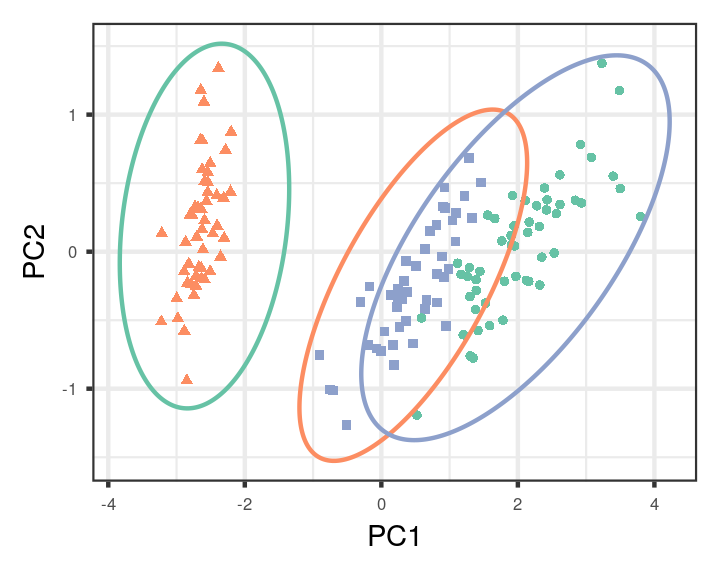
\includegraphics[width=0.588\linewidth,height=0.470\linewidth]{figure/iris_fit-1} 

}

\caption[The iris data in principal component space and 
                      GMM fit at $\alpha = 6$]{The iris data in principal component space and 
                      GMM fit at $\alpha = 6$. 
                      Colors denote inferred memberships and
                      ellipses are estimated covariances. }\label{fig:iris_fit}
\end{figure}


\end{knitrout}

We wish to evaluate the sensitivity of the expected number of clusters to the 
stick-breaking distribution. 
Define the expected number of \textit{in-sample} clusters as
\begin{align*}
\gclusters(\eta) &= \expect{\q(\z\vert\eta)}{\sum_{k=1}^\kmax \ind{ \sum_{n=1}^{N}
\z_{\n\k} > 0}} \\ 
&= \sum_{k=1}^\kmax \left(1 -  \prod_{n=1}^N
\left(1 - \expect{\q(\z_{nk}\vert\eta)}{\z_{nk}}\right)\right).
\end{align*}
The expectation and product can be interchanged because $q$ is mean-field. 

The in-sample quantity $\gclusters$ is an estimate for 
the number of species present in the observed iris dataset. 
Alternatively, we can define a {\itshape posterior predictive} quantity, 
which is an estimate of the number of species one would expect to see 
should a new iris dataset of size $N$ be collected.
Define the posterior predictive number of clusters as 
\begin{align}\eqlabel{post_pred_nclusters}
\gclusterspred(\eta) = \expect{\q(\nu\vert\eta)}{\sum_{k=1}^\kmax\left(1 -
(1 - \pi_k)^N\right)},
\end{align}
where recall that $\pi_k$ are the mixture weights computed from the stick-lengths, $\pi_\k = \nuk \prod_{\k' < \k} (1 - \nu_{\k'})$. 

Unlike the in-sample quantity, the expectation for the predictive quantity is not a simple closed-form function of the variational parameters.  
Instead, we approximate~\eqref{post_pred_nclusters} using Monte Carlo draws from the variational distribution. 
Specifically, we use the ``reparameterization trick" to sample from the variational distribution:
we use an appropriately chosen, $\eta$-dependent transformation 
$f(\cdot, \eta)$ that satisfies 
\begin{align*}
  u \iid\normdist{0, I} \implies 
  f(u, \eta) \stackrel{d}{=} \nu \sim \q(\cdot | \eta).
\end{align*}
To form a Monte Carlo estimate of \eqref{post_pred_nclusters}, 
we sample $u_1, ..., u_m\stackrel{iid}{\sim}\normdist{0, I}$ 
and then average the expression inside the expectation evaluated at points 
$f(u_1, \eta), ..., f(u_m, \eta)$.
We use the reparameterization trick so that conditional on $u_1, ..., u_m$,
our Monte Carlo estimate of $\gclusterspred$ is a determinstic function of 
the variational parameters $\eta$. 
In our experiments below, all displayed values of $\gclusterspred(\eta)$ are
Monte-Carlo approximations, 
conditional on the same $m = 10,000$ draws $u_1, ..., u_m$, fixed a priori. 

We evaluate the sensitivity of the posterior quantities 
$\gclusters$ and $\gclusterspred$ to the prior parameter $\alpha$ in the
$\betadist{\nuk \vert 1, \alpha}$ stick distribution. 
\figref{beta_priors} displays probability density functions of the stick distribution over a range of $\alpha$. 

We fit the initial model at $\alpha = 6$. 
Subsequent refits at $\alpha\not=6$ used the variational parameters at 
$\alpha = 6$ as an initialization. 
As $\alpha$ increases, both the expected in-sample and the expected predictive number of clusters increases (\figref{iris_alpha_sens}). 
The in-sample quantity is relatively insensitive to changes in the $\alpha$ parameter. 
As $\alpha$ varies from $\alpha = 1, ..., 16$, $\gclusters$ varies 
only from 3.0 to 3.4 (recall that the true number of iris species is three). 
On the other hand, the posterior preditive quantity is sensitive 
to changes in $\alpha$.
Over the same range of $\alpha$, $\gclusterspred$ varies from 
3.6 to 8.1. 

We computed the linear approximation at $\alpha = 6$.  
The linear approximation is able to reproduce changes to both 
the in-sample and predictive quantities found by refitting the model at each
$\alpha = 1, ..., 16$ (\figref{iris_alpha_sens}).  
Furthermore, the linear approximation is an order of magnitude faster than refitting. 
Forming the linear approximation, which requires a Hessian inversion (\eqref{vb_eta_sens}), required 0.02 seconds. 
After forming the linear approximation at $\alpha = 6$,
computing $\etalin(\alpha)$ for all $\alpha = 1, ... 16$ took another 
0.02 seconds.
On the other hand, to refit $\etaopt(\alpha)$ for the same range of
$\alpha$'s took a total of 10 seconds, 
with a median refit time of 0.7 seconds. 




\begin{knitrout}
\definecolor{shadecolor}{rgb}{0.969, 0.969, 0.969}\color{fgcolor}\begin{figure}[!h]

{\centering 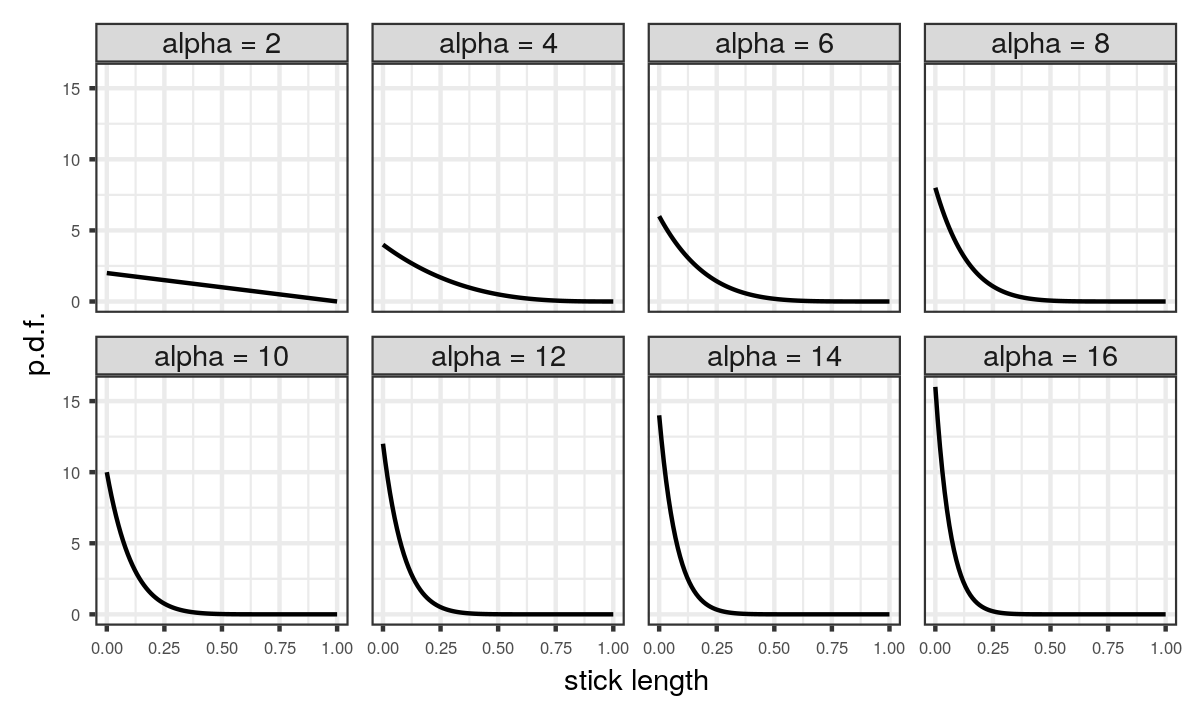
\includegraphics[width=0.980\linewidth,height=0.588\linewidth]{figure/beta_priors-1} 

}

\caption[Probability density functions of $\text{Beta}(1, \alpha)$ distributions, for various $\alpha$]{Probability density functions of $\text{Beta}(1, \alpha)$ distributions, for various $\alpha$. }\label{fig:beta_priors}
\end{figure}


\end{knitrout}




\begin{knitrout}
\definecolor{shadecolor}{rgb}{0.969, 0.969, 0.969}\color{fgcolor}\begin{figure}[!h]

{\centering 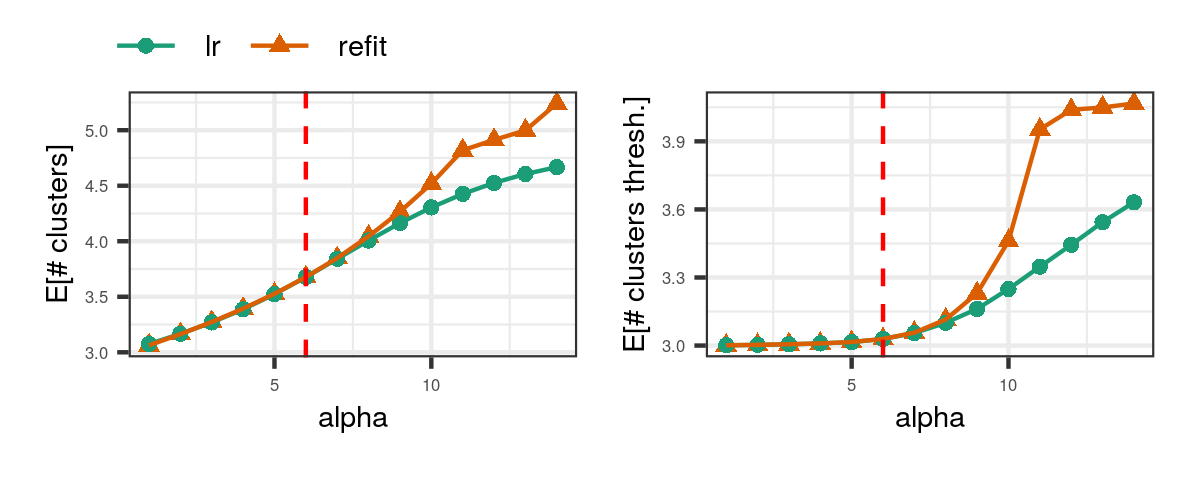
\includegraphics[width=0.980\linewidth,height=0.392\linewidth]{figure/iris_alpha_sens-1} 

}

\caption[The expected number of clusters as $\alpha$ varies in the 
the BNP-GMM fit of the iris data]{The expected number of clusters as $\alpha$ varies in the 
the BNP-GMM fit of the iris data. 
On the left is the sensitivity of the in-sample quantity.  
On the right is the the predictive quantity. 
We compute the linear approximation at $\alpha=6$ and
extrapolate the expected number of clusters using the
linear approximation (green).
We compare against the expected number of clusters obtained by refitting the model at each $\alpha$ (orange). }\label{fig:iris_alpha_sens}
\end{figure}


\end{knitrout}


% 
% - we demonstrate the utility of the influence function 
% - figure ref top three rows shows three different functional perturbations. 
% - can't really tell from densities how these will affect posterior statistic
% - but they do in fact have very different effects (in sign and size). 
% - but their effects make sense when looking at the influence function
% 
% -last row is worst-case

We next consider functional perturbations, 
and we demonstrate the ability of the influence function to 
provide guidance on the anticipated effect of perturbations 
on the posterior quantity. 
Each row of \figref{iris_fsens} presents a different 
multiplicative perturbation $\phi$ to the initial $\betadist{1, 6}$ stick distribution. 
The left column of \figref{iris_fsens} displays the perturbation $\phi$ overlayed with the prior-weighted influence function for $\gclusters$.
The perturbations are of the form 
$\log \phi(x) = e^{2(x - \mu)^2}$, with each perturbation having a 
different value of $\mu$. 
The middle column displays the initial density,
$p_0(\nu_k) = \betadist{\nu_k\vert 1, 6}$, along with the perturbed density,
$p_1(\nu_k) = \betadist{\nu_k\vert 1, 6}\phi(\nu_k)$.

Each perturbation $\phi$ produces distinct changes in the expected number of in-sample clusters $\gclusters$ (\figref{iris_fsens} right column). 
The changes in $\gclusters$ after each perturbation are 
different in both sign and magnitude. 
By examining the perturbed densities alone, it is difficult to anticipate 
the effect of the perturbation on $\gclusters$. 
However, the sign and magnitude of the change in $\gclusters$ is well-explained by the influence function. 
When $\log\phi$ is centered at a location where the influence function is negative, the effect on $\gclusters$ is negative (top row); 
conversely, when $\log\phi$ is centered at a location where the influence function is positive, the effect on $\gclusters$ is positive (bottom row); finally, when $\log\phi$ is centered at a location where the influence is both negative and positive, the effects cancel, and the change in the posterior statistic is roughly zero (middle row). 
In each case, the linear approximation is able to capture the changes in the posterior statistic. 
In applications below, we use influence function to guide our choice of functional perturbaton and to explain why some perturbations result in greater sensitivity than others. 

Finally, we consider the 
worst-case perturbation with unit $L_\infty$ norm.
Recall that the worst-case perturbation with unit $L_\infty$ norm is a 
step-function taking on values $\pm1$ corresponding 
to the sign of the influence function (\figref{iris_worstcase} left).  
The middle column of \figref{iris_worstcase} shows the prior density perturbed by the worst-case perturbation; 
the right column shows the effect on $\gclusters$. 
We see that this worst-case perturbation has a much larger effect on
$\gclusters$ compared to the other unit $L_\infty$ norm perturbations in
\figref{iris_fsens}. 
However, even with the worst-case perturbation, 
the change in $\gclusters$ is still small;
we thus conclude that in the iris dataset $\gclusters$ appears to be a quantity insensitive to the prior. 



\begin{knitrout}
\definecolor{shadecolor}{rgb}{0.969, 0.969, 0.969}\color{fgcolor}\begin{figure}[!h]

{\centering 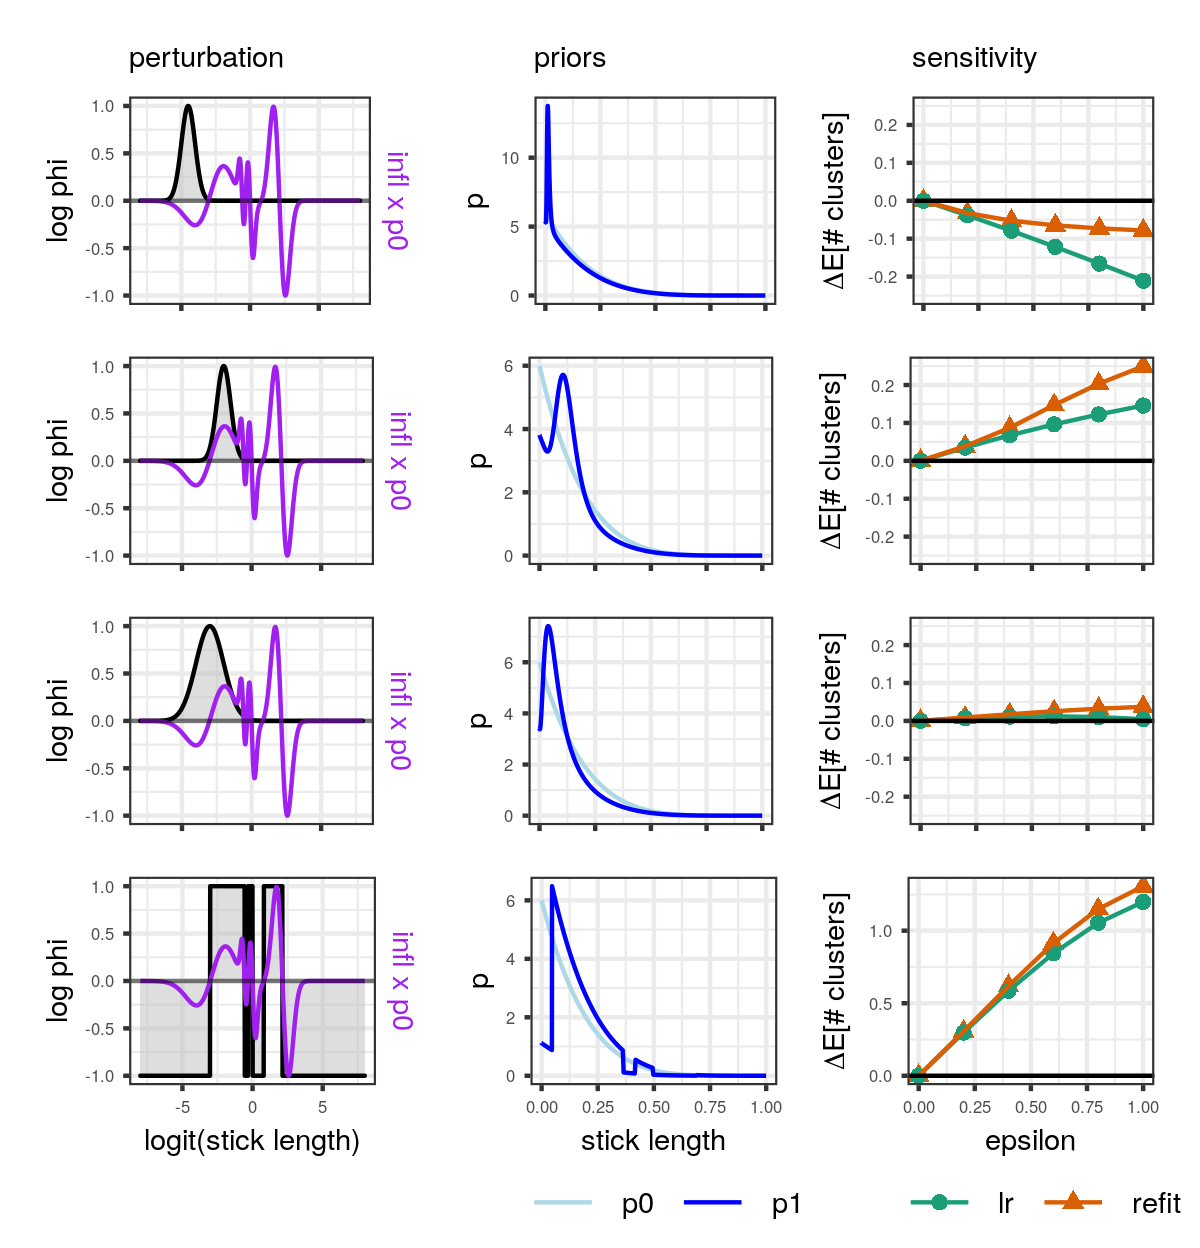
\includegraphics[width=0.980\linewidth,height=0.862\linewidth]{figure/iris_fsens-1} 

}

\caption{Sensitivity of
        the expected number of in-sample clusters in the iris dataset
        to three multiplicative perturbations with 
        unit $L_{\infty}$-norm 
        (Left) The log multiplicative perturbation $\log\phi$ in grey.        
        In purple is the prior-weighted influence function, scaled to also have 
        unit $L_{\infty}$-norm. 
        (Middle) The original prior density $p_0$ and 
        the perturbed prior density $p_1 = p_0\times \phi$. 
        (Right) The effect of the perturbation 
        on the change in expected number of clusters as a function of $\epsilon$. }\label{fig:iris_fsens}
\end{figure}


\end{knitrout}


\begin{knitrout}
\definecolor{shadecolor}{rgb}{0.969, 0.969, 0.969}\color{fgcolor}\begin{figure}[!h]

{\centering 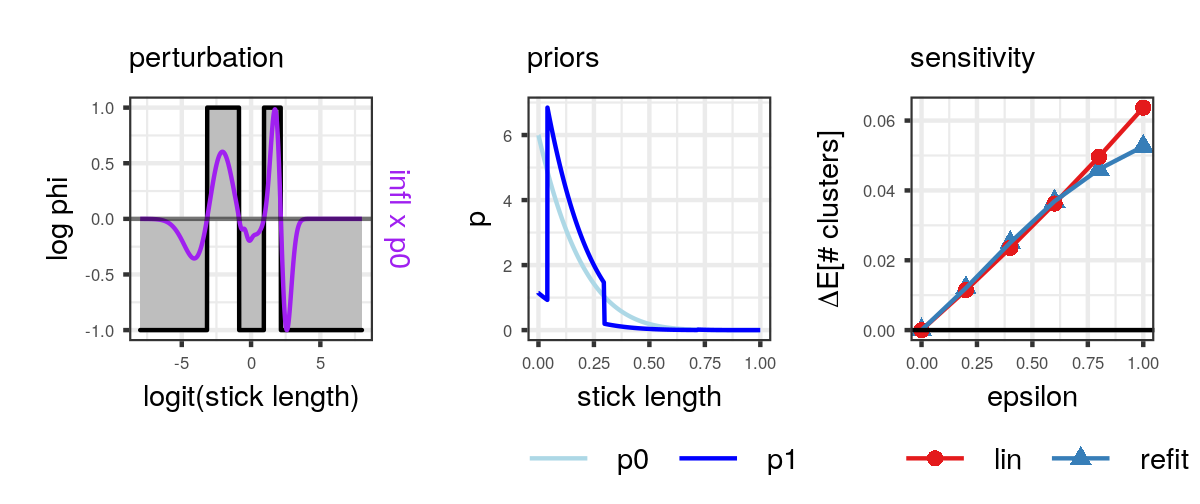
\includegraphics[width=0.980\linewidth,height=0.412\linewidth]{figure/iris_worstcase-1} 

}

\caption[Sensitivity of
        the expected number of in-sample clusters in the iris dataset
        to the worst-case multiplicative perturbations with 
        unit $L_{\infty}$-norm]{Sensitivity of
        the expected number of in-sample clusters in the iris dataset
        to the worst-case multiplicative perturbations with 
        unit $L_{\infty}$-norm.}\label{fig:iris_worstcase}
\end{figure}


\end{knitrout}

% \begin{table}[tb]
% \centering
% \caption{Compute time of results on the iris dataset. }
% \begin{tabular}{|r|r|}
%     \hline 
%     & time (seconds) \\ 
%     \hline 
%     Initial fit & sprintf('%1.2g', init_fit_time) \\
%     \hline 
%     Hessian solve for $\alpha$ sensitivity & 
%         sprintf('%1.2g', alpha_hess_time)\\
%     Linear approx. $\eta^{lin}(\alpha)$ for $\alpha = 1, ... , 16$ & 
%         sprintf('%1.2g', total_alpha_lr_time)\\
%     Refits $\eta(\alpha)$ for $\alpha = 1, ... , 16$ & 
%         sprintf('%1.2g', total_alpha_refit_time)\\
%     \hline 
%     The influence function & sprintf('%1.2g', infl_time)\\ 
%     Hessian solve for worst-case $\phi$ & 
%         sprintf('%1.2g', wc_hessian_time)\\
%     Linear approx. $\eta^{lin}(\epsilon)|_{\epsilon = 1}$
%     for worst-case $\phi$ & 
%         sprintf('%1.2g', wc_lr_time)\\
%     Refit $\eta(\epsilon)|_{\epsilon = 1}$ for worst-case $\phi$ & 
%         sprintf('%1.2g', wc_refit_time)\\ 
%     \hline 
% \end{tabular}
% \end{table}



    \subsection{Regression mixture modeling}
    \seclabel{results_mice}
    %%%%%%%%%%%%%%%%%%%%%%%%%%%%%%%%%%%%%%
%%%%%%%%%%%%%%%%%%%%%%%%%%%%%%%%%%%%%%
% Do not edit the TeX file your work
% will be overwritten.  Edit the RnW
% file instead.
%%%%%%%%%%%%%%%%%%%%%%%%%%%%%%%%%%%%%%
%%%%%%%%%%%%%%%%%%%%%%%%%%%%%%%%%%%%%%



We consider the problem of clustering time-course gene expression data. 
While thousands of genes might be simultaneously 
measured in a given genomics experiment, 
many genes may exhibit similar expression patterns.  
Clustering gene expressions
is one way to reduce the dimensionality of a complex data set 
and to facilitate scientific interpretations of intricate biological processes. 
Often, such dimensionality reduction is used for exploratory analysis and
is a first step before further downstream investigation.  
It is important, therefore, to acertain the stability of the 
discovered clusters. 
 
We study a publicly available data set of mice gene expression
\citep{shoemaker:2015:ultrasensitive}.
Mice were infected with different influenza viruses, and expression levels of a set of genes were assessed at 14 time points after infection.
Our analysis focuses on mice treated with the ``A/California/04/2009'' strain. 
We normalize the data as described in
\citet{shoemaker:2015:ultrasensitive} and then apply the differential
analysis tool EDGE \citep{Storey:2005:significance} to rank the genes from most to least significantly differentially expressed. 
We fit a BNP model and run our analysis below on the top $\ngenes = 1000$ genes.

\subsubsection*{The model}

Each gene consists of $\ntimepoints = 42$ measurements of expression: three measurements (called biological replicates) at 14 unique timepoints.
The timepoints are unevenly spaced, with more frequent observations at the beginning. 
Following \citet{Luan:2003:clustering} we apply cubic B-splines to smooth the time course expression data. 
Specifically, we model the first 11 timepoints using
cubic B-splines with 7 degrees of freedom.
For the last three timepoints, $\timeindx = 72, 120, 168$ hours,
we use indicator functions. 
That is, if $\tilde \regmatrix$ is the design 
matrix where each column is a
B-spline basis vector evaluated at the $\ntimepoints$ measurement times, 
we append to $\tilde \regmatrix$ three additional columns: 
in these columns, entries are 1
if $\timeindx = 72, 120,$ or 168, repectively, and 0 otherwise. 
Call the full design matrix $\regmatrix$. 
We use indicators for the last three timepoints for numerical stability; 
without the indicator columns,
the matrix $\tilde \regmatrix^T \tilde \regmatrix$ is nearly singular
because the later timepoints are more spread out. 
See \figref{example_genes} for an example gene and the B-spline basis. 

%

\begin{knitrout}
\definecolor{shadecolor}{rgb}{0.969, 0.969, 0.969}\color{fgcolor}\begin{figure}[!h]

{\centering 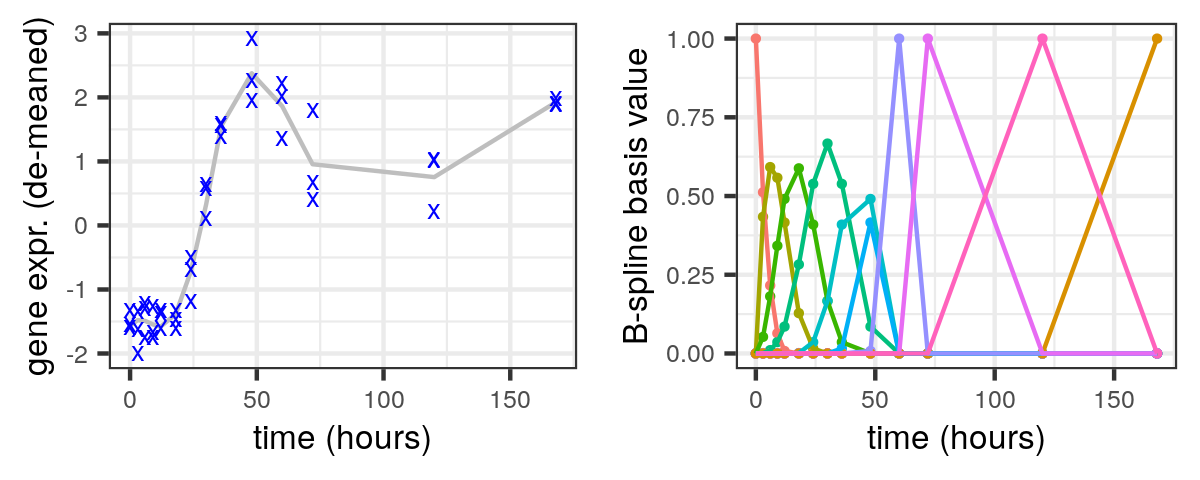
\includegraphics[width=0.980\linewidth,height=0.392\linewidth]{figure/example_genes-1} 

}

\caption[(Left) An example gene and its expression measured at 14 unique timepoints
    with three biological replicates at each timepoint.
     (Right) The cubic B-spline basis with 7 degrees of freedom, 
    along with three indicator functions for the last three timepoints, 
    $\timeindx = 72, 120, 168$]{(Left) An example gene and its expression measured at 14 unique timepoints
    with three biological replicates at each timepoint.
     (Right) The cubic B-spline basis with 7 degrees of freedom, 
    along with three indicator functions for the last three timepoints, 
    $\timeindx = 72, 120, 168$.}\label{fig:example_genes}
\end{figure}


\end{knitrout}
%


Let $\x_\n$ be the vector of observations for gene $\n$,
$(\x_{\n 1}, ..., \x_{\n \ntimepoints})^T$.
Each cluster is characterized by a vector of regression coefficients 
$\beta_k$ and a variance $\tau^{-1}_k$; 
the cluster parameters are $\theta_k = (\beta_k, \tau_k)$. 
The distribution of the data arising from cluster $k$ is 
\begin{align*}
\p(\x_\n | \theta_k, \b_{n}) = 
\normdist{\x_\n | \regmatrix\beta_k + \b_{n},
\tau_k^{-1}I_{\ntimepoints \times \ntimepoints}},
\end{align*}
where $\b_{n}$ is a gene-specific additive offset. 
We include the additive offset because we 
are interested in clustering the pattern of gene expression, 
not the absolute level. 

The joint distribution can be written in the same form as~\eqref{bnp_model}, 
except that the conditional log-likelihood also conditions on $b_n$, 
and we also include an additional prior term:
\begin{align*}
\MoveEqLeft
\logp(\x, \theta, \z, \nu) ={}
\nonumber\\&
    \sum_{n=1}^N \sum_{k=1}^{\kmax}
        \z_{\n\k} \left(
            \logp(\x_n \vert \theta_\k, \b_n) + \logp(\b_n) + \log \pi_\k
        \right) +
    \sum_{k=1}^{\kmax} \left(
        \log \pstick(\nuk) + \logp(\theta_\k)
    \right).
\end{align*}
We use a normal prior for the shifts $\b_n$, 
a multivariate normal prior for the coefficients $\beta_n$,
and a gamma prior for the inverse variance $\tau$. 

Our variational distribution factorizes as~\eqref{vb_mf}
with the addition
of a factor for the additive shift: 
\begin{align*}
\q(\zeta \vert \eta) =
    \left( \prod_{\k=1}^{\kmax - 1} \q(\nuk \vert \eta) \right)
    \left( \prod_{\k=1}^{\kmax} \q(\theta_\k \vert \eta) \right)
    \left( \prod_{\n=1}^{\N} \q(\z_{\n} \vert \eta) 
    \q(\b_{\n} \vert \z_{\n}, \eta)\right).
\end{align*}
Note that the variational distribution for $\b_\n$ conditions on $\z$.
We set $\q(\b_{\n} \vert \z_{\n} = k, \eta)$ to be Gaussian
with variational parameters dependent on $\k$. 
For simplicity in this application,
we let $\q(\theta_\k \vert \eta) = \delta (\theta_k \vert \eta)$, 
where $\delta(\cdot \vert \eta)$ denotes a point mass at a parameterized location. 

By parameterizing 
$\q(\z_{\n}, \b_{\n} \vert \eta) = \q(\z_{\n} \vert \eta)  \q(\b_{\n} \vert \z_{\n}, \eta)$ 
the optimal variational parameters for $\q(\z_{\n}, \b_{\n} \vert \eta)$ 
have a closed form given $\q(\nu, \theta \vert \eta)$. See \secref{put_in_appendix}. Therefore, our model fits the global/local framework as discussed in ... 
\todo{need to work on a section that talks about this}

We fitted the initial approximate posterior at $\alpha_0 = 6$. 
\figref{gene_centroids} shows the inferred smoothers 
$\regmatrix\mathbb{E}_\q[\beta_k]$ for selected clusters. 
\figref{gene_initial_coclustering} displays the inferred co-clustering matrix
$\coclusteringmatr(\eta)$, whose $(i,j)$-th entry is the
posterior probability that gene $i$ belongs to the same cluster
as gene $j$, given by 
\begin{align*}
\coclusteringmatr_{ij}(\eta) 
&= \expect{\q(\z\vert\eta)}{\ind{\z_{i} = \z_{j}}} \\
&= \sum_{k=1}^{\kmax}\left(\expect{\q(\z_i\vert\eta)}{\z_{ik}}
\expect{\q(\z_j\vert\eta)}{\z_{jk}}\right).
\end{align*}

Below, we evaluate the sensitivity of the inferred co-clustering matrix to 
both parametric and functional perturbations to the stick distribution. 


\begin{knitrout}
\definecolor{shadecolor}{rgb}{0.969, 0.969, 0.969}\color{fgcolor}\begin{figure}[!h]

{\centering 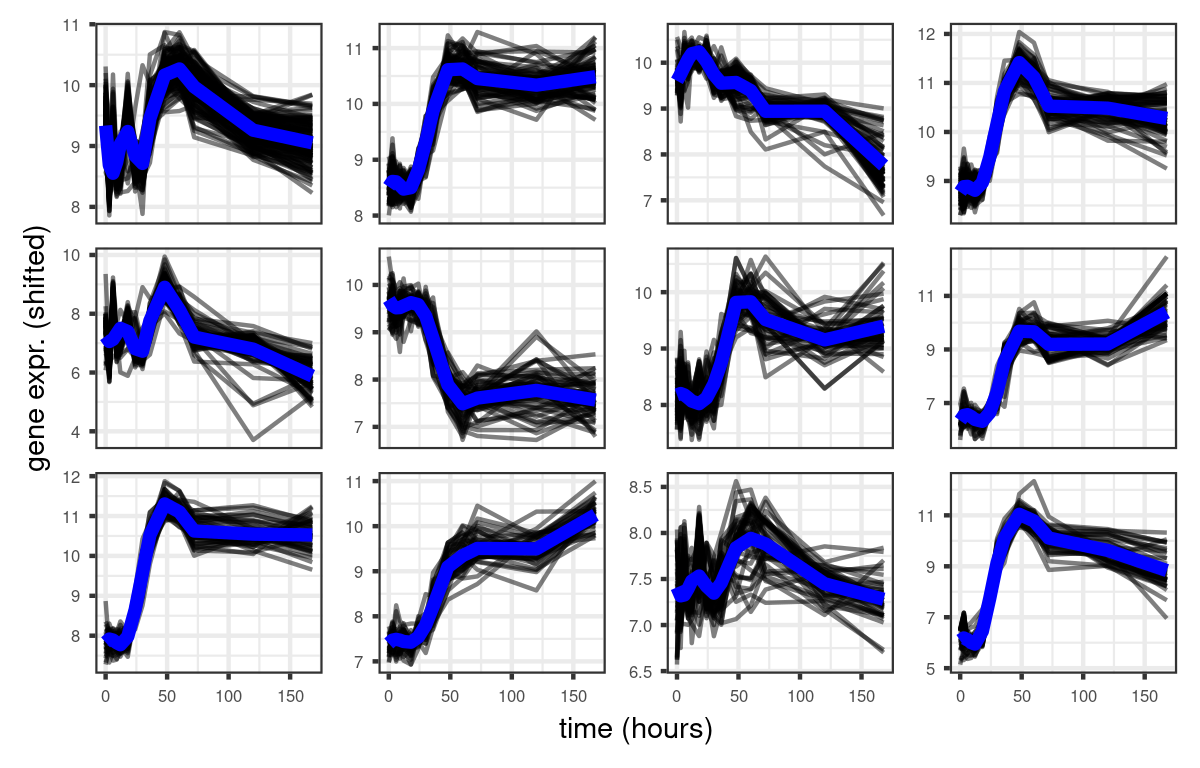
\includegraphics[width=0.980\linewidth,height=0.627\linewidth]{figure/gene_centroids-1} 

}

\caption[Inferred clusters in the mice gene expression dataset]{Inferred clusters in the mice gene expression dataset. 
    Shown are the twelve most occupied clusters. 
    In blue, the inferred cluster centroid. 
    In grey, gene expressions averaged over replicates and
    shifted by their inferred intercepts. }\label{fig:gene_centroids}
\end{figure}


\end{knitrout}



\begin{knitrout}
\definecolor{shadecolor}{rgb}{0.969, 0.969, 0.969}\color{fgcolor}\begin{figure}[!h]

{\centering 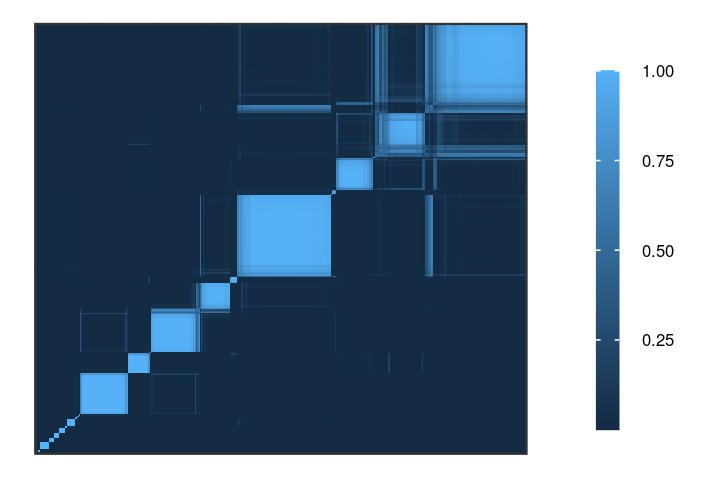
\includegraphics[width=0.588\linewidth,height=0.400\linewidth]{figure/gene_initial_coclustering-1} 

}

\caption[The inferred co-clustering matrix of gene expressions at $\alpha_0 = 6.$ ]{The inferred co-clustering matrix of gene expressions at $\alpha_0 = 6.$ }\label{fig:gene_initial_coclustering}
\end{figure}


\end{knitrout}


\subsubsection*{Sensitivity analysis}

We first evaluate the sensitivity of the co-clustering matrix $\coclusteringmatr$ 
to the choice of $\alpha$ in the
$\betadist{\nuk \vert 1, \alpha}$ stick distribution. 
Let $\coclusteringmatr_0 := \coclusteringmatr(\etaopt(\alpha_0))$ be the co-clustering matrix inferred at $\alpha_0$, 
and let $\Delta\coclusteringmatr(\eta) := 
\coclusteringmatr(\eta) - \coclusteringmatr_0$ be 
the difference in co-clustering matices after a change in the variational parameters $\eta$. 
We formed the linear approximation at $\alpha_0$ and computed
the change in co-clustering under the linearly approximated 
variational parameters, 
$\Delta\coclusteringmatr(\etalin(\alpha))$, at $\alpha = 1$ and $\alpha = 11$. 
For either $\alpha$, the change in the co-clustering matrix 
is miniscule (\figref{gene_alpha_coclustering}):
the largest entry of either matrix $\Delta\coclusteringmatr(\etalin(1))$ 
or $\Delta\coclusteringmatr(\etalin(11))$ is of order $10^{-2}$. 
Refitting the approximate posterior at $\alpha = 1$ and $\alpha = 11$ 
and computing $\Delta\coclusteringmatr(\etaopt(\alpha))$
confirms the insensitivity predicted by the linear approximation. 
Beyond capturing insensitivity, the linear approximation was also able to
approximate the sign and size of the changes in the individual entries of the coclustering matrix (these changes abeit small).  


\begin{knitrout}
\definecolor{shadecolor}{rgb}{0.969, 0.969, 0.969}\color{fgcolor}\begin{figure}[!h]

{\centering 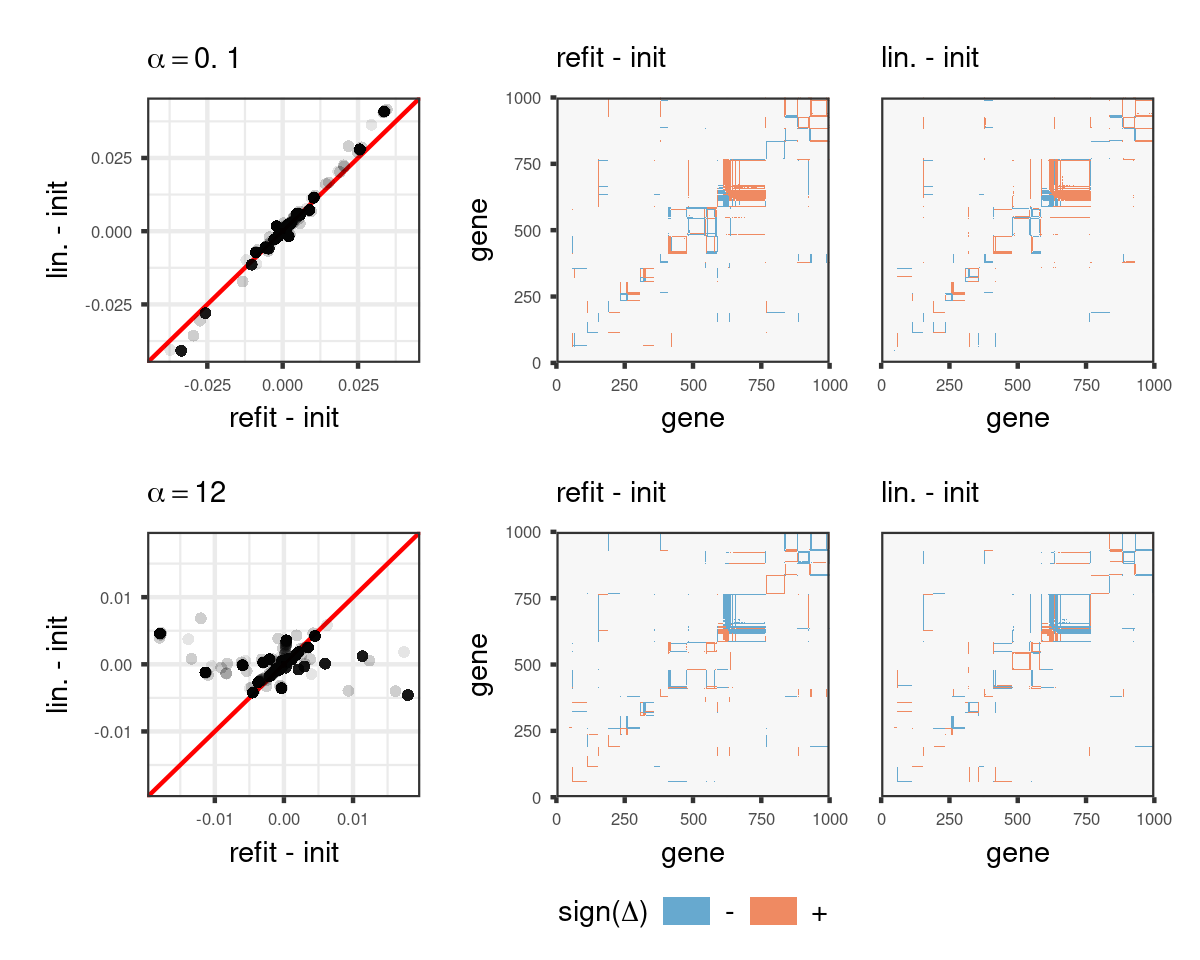
\includegraphics[width=0.980\linewidth,height=0.784\linewidth]{figure/gene_alpha_coclustering-1} 

}

\caption[Differences in the 
     co-clustering matrix at $\alpha = 1$ (top row)
     and $\alpha = 11$ (bottom row),
     relative to the co-clustering matrix at $\alpha_0 = 6$.
     We compare differences obtained with the linearly approximated 
     variational parameters against changes observed after 
     refiting]{Differences in the 
     co-clustering matrix at $\alpha = 1$ (top row)
     and $\alpha = 11$ (bottom row),
     relative to the co-clustering matrix at $\alpha_0 = 6$.
     We compare differences obtained with the linearly approximated 
     variational parameters against changes observed after 
     refiting. 
     (Left) a scatter plot of differences under the linear approximation 
     against differences after refitting, where
     each point represents an entry of the co-coclustering matrix.
     (Middle) the difference in co-clustering matrix observed after refitting. 
     (Right) the difference observed under the linearly approximated variational
     parameters. 
     For visualization, values in the heatmaps
     are clipped at $\pm 10^{-3}$. }\label{fig:gene_alpha_coclustering}
\end{figure}


\end{knitrout}


Insensitivity to $\alpha$ does not necessarily rule out insensitivity to other prior perturbations, however. 
As demonstrated in \secref{results_iris},
the influence function can provide guidance on which functional perturbations may result in greater sensitivity for a chosen posterior quantity. 
However, the co-clustering matrix as a posterior quantity is 
$\ngenes^2$-dimensional and 
thus does not lend itself to an easily interpretable influence function. 
We therefore summarize the co-clustering matrix into a scalar quantity: 
we use the sum of the eigenvalues of the symmetrically normalized graph Laplacian. 
This quantity has close connection with 
the number of distinct components in a graph CITE. 
Let this posterior quantity be denoted $\laplacianevsum$, given by 
\begin{align*}
  \laplacianevsum(\eta) = 
  \text{Tr}\left(
  I - D(\eta)^{-1/2} \coclusteringmatr(\eta) D(\eta)^{-1/2}
  \right),
\end{align*}
where $D(\eta)^{-1/2}$ is the diagonal matrix with entries $d_i = \sum_{j=1}^{\ngenes}[\coclusteringmatr(\eta)]_{ij}$. 
(And recall that the trace of a matrix is equivalent to the sum of its eigenvalues).

Because $\laplacianevsum(\eta)$ is a scalar quantity, we can plot its influence function. 
We choose a functional perturbation $\log\phi_{\textrm{ev}}$ that has a large, positive inner-product with the influence function.
In this case, we construct $\log\phi_{\textrm{ev}}$
using two Gaussian bumps aligned with
the two largest modes of the prior-weighted influence function
(\figref{gene_fpert_coclustering} top left). 
We anticipate $\log\phi_{\textrm{ev}}$
to have a large effect on $\laplacianevsum$. 
With $\laplacianevsum$ a proxy for our actual posterior quantity of interest, 
the full co-clustering matrix, we then expect that the co-clustering matrix 
will also experience large changes. 





Our intuition is confirmed in \figref{gene_fpert_coclustering}. 
After perturbing by $\log\phi_{\textrm{ev}}$, 
the largest changes in the co-clustering matrix are of now of order $10^{-1}$, 
compared with changes on the order of $10^{-2}$ after the $\alpha$ perturbations. 
The linear approximation again able to capture the qualitative changes in the co-clustering matrix after refitting at the perturbed prior. 


\begin{knitrout}
\definecolor{shadecolor}{rgb}{0.969, 0.969, 0.969}\color{fgcolor}\begin{figure}[!h]

{\centering 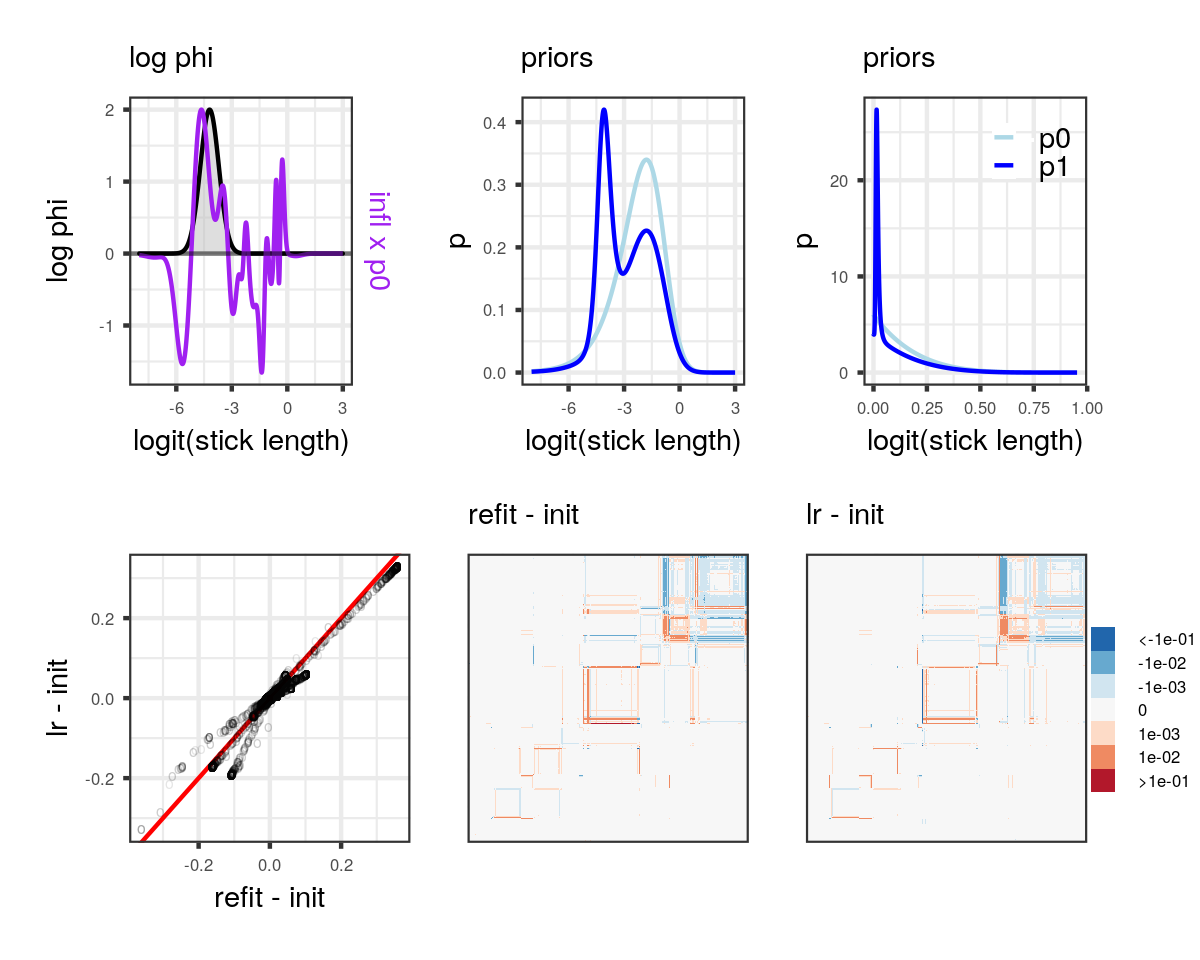
\includegraphics[width=0.980\linewidth,height=0.784\linewidth]{figure/gene_fpert_coclustering-1} 

}

\caption[Effect on the co-clustering matrix after a multiplicative functional
     perturbation.
     The perturbation $\phi$ (top left, in grey) 
     is a difference of two Gaussian bumps 
     scaled to have $L_\infty$ norm equal to two.
     $\phi$ is chosen such that the Gaussian bumps roughly align with the 
     two largest modes of the influence function (top left, purple]{Effect on the co-clustering matrix after a multiplicative functional
     perturbation.
     The perturbation $\phi$ (top left, in grey) 
     is a difference of two Gaussian bumps 
     scaled to have $L_\infty$ norm equal to two.
     $\phi$ is chosen such that the Gaussian bumps roughly align with the 
     two largest modes of the influence function (top left, purple; 
     the influence function is scaled to also have $L_\infty$ norm equal to two).
     The effect of this perturbation on the prior density in the top right. 
     The bottom row shows the effect of this perturbation on 
    the coclustering matrix.
    For visualization, the differences in the heatmap 
     are clipped at $\pm 10^{-1}$.}\label{fig:gene_fpert_coclustering}
\end{figure}


\end{knitrout}

The influence function is able to explain why the co-clustering matrix is 
insensitive to $\alpha$.
The functional perturbation
that corresponds to a change in $\alpha$ is
\begin{align*}
\log \phi_\alpha(\nu_\k) :=
\log\betadist{\nu_\k\vert 1, \alpha} -
\log\betadist{\nu_\k\vert 1, \alpha_0}.
\end{align*}
The function $\log\phi_\alpha(\nu_\k)$ is large when the influence function is small and vice-versa (\figref{alpha_pert_logphi}),
resulting in a small inner-product between the influence function
and $\log\phi_\alpha$. 
Thus, the linear approximation will predict small changes, and 
the refitted results confirms the linear approximation predictions. 


\begin{knitrout}
\definecolor{shadecolor}{rgb}{0.969, 0.969, 0.969}\color{fgcolor}\begin{figure}[!h]

{\centering 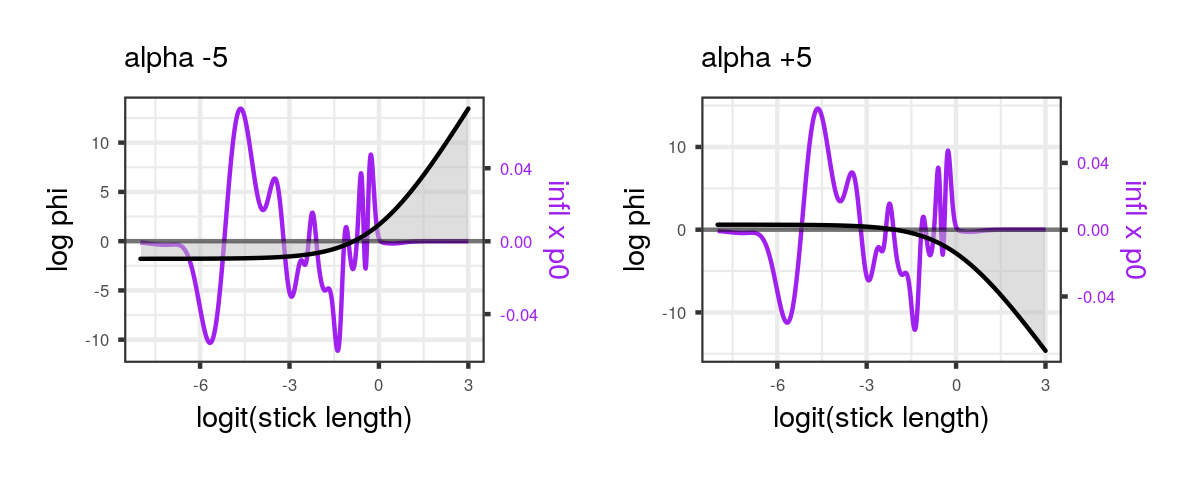
\includegraphics[width=0.882\linewidth,height=0.423\linewidth]{figure/alpha_pert_logphi-1} 

}

\caption[The multiplicative perturbations $\phi_\alpha(\cdot)$ that 
    corresponds to decreasing (left) or increasing (right) 
    the $\alpha$ parameter by five]{The multiplicative perturbations $\phi_\alpha(\cdot)$ that 
    corresponds to decreasing (left) or increasing (right) 
    the $\alpha$ parameter by five. }\label{fig:alpha_pert_logphi}
\end{figure}


\end{knitrout}

However, even with the selected functional perturbation,
the size of the differences in the co-clustering matrix remains modest. 
It is unlikely that any conclusions derived from the co-clustering matrix would have changed after the functional perturbation. 
The co-clustering matrix appears insensitive to perturbations in the stick-breaking distribution. 

Finally, we note that the computational cost of the linear approximation is again favorable compared with refitting (\tabref{mice_timing}). 
Forming the linear approximation, which requires a Hessian inversion, 
took 3-4 seconds; subsequent evaluations of $\etalin$ take milliseconds. 
Conversely, refitting the model after a prior perturbation can take up to 20 seconds. 

\begin{table}[tb]
\centering
\caption{Compute time of results on the mice data set. }
\tablabel{mice_timing}
\begin{tabular}{|r|r|}
    \hline 
    & time (seconds) \\ 
    \hline 
    Initial fit & 30 \\
    \hline 
    Hessian solve for $\alpha$ sensitivity & 
        3.9\\
    Linear approx. $\eta^{lin}(\alpha)$ for $\alpha = 1$ & 
        0.0013\\
    Linear approx. $\eta^{lin}(\alpha)$ for $\alpha = 11$ & 
        0.0012\\
    Refit $\eta(\alpha)$ for $\alpha = 1$ & 
        14\\
    Refit $\eta(\alpha)$ for $\alpha = 11$ & 
        13\\
    \hline
    The influence function & 4.3\\ 
    Hessian solve for $\phi$ perturbation &
        3.3\\
    Linear approx. $\eta^{lin}(\epsilon)$ at $\epsilon = 1$ &
        0.00099\\
    Refit $\eta(\epsilon)$ at $\epsilon = 1$ &
        22\\
    \hline
\end{tabular}
\end{table}


    \subsection{Genetic admixture modeling with fastSTRUCTURE}
    \seclabel{results_structure}
    %%%%%%%%%%%%%%%%%%%%%%%%%%%%%%%%%%%%%%
%%%%%%%%%%%%%%%%%%%%%%%%%%%%%%%%%%%%%%
% Do not edit the TeX file your work
% will be overwritten.  Edit the RnW
% file instead.
%%%%%%%%%%%%%%%%%%%%%%%%%%%%%%%%%%%%%%
%%%%%%%%%%%%%%%%%%%%%%%%%%%%%%%%%%%%%%



Our final data analysis example is an application of a Bayesian topic model to
population genetics. We consider a publicly available dataset from
\citet{galbusera:2000:thrush} that contains genotypes from 155 samples of an
endangered bird species, the Taita thrush. Individuals were collected from four
regions in southeast Kenya (Chawia, Mbololo, Ngangao, Yale), and each individual
was genotyped at seven micro-satellite loci. The four regions were once part of
a cohesive cloud forest that has since been fragmented by human development. For
this endangered bird species, understanding the degree to which populations have
grown genetically distinct is important for conservation efforts: well-separated
populations with little genetic diversity are particularly at risk of
extinction.  The goal of the analysis is to identify the presence of latent
populations, from which one can infer the population of origin for specific
loci, and estimate the degree to which populations are admixed in each
individual.


\subsubsection*{The model}

The data consists of consists of $\nindiv$ individuals genotyped at $\nloci$
loci. Let $\x_{\n\l\i}\in\{1, \ldots, J_\l\}$ be the observed genotype for
individual $\n$ at locus $\l$ and chromosome $\i$. $J_\l$ is the number of
possible genotypes at locus $\l$. For example, if the measurements are all
single nucleotides (A, T, C or G) then $J_\l = 4$ for all $\l$.

A latent population is characterized by the collection $\beta_k =
(\latentpop_{\k1}, \ldots, \latentpop_{\k\nloci})$ where
$\latentpop_{\k\l}\in\Delta^{J_\l - 1}$ are the latent frequencies for the $J_l$
possible genotypes at locus $\l$. Let $\z_{\n\l\i}$ be the assignment of
observation $\x_{\n\l\i}$ to a latent population. Notice that for a given
individual $\n$, different loci, or even different chromosomes at a given locus,
may have different population assignments. The distribution of
$\x_{\n\l\i}\in\{1, \ldots, J_\l\}$ arising from population $\k$ is
%
\begin{align*}
\p(\x_{\n\l\i} \vert \latentpop_{\k}) =
\categoricaldist{\x_{\n\l\i}\vert \latentpop_{\k\l}}.
\end{align*}

Unlike the previous models, we now have a stick-breaking process for each
individual. Draw sticks
%
\begin{align*}
\nu_{\n\k} \iid \pstick(\nu_{\n\k}) \quad \forall \n = 1, \ldots, \nindiv; \k = 1, 2, \ldots \infty.
\end{align*}
%
The prior assignment probability vector $\latentadmix_{\n} =
(\latentadmix_{\n1}, \latentadmix_{\n2}, \ldots)$, now unique to each
individual, is formed by the same stick-breaking construction as before,
%
\begin{align*}
\latentadmix_{\n\k} = \nu_{\n\k} \prod_{\k' < \k} (1 - \nu_{\n\k'}).
\end{align*}
%
The population assignment $\z_{\n\l\i}$ is drawn from the usual multinomial
distribution
%
\begin{align*}
p(\z_{\n\l\i} | \latentadmix_\n) = \prod_{k=1}^{\infty} \latentadmix_{\n\k}^{\z_{\n\l\i\k}}.
\end{align*}
%
In this genetics application, we call $\latentadmix_{\n}$ the \textit{admixture}
of individual $\n$.

This model is identical to fastSTRUCTURE, a model proposed in
\citet{pritchard:2000:structure, raj:2014:faststructure}, except that we replace
the Dirichlet prior in fastSTRUCTURE with an infinite stick-breaking process.
The result is a model similar to a hierarchical Dirichlet process for topic
modeling \citep{teh:2006:hdp}, but without the top-level Dirichlet process. In
addition, genotypes at genetic markers take the place of words in a document; in
lieu of inferring ``topics," we infer latent populations.

The variational approximation is mean-field as before, and all distributions are
conditionally conjugate except for the stick-breaking proportions, which remain
logit-normal. See \appref{app_structure} for further details.



\begin{knitrout}
\definecolor{shadecolor}{rgb}{0.969, 0.969, 0.969}\color{fgcolor}\begin{figure}[!h]

{\centering 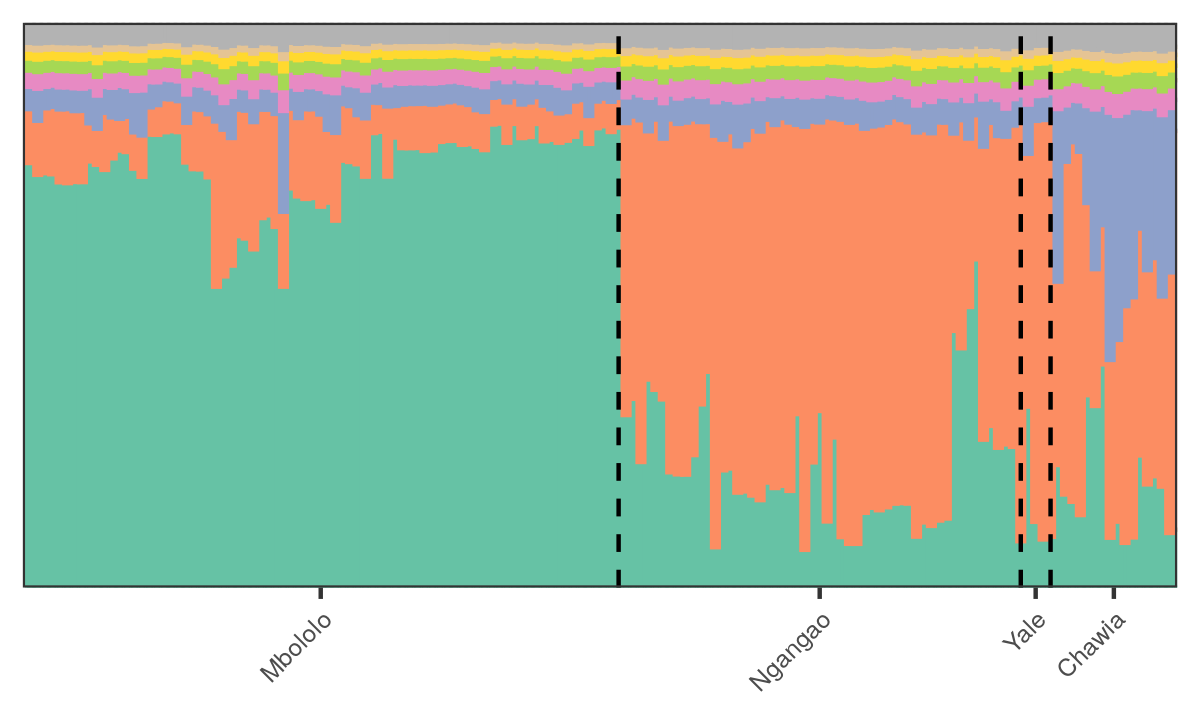
\includegraphics[width=0.980\linewidth,height=0.588\linewidth]{figure/stru_init_fit-1} 

}

\caption[The inferred individual admixtures at $\alpha_0 = 3$.
    Each vertical strip is an individual and each color
    a latent population.
    Lengths of colored segments represent the inferred admixture proportions.
    Individuals are ordered by the geographic region from which they were sampled
    (Mbololo, Ngangao, Yale, and Chawia).
    In the text, we refer to the green, orange, and purple latent populations
    as population 1, 2, and 3, respectively]{The inferred individual admixtures at $\alpha_0 = 3$.
    Each vertical strip is an individual and each color
    a latent population.
    Lengths of colored segments represent the inferred admixture proportions.
    Individuals are ordered by the geographic region from which they were sampled
    (Mbololo, Ngangao, Yale, and Chawia).
    In the text, we refer to the green, orange, and purple latent populations
    as population 1, 2, and 3, respectively. }\label{fig:stru_init_fit}
\end{figure}


\end{knitrout}

\subsubsection*{Quantity of interest}

The posterior quantities of interest in this application
are the individual admixtures $\pi_\n$.
\figref{stru_init_fit} plots the inferred admixtures $\pi_\n$ for all
individuals $\n$ under a $\gem$ prior with parameter $\alpha_0 = 3$.
The choice of $\alpha_0 = 3$ corresponds to roughly four distinct populations {\em a priori}, motivated by the fact that the individuals come from four geographic regions.
We will examine the robustness of the inferred admixtures to the prior below.

In the posterior at $\alpha_0$, there
appear to be three dominant latent populations, which we arbitrarily label as
populations 1, 2, and 3 (\figref{stru_init_fit}).
The inferred admixture proportions generally correspond with the geographic regions from which each individuals are sampled.

Notably, outlying admixtures among individuals from the same geographic region provide clues into the historical migration patterns of this species.
For example,
while individuals collected from the Mbololo region are inferred to be admixed
primarily with population 1, several individuals from this region have
abnormally large admixture proportions of population 2. Conversely, while
individuals collected from the Ngangao region are admixed primarily with
population 2, a few of these individuals have abnormally large admixture
proportions of population 1. This suggests that some migration has occurred
between the Mbololo and Ngangao regions.

We evaluate the sensitivity of this conclusion to possible prior perturbations.
Consider the posterior statistic
%
\begin{align*}
\gadmix(\eta; \mathcal{N}, k) =
 \expect{\q(\pi\vert\eta)}{\frac{1}{|\mathcal{N}|}\sum_{n\in\mathcal{N}}
\pi_{\n\k}},
\end{align*}
%
the average admixture proportion of population $\k$ in a set of
individuals $\mathcal{N}$.

Below, we present results on three variations of $\gadmix$, corresponding to
indididuals hightlighted as ``A," ``B", or ``C" in the top row of \figref{stru_func_sens}:
$\mathcal{N} = \{26, ..., 31\}$ and $k = 2$,
corresponding to the six individuals from the Mbololo region with outlying proportions of population 2;
$\mathcal{N} = \{125, ..., 128\}$ and $k = 1$,
corresponding to the four individuals from the Ngangao region with outlying proportions of population 1;
$\mathcal{N} = \{139, ..., 155\}$ and $k = 3$,
corresponding to all individuals from the Chawia region.
The first two posterior quantities relate to the inferred migration between
the Mbololo and Ngangao regions.
In the last case, we are studying the robustness of having a third latent
population present, a population which primarily appears in Chawia individuals.

\subsubsection*{Functional sensitivity}

In \figref{stru_func_sens}, we construct the worst-case negative perturbation
for decreasing each of our three variant of $\gadmix$, in order to see
whether the biologically interesting patterns can be made to disappear
with different prior choices.

\todo{Make the text easier to match up with the picture, which doesn't
have the populations (Ngangao, etc) labeled.  Right now it's hard to see
what's going on.}

\todo{I think this whole section could be easier to understand and much more
compact.  Basically just say that A is non-robust, B is robust, and on C
the linear approximation and refit disagree.  Then we investigate A more.}

Under the
linearized variational parameters $\etalinglobal(\t)$, the admixture proportion
of population 2 in the outlying Mbololo individuals is nearly halved.
The same quantity computed after refitting the model confirms the
sensitivity predicted by the linearized variational parameters.

 On the other
hand, the presence of population 1 in the outlying Ngangao individuals appears
to be insensitive even after this worst-case perturbation. The linearized and
the refitted variational parameters again agree on this conclusion. Finally, the
presence of population 3 in the Chawia individuals is anticipated to be
sensitive by the linearized parameters, as this admixture proportion steadily
decreases as $t\rightarrow 1$. However, under the refits, this admixture
proportion does not decrease steadily but rather levels off after $t = 0.5$.



\begin{knitrout}
\definecolor{shadecolor}{rgb}{0.969, 0.969, 0.969}\color{fgcolor}\begin{figure}[!h]

{\centering 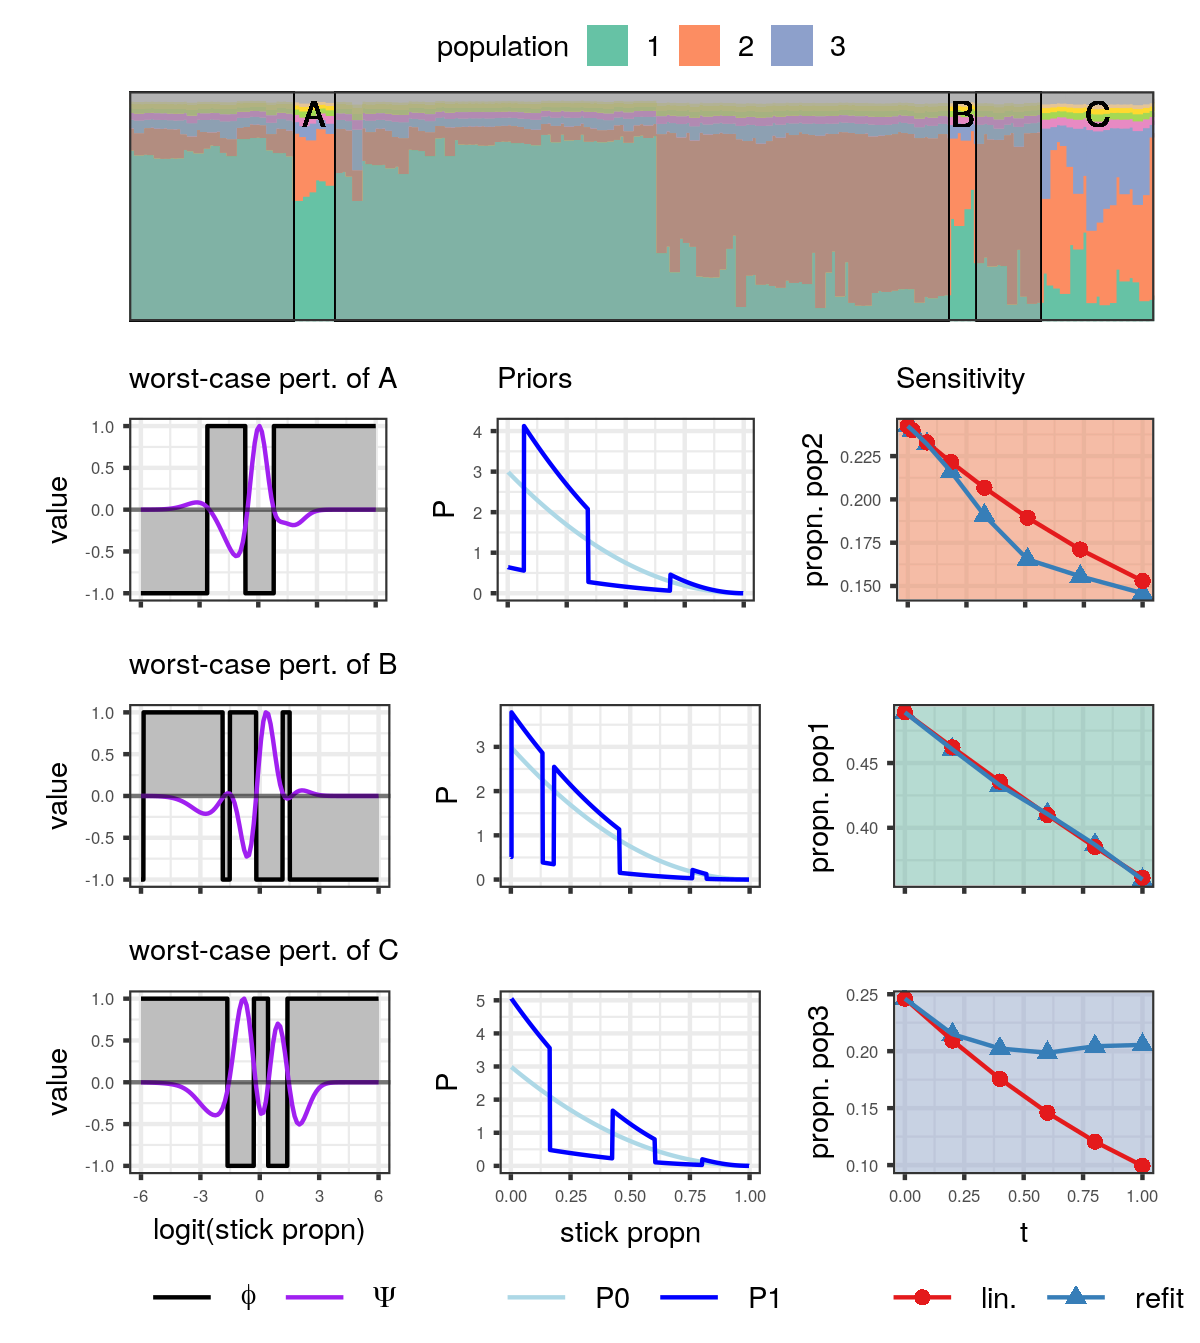
\includegraphics[width=0.980\linewidth,height=1.098\linewidth]{figure/stru_func_sens-1} 

}

\caption[Sensitivity of inferred admixtures for several outlying individuals.
     For individuals A,
     we examine the sensitivity of the admixture proportion of population 2.
     For individuals B,
     we examine the population 1 admixture
     For the individuals C, we examine the population 3 admixture.
     (Left column) The worst-case negative perturbation with
     $\norminf{\phi} = 1$
     in grey,
     plotted against the influence function in purple
     (scaled such that $\norminf{\psi} = 1$).
    (Middle column) The effect of the perturbation on the prior density.
    (Right column) Effects on the inferred admixture]{Sensitivity of inferred admixtures for several outlying individuals.
     For individuals A,
     we examine the sensitivity of the admixture proportion of population 2.
     For individuals B,
     we examine the population 1 admixture
     For the individuals C, we examine the population 3 admixture.
     (Left column) The worst-case negative perturbation with
     $\norminf{\phi} = 1$
     in grey,
     plotted against the influence function in purple
     (scaled such that $\norminf{\psi} = 1$).
    (Middle column) The effect of the perturbation on the prior density.
    (Right column) Effects on the inferred admixture. }\label{fig:stru_func_sens}
\end{figure}


\end{knitrout}


\todo{Say something about the fact that these priors are maybe too
adversarial.}


The conclusions from the linear approximation did not
perfectly agree with the conclusions from refitting variational approximation
in this data set and model.
For example, the admixture proportion of population 3 in individuals ``C" were predicted to be non-robust by our linear approximation but are in actuality are robust after refitting (bottom row \figref{stru_func_sens}).

Moreover, even though the linearized parameters
agreed with the refits in producing the diminished
overall admixture proportion of population 2 in individuals ``A"
(\figref{stru_func_sens} second row),
the approximation does does not perform uniformly well over all individual admixtures.
\figref{stru_func_sens_admix} plots the individual admixtures after the worst-case prior perturbation computed under both our linear approximation and after refitting.
The admixture proportion of population 2 in individual $n = 25$
dramatically increased after refitting with the perturbed prior $\p_1$;
the linearized parameters failed to reproduce this change.
For a more in depth discussion of the limitations of the linear approximation,
see \appref{app_structure_results}.

\todo{need to highlight main takeaway: even though linear approx works less well, still can use influence function to guide where to refit. }


\begin{knitrout}
\definecolor{shadecolor}{rgb}{0.969, 0.969, 0.969}\color{fgcolor}\begin{figure}[!h]

{\centering 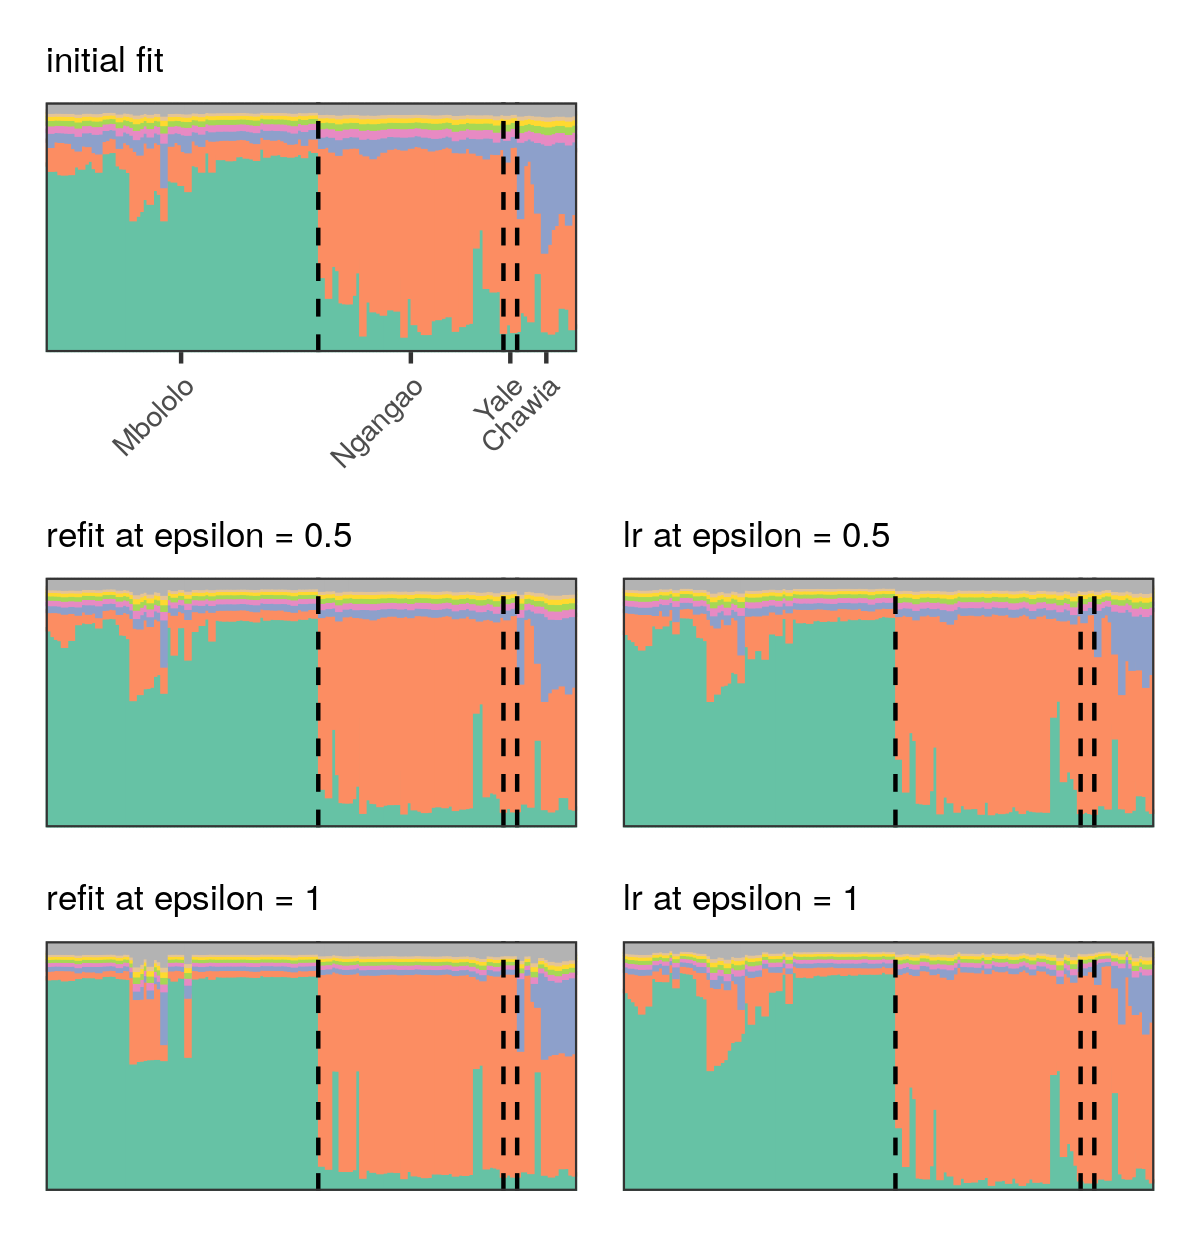
\includegraphics[width=0.980\linewidth,height=0.392\linewidth]{figure/stru_func_sens_admix-1} 

}

\caption{Inferred admixtures after the worst-case perturbation
     to individuals ``A" (see Figure~\ref{fig:stru_func_sens} for perturbation). }\label{fig:stru_func_sens_admix}
\end{figure}


\end{knitrout}


\newcommand{\StructureLimitationsA}{

\begin{knitrout}
\definecolor{shadecolor}{rgb}{0.969, 0.969, 0.969}\color{fgcolor}\begin{figure}[!h]

{\centering 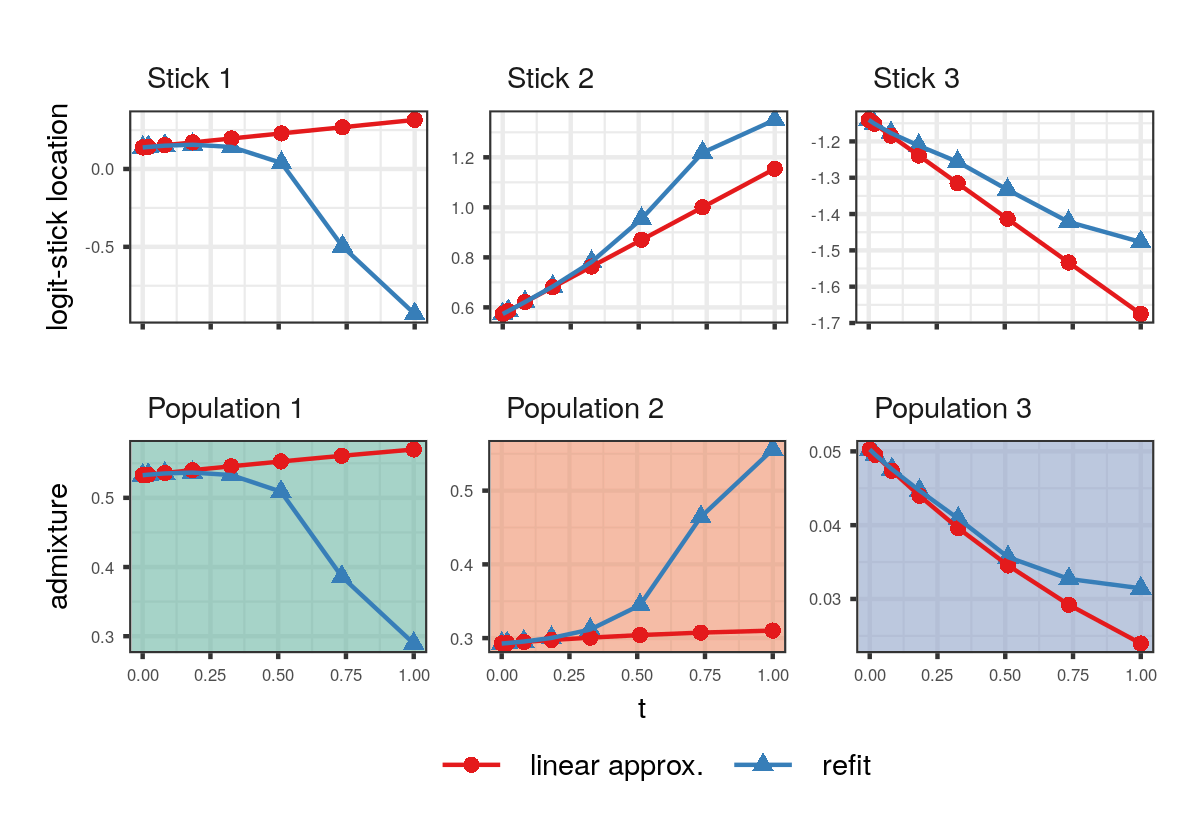
\includegraphics[width=0.980\linewidth,height=0.666\linewidth]{figure/stru_lin_bad_example-1} 

}

\caption[An individual $(\n = 26)$ for which
    the linearly approximated variational parameters
    poorly captured the
    change in admixture observed after refitting
    as $\t \rightarrow 1$.
    (Top row) the change in location parameter of the normally
    distributed logit-sticks, for the first three sticks.
    The response here is a variational parameter, so
    the approximation (red) is necessarily linear with respect to $\t$.
    (Bottom row) the change in the inferred admixtures for
    populations 1, 2, and 3]{An individual $(\n = 26)$ for which
    the linearly approximated variational parameters
    poorly captured the
    change in admixture observed after refitting
    as $\t \rightarrow 1$.
    (Top row) the change in location parameter of the normally
    distributed logit-sticks, for the first three sticks.
    The response here is a variational parameter, so
    the approximation (red) is necessarily linear with respect to $\t$.
    (Bottom row) the change in the inferred admixtures for
    populations 1, 2, and 3. }\label{fig:stru_lin_bad_example}
\end{figure}


\end{knitrout}
}

\newcommand{\StructureLimitationsB}{

\begin{knitrout}
\definecolor{shadecolor}{rgb}{0.969, 0.969, 0.969}\color{fgcolor}\begin{figure}[!h]

{\centering 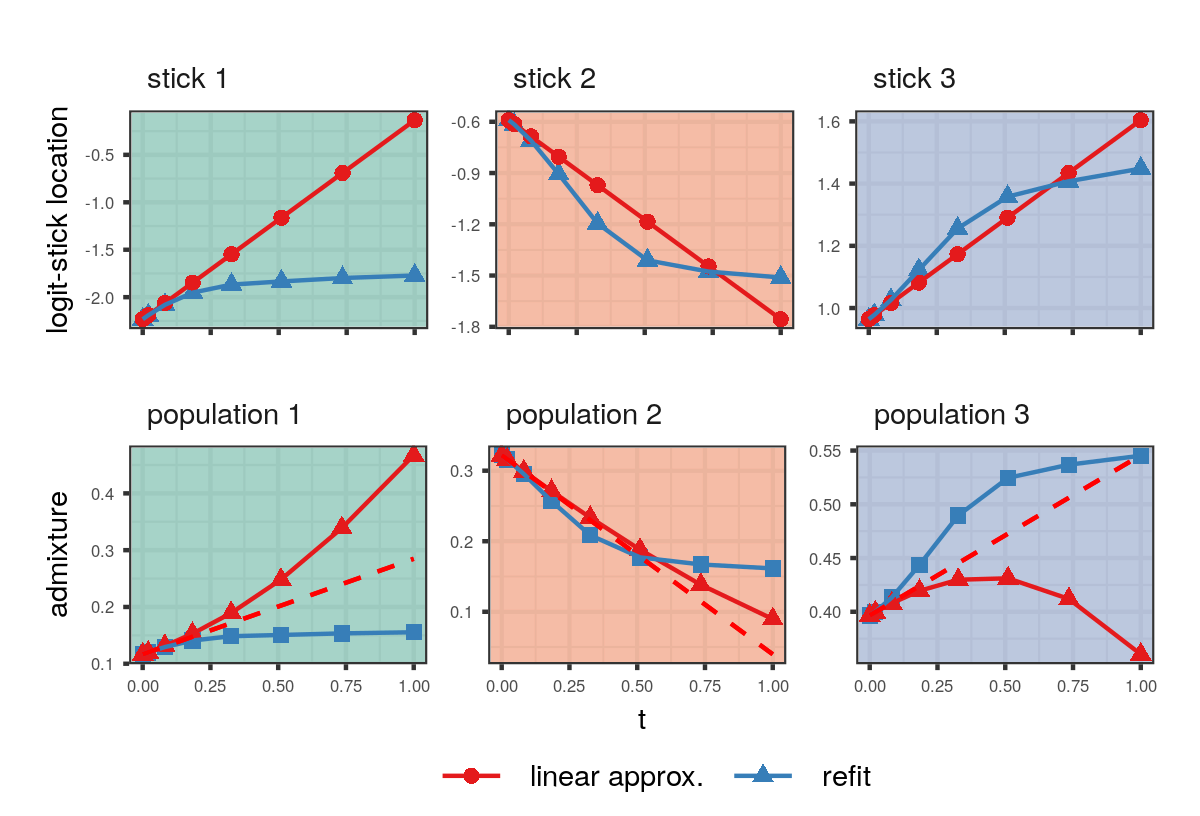
\includegraphics[width=0.980\linewidth,height=0.666\linewidth]{figure/stru_fully_lin_example-1} 

}

\caption[An example where
    linearizing the posterior quantity itself outperforms
    linearizing the variational parameters only.
    Shown are logit-stick location parameters (top row) and
    inferred admixtures (bottom row)
    for individual $n = 74$ and populations $k = 1, 2$ and $3$.
    Dashed red is the approximation $\glin(\t)$ formed by linearizing the
    inferred admixture $\expect{\q}{\pi_{\n\k}}$ with respect to prior
    parameter $t$.
    On the admixture proportion of population 3,
    $\glin(\t)$ outperforms $\g(\etalin(\t))$ (solid red)]{An example where
    linearizing the posterior quantity itself outperforms
    linearizing the variational parameters only.
    Shown are logit-stick location parameters (top row) and
    inferred admixtures (bottom row)
    for individual $n = 74$ and populations $k = 1, 2$ and $3$.
    Dashed red is the approximation $\glin(\t)$ formed by linearizing the
    inferred admixture $\expect{\q}{\pi_{\n\k}}$ with respect to prior
    parameter $t$.
    On the admixture proportion of population 3,
    $\glin(\t)$ outperforms $\g(\etalin(\t))$ (solid red). }\label{fig:stru_fully_lin_example}
\end{figure}


\end{knitrout}
}


    \subsection{Computation time}
    \seclabel{compute_time}
    %%%%%%%%%%%%%%%%%%%%%%%%%%%%%%%%%%%%%%
%%%%%%%%%%%%%%%%%%%%%%%%%%%%%%%%%%%%%%
% Do not edit the TeX file your work
% will be overwritten.  Edit the RnW
% file instead.
%%%%%%%%%%%%%%%%%%%%%%%%%%%%%%%%%%%%%%
%%%%%%%%%%%%%%%%%%%%%%%%%%%%%%%%%%%%%%



The relative computational costs of the approximation and re-fitting for our
three experiments are shown in \tabref{timing_table}. The data sets we
considered in our experiments had varying degrees of complexity, and the
computational of cost of fitting the variational approximation thus also varies
accordingly. However, the cost of forming the linear approximation -- the step
that requires computing and inverting the Hessian matrix -- was consistently
roughly an order of magnitude faster than refitting.

Recall from \secref{computing_sensitivity} that the solution of a linear system
involving $\hessopt^{-1}$ is the computationally intensive part of the linear
approximation, and that the linear system needs to be solved only once for a
given perturbation, as described in \secref{computing_sensitivity}.  Consistent with
this observation, in all the examples, after the linear approximation is formed,
extrapolating to {\em any} new prior parameter $\alpha \ne \alpha_0$ or $\t \ne
0$ takes only fractions of a second.
%
For example, in the thrush data and fastSTRUCTURE model, the initial fit took
seven seconds, with subsequent refits (which we warm-started with the
initial fit) taking between five and ten seconds.  Solving a linear system to
form the linear approximation for a particular perturbation $\phi$ took less
than a second, and evaluating $\etaopt(\phi)$ was essentially free.

\begin{table}[tb]
\centering
\caption{Compute time in seconds of various quantities on each data set.
Reported times for $\etaopt(\alpha)$ and $\etalin(\alpha)$ are
median times over the set of considered $\alpha$'s.
The reported influence function time is the time required to
evaluate the influence function on a grid of 1000 points. }
\tablabel{timing_table}
\begin{tabular}{|r|r|r|r|}
    \hline
    & iris & mice  & thrush \\
    \hline
    %%%%%%%%%%%%%%%%%%%%%%%%%%%%%%%%
    % initial fit
    %%%%%%%%%%%%%%%%%%%%%%%%%%%%%%%%
    Initial fit &
    1 &
    30 &
    7 \\
    \hline
    %%%%%%%%%%%%%%%%%%%%%%%%%%%%%%%%
    % hessian solve for alpha
    %%%%%%%%%%%%%%%%%%%%%%%%%%%%%%%%
    Hessian solve for $\alpha$ sensitivity &
    0.02 &
    3 &
    0.3 \\
    %%%%%%%%%%%%%%%%%%%%%%%%%%%%%%%%
    % linear approx time for alpha
    %%%%%%%%%%%%%%%%%%%%%%%%%%%%%%%%
    Linear approx. $\etalin(\alpha)$ &
    0.0008 &
    0.001 &
    0.0008 \\
    %%%%%%%%%%%%%%%%%%%%%%%%%%%%%%%%
    % refit time for alpha
    %%%%%%%%%%%%%%%%%%%%%%%%%%%%%%%%
    Refits $\etaopt(\alpha)$ &
    0.5 &
    30 &
    5 \\
    \hline
    %%%%%%%%%%%%%%%%%%%%%%%%%%%%%%%%
    % influence function
    %%%%%%%%%%%%%%%%%%%%%%%%%%%%%%%%
    \shortstack{ \\ The influence function \\ (at 1000 grid points)}  &
    0.09 &
    3 &
    0.6 \\
    \hline
    %%%%%%%%%%%%%%%%%%%%%%%%%%%%%%%%
    % hessian solve for functional perturbation
    %%%%%%%%%%%%%%%%%%%%%%%%%%%%%%%%
    Hessian solve for $\phi$ &
    0.02 &
    3 &
    0.4\\
    %%%%%%%%%%%%%%%%%%%%%%%%%%%%%%%%
    % linear approx for functional perturbation
    %%%%%%%%%%%%%%%%%%%%%%%%%%%%%%%%
    Linear approx. $\etalin(\phi)$ &
    0.001 &
    0.001 &
    0.0008 \\
    %%%%%%%%%%%%%%%%%%%%%%%%%%%%%%%%
    % refit time for functional perturbation
    %%%%%%%%%%%%%%%%%%%%%%%%%%%%%%%%
    Refit $\etalin(\phi)$ &
    0.6 &
    20 &
    10 \\
    \hline
\end{tabular}
\end{table}


\section{Conclusion}
\seclabel{conclusion}
This concludes.

% \section{Orphans}
% 
%%%%%%%%%%%%%%%%%%%%%%%%%%%%%%%%%%%%%%%%%%%%%%%%%%%%%%%%%%%%%%%%%%%%%%%%%%%%%%%
%%%%%%%%%%%%%%%%%%%%%%%%%%%%%%%%%%%%%%%%%%%%%%%%%%%%%%%%%%%%%%%%%%%%%%%%%%%%%%%

\begin{ex}[Regression mixture model]\exlabel{mice_bnp_process}

We cluster time-course gene expression data.
An observation $\x_\n\in\mathbb{R}^\ntimepoints$ is a vector of
expression levels at $\ntimepoints$
time points.
Let $\regmatrix$ be an $\ntimepoints \times \d$ regressor matrix.
In our case, we will use cubic B-splines to smooth the time-course observations,
so the $ij$-th entry of $\regmatrix$
will be the $j$-th B-spline basis vector evaluated at the
$i$-th time point (\secref{results_mice}).

Each component is characterized by a vector of regression coefficients
$\mu_\k$ and a variance $\tau^{-1}_\k$, so
in this model, $\beta_k = (\mu_\k, \tau_\k)$.
The distribution of the data arising from component $k$ is
\begin{align*}
\p(\x_\n | \beta_\k, \b_\n) =
\normdist{\x_\n | \regmatrix\mu_\k + \b_\n,
\tau_\k^{-1}I_{\ntimepoints \times \ntimepoints}},
\end{align*}
%
where $\b_{n}$ is a gene-specific additive offset and $I$ is the identity matrix.
We include the additive offset because we
are interested in clustering gene expressions based on their patterns over time,
not their absolute level.

The joint distribution can be written in the same form as~\eqref{bnp_model},
except that the conditional data likelihood now depends on $\b_\n$ as well as $\beta_\k$,
and we include an additional prior term for $\b_\n$.
% \begin{align*}
% \logp(\x, \beta, \z, \nu, \b) =&
%     \sum_{n=1}^N \sum_{k=1}^{\infty}
%         \z_{\n\k} \left(
%             \logp(\x_n \vert \beta_\k, \b_n) + \log \pshift(\b_n) + \log \pi_\k
%         \right)  \\
%     &{} + \sum_{k=1}^{\infty} \left(
%         \log \pstick(\nuk) + \log \pbetaprior(\beta_\k)
%     \right).
% \end{align*}
%
\end{ex}

%%%%%%%%%%%%%%%%%%%%%%%%%%%%%%%%%%%%%%%%%%%%%%%%%%%%%%%%%%%%%%%%%%%%%%%%%%%%%%%
%%%%%%%%%%%%%%%%%%%%%%%%%%%%%%%%%%%%%%%%%%%%%%%%%%%%%%%%%%%%%%%%%%%%%%%%%%%%%%%

Our last example is a Bayesian topic model applied to genetic data.
Genotypes at genetic markers take the place of
words in a document; in lieu of inferring ``topics," we infer latent populations.

\begin{ex}[A topic model for population structure]\exlabel{structure_bnp_process}

We consider genetic data where the
data set consists of $\nindiv$ individuals genotyped at $\nloci$ loci.
For diploid organisms, there are two observations at each loci, one at each chromosome.
Let $\x_{\n\l\i}\in\{1, \ldots, J_\l\}$ be the observed genotype for
individual $\n$ at locus $\l$ and chromosome $\i$;
$J_\l$ is the number of possible genotypes at locus $\l$.
For example, if the measurements are single nucleotides (A, T, C or G)
then $J_\l = 4$ for all $\l$.

A latent population is characterized by the collection
$\beta_k = (\latentpop_{\k1}, \ldots, \latentpop_{\k\nloci})$ where
$\latentpop_{\k\l}\in\Delta^{J_\l - 1}$ are the latent frequencies for the $J_l$
possible genotypes at locus $\l$.
Let $\z_{\n\l\i}$ be the assignment of observation $\x_{\n\l\i}$ to a latent population.
Notice that for a given individual $\n$,
different loci, or even different chromosomes at a given locus,
may have different population assignments.
The distribution of $\x_{\n\l\i}\in\{1, \ldots, J_\l\}$ arising from population $\k$ is
\begin{align*}
\p(\x_{\n\l\i} \vert \latentpop_{\k}) =
\categoricaldist{\x_{\n\l\i}\vert \latentpop_{\k\l}}.
\end{align*}


Unlike the previous models, we now have a stick-breaking process for each individual.
Draw sticks
\begin{align*}
\nu_{\n\k} \iid \pstick(\nu_{\n\k}) \quad \forall \n = 1, \ldots, \nindiv; \k = 1, 2, \ldots \infty.
\end{align*}
The prior assignment probability vector
$\latentadmix_{\n} = (\latentadmix_{\n1}, \latentadmix_{\n2}, \ldots)$,
now unique to each individual,
is formed by the same stick-breaking construction as before,
%
\begin{align*}
\latentadmix_{\n\k} = \nu_{\n\k} \prod_{\k' < \k} (1 - \nu_{\n\k'}).
\end{align*}
%
The population assignment $\z_{\n\l\i}$
is drawn from the
usual multinomial distribution
%
\begin{align*}
p(\z_{\n\l\i} | \latentadmix_\n) = \prod_{k=1}^{\infty} \latentadmix_{\n\k}^{\z_{\n\l\i\k}}.
\end{align*}
%
In this genetics application,
we call $\latentadmix_{\n}$ the
\textit{admixture} of individual $\n$.


The joint log-likelihood decomposes as
\begin{align*}
\logp(\x, \latentpop, \z, \nu) &=
\sum_{\n=1}^\nindiv \sum_{\l=1}^\nloci \sum_{i = 1}^2 \sum_{\k=1}^{\infty}
        \z_{\n\l\i\k} \left(
            \logp(\x_{\n\l\i} \vert \latentpop_{\k}) + \log \pi_{\n\k}
        \right)
\nonumber\\&
    \quad +
    \sum_{\n=1}^\nindiv \sum_{k=1}^{\infty} \log \pstick(\nu_{\n\k})
    + \sum_{k=1}^{\infty} \log \pbetaprior(\latentpop_{\k}).
\end{align*}

This model is identical to STRUCTURE,
a model proposed in \citet{pritchard:2000:structure, raj:2014:faststructure},
except that we replace the Dirichlet prior in STRUCTURE
with an infinite stick-breaking process.
The result is a model similar to a hierarchical Dirichlet process for topic modeling,
\citep{teh:2006:hdp},
but without the top-level Dirichlet process.
%
\end{ex}


%%%%%%%%%%%%%%%%%%%%%%%%%%%%%%%%%%%%%%%%%%%%%%%%%%%%%%%%%%%%%%%%%%%%%%%%%%%%%%%



%%%%%%%%%%%%%%%%%%%%%%%%%%%%%%%%%%%%%%%%%%%%%%%%%%%%%%%%%%%%%%%%%%%%%%%%%%%%%%%




\subsubsection{Conditional conjugacy}\seclabel{vb_conjugacy}

For $\z$ and $\beta$ in all models we consider, we will
take advantage of conditional conjugacy to choose distributions
$\q(\z_\n\vert\eta)$ and $\q(\beta_k\vert\eta)$, unless otherwise stated.
This means that we will take $\q(\z_{\n}
\vert \eta)$ to be multinomial, matching $\p(\z_{\n}
\vert \x, \beta, \nu)$, and we will take $\q(\beta_\k \vert \eta)$
to match the distribution of $\p(\beta_{\k} \vert \x, \z, \nu)$.


%%%%%%%%%%%%%%%%%%%%%%%%%%%%%%%%%%%%%%%%%%%%%%%%%%%%%%%%%%%%%%%%%%%%%%%%%%%%%%%
%%%%%%%%%%%%%%%%%%%%%%%%%%%%%%%%%%%%%%%%%%%%%%%%%%%%%%%%%%%%%%%%%%%%%%%%%%%%%%%

\begin{ex}[VB approximation for $\beta_\k$ in a GMM]\exlabel{iris_var_distr}
%
To evaluate the expectation in \eqref{vb_optimization}, we need to compute
the expected joint log-likelihood
\begin{align*}
  \expect{\q(\beta_\k \vert \eta)}{\log \p(\x_\n, \beta_\k)}. % , \quad
  % \expect{\q(\beta_\k \vert \eta)}{\log \q(\beta_\k \vert \eta)}.
\end{align*}

In \exref{iris_bnp_process}, $\beta_\k = (\mu_\k, \Lambda_\k)$,
and the likelihoods are Gaussian,
$\p(\x_\n \vert \beta_\k) = \normdist{\x_n \vert \mu_\k, \Lambda_\k^{-1}}$.
The prior $\pbetaprior(\beta_\k)$ a normal-Wishart.
Using the log densities displayed in \exref{iris_bnp_process},
observe that $\beta_\k$ enters the expected joint log-likelihood only through the
expected moments
%
\begin{align*}
\expect{\q(\beta_\k \vert \eta)}{\Lambda_\k},  \quad
\expect{\q(\beta_\k \vert \eta)}{\log|\Lambda_\k|},  \quad
\expect{\q(\beta_\k \vert \eta)}{\Lambda_\k\mu_\k}, \quad
\expect{\q(\beta_\k \vert \eta)}{\mu_\k\Lambda_\k\mu_\k}.
\end{align*}

The conditionally conjugate variational distribution on $\beta_\k$ is
normal-Wishart, which we denote as
$\q(\beta_\k \vert \eta) = \normalwishart{\beta_k \vert \eta}$.
With this choice of $\q(\beta_\k \vert \eta)$,
all the preceding expected moments
can be provided as closed-form functions of $\eta$.
%
% With this choice of $\q$, the expectations
% \begin{align*}
% \expect{\q(\beta_\k \vert \eta)}{\log \p(\x_\n \vert \beta_\k)} \quad
% \expect{\q(\beta_\k \vert \eta)}{\log \pbetaprior(\beta_\k)} \quad
% \expect{\q(\beta_\k \vert \eta)}{\log \q(\beta_\k \vert \eta)}
% \end{align*}
% all have closed form expressions as functions of $\eta$.
%
\end{ex}

%%%%%%%%%%%%%%%%%%%%%%%%%%%%%%%%%%%%%%%%%%%%%%%%%%%%%%%%%%%%%%%%%%%%%%%%%%%%%%%

Under the mean-field factorization (\eqref{vb_mf}),
the vector $\eta$ will partition into parameters
governing $\nu$, $\beta$, and $\z$. Let the parameters governing a
particular latent variable or latent vector be denoted with a subscript: for example,
$\q(\beta \vert \eta) = \q(\beta \vert \etabeta)$,
$\q(\z_\n \vert \eta) = \q(\z \vert \eta_{\z_{\n}})$, and so on.
With conditionally conjugate distributions and our mean-field assumption,
the parameters $\eta_{\z_{\n}}$ can be optimally set as a function of
parameters $\etabeta$ and $\etanu$.
The next example details this point.

%%%%%%%%%%%%%%%%%%%%%%%%%%%%%%%%%%%%%%%%%%%%%%%%%%%%%%%%%%%%%%%%%%%%%%%%%%%%%%%
%%%%%%%%%%%%%%%%%%%%%%%%%%%%%%%%%%%%%%%%%%%%%%%%%%%%%%%%%%%%%%%%%%%%%%%%%%%%%%%

\begin{ex}[VB approximation for $\z_\n$ in a GMM]\exlabel{qz_form}
%
The conditionally conjugate variational distribution for $\z_\n$
is multinomial.
Our variational approximation is truncated at $\kmax$ so
$\z_{\n\k} = 0$ for all $\k > \kmax$;
the multinomial distribution under $\q$ has $\kmax$ discrete categories.

We parameterize the the multinomial distribution
using its natural parameterization
in exponential family form. That is,
we let $\eta_{\z_\n} = (\rho_{\n1}, \rho_{\n2}, ..., \rho_{\n(\kmax-1)})$
be an unconstrained vector in $\mathbb{R}^{\kmax-1}$;
in this parameterization, the multinomial expectations are
%
\begin{align*}
  p_{\n\k} := \expect{\q(\z_\n \vert \etaz)}{\z_{\n\k}} =
  \frac{\exp(\rho_{\n\k})}{1 + \sum_{\k'=1}^{\kmax-1}\exp(\rho_{\n\k})}
\end{align*}
%
We use the exponential family parameterization because
we will require the optimal variational parameters $\etaopt$
to be interior to $\etadom$ in our sensitivity analysis
(\secref{local_sensitivity}).
In the mean parameterization,
$\sum_{\k=1}^\kmax p_{\n\k} = 1$, so the
optimal mean parameters $\hat p_{\n}$ cannot be
interior to $\Delta^{\kmax - 1}$.
On the other hand, $\eta_{\z_\n}$ as defined
is unconstrained in $\mathbb{R}^{\kmax - 1}$.

Moreover, with the distributions $\q(\beta\vert\etabeta)$ and $\q(\nu\vert\etanu)$ fixed,
the parameter vector $\eta_{\z_\n}$ that minimizes \eqref{vb_optimization}
has a closed form.
Fixing $\q(\beta\vert\etabeta)$ and $\q(\nu\vert\etanu)$,
the optimal $\etaopt_{\z_\n}$ must satisfy
%
\begin{align*}
& \q(\z_\n | \etaopt_{\z_\n}) \propto \exp\left(\tilde \rho_{\n\k}\right)\\
& \mathwhere \tilde \rho_{\n\k} := \expect{\q(\beta, \nu \vert \eta)}
       {\logp(\x_n \vert \beta_\k) + \log \pi_\k}.
\end{align*}
%
See \citet{bishop:2006:PRML} and \citet{blei:2017:vi_review} for details.
To satisfy this optimality condition,
we set the optimal $\etaopt_{\z_\n}$ to be
%
\begin{align*}
%
\etaopt_{\z_\n} = \left(\log\frac{\tilde\rho_{\n1}}{\tilde\rho_{\n\kmax}},
\log\frac{\tilde\rho_{\n2}}{\tilde\rho_{\n\kmax}}, \ldots,
\log\frac{\tilde\rho_{\n(\kmax-1)}}{\tilde\rho_{\n\kmax}}\right).
%
\end{align*}
%
Thus, as long as the expectation $\tilde\rho_{\n\k}$ has a closed-form as a function of
$(\etabeta, \etanu)$, the optimal $\etaopt_{\z_\n}$ can be also be set in closed-form as
a function of $(\etabeta, \etanu)$.
%
\end{ex}

For fixed $(\etabeta, \etanu)$, the option of setting $\etaz$ at its optimum
extends beyond the GMM example and will play
a key role in computing our local sensitivity
measures in practice (\secref{computing_sensitivity}).
In greater generality, each of our example models
has latent variables that factorize in a global/local structure.
In the GMM example discussed above, we call the variables $(\beta, \nu)$ ``global"
because they are shared across all data points; the $\z$ is ``local"
because each $\z_\n$ is unique to a single data point.
In the regression model (\exref{mice_bnp_process}),
the global variables are again $(\beta, \nu)$,
but the local variables comprise of both the cluster assignments $\z$ and additive shifts $\b$.
In these two models, notice that the dimension of global variables scale with $\kmax$, while
the dimension of local variables scale with the number of observations $\N$.

In the topic model (\exref{structure_bnp_process}),
we still call $(\beta, \nu)$ the global latent variables, even though they scale
with the number of individuals $\N$;
they do not, however, scale with both the number of individuals and the number of loci
like $\z$ does. In the topic model, we call $\z$ the local latent variables.

Let $\gamma = (\beta,\nu)$ be the global latent variables
and let $\etaglob = (\etabeta, \etanu)$ be their variational parameters.
Let $\etalocal$ be the local variational parameters. In \exref{iris_bnp_process} and
\exref{structure_bnp_process}, $\etalocal = \etaz$, while
in \exref{mice_bnp_process}, $\etalocal = (\etaz, \eta_\b)$.

In each model we consider, for $\etaglob$ fixed, the optimal $\etalocal$ that minimizes
the $\mathrm{KL}$ can be set in closed form as a function of $\etaglob$.
The multinomial parameters for $\eta_{\z_\n}$ in the regression and topic models
can be set in the same way as described in \exref{qz_form}.
For more details concerning the optimal shift parameters $\eta_\b$
in the regression model, see \appref{app_mice}.



%%%%%%%%%%%%%%%%%%%%%%%%%%%%%%%%%%%%%%%%%%%%%%%%%%%%%%%%%%%%%%%%%%%%%%%%%%%%%%%
%%%%%%%%%%%%%%%%%%%%%%%%%%%%%%%%%%%%%%%%%%%%%%%%%%%%%%%%%%%%%%%%%%%%%%%%%%%%%%%

\subsubsection{Evaluating stick expectations}\seclabel{stick_expectations}

To evaluate the $\mathrm{KL}$ in \eqref{vb_optimization}, we also need
the expectations over stick-breaking proportions,
\begin{align}\eqlabel{stick_expectations}
%
\expect{\q(\nuk \vert \eta)}{\log \nuk}
\textrm{,}\quad
\expect{\q(\nuk \vert \eta)}{\log (1 - \nuk)}
\textrm{,}\quad\textrm{and}\quad
\expect{\q(\nuk \vert \eta)}{\log \pstick(\nuk)}.
%
\end{align}
(The discussion in this subsection applies to the topic model as well,
with stick-breaking proportions indexed by $\n\k$).
The first two expectations appear in the $\mathrm{KL}$
when decomposing the mixture weights
$\expect{}{\log \pi}$ into its component stick-breaking proportions (\eqref{stick_breaking}).

If the prior $\pstick(\nuk)$ were Beta-distributed like in the GEM construction,
then the conditionally conjugate distribution for $\q(\nuk \vert \eta)$ would
also be Beta. In this case, all the displayed expectations in
\eqref{stick_expectations} can be computed analytically as a function of the
Beta parameters in the variational approximation.

However, we will be considering stick-breaking distributions $\pstick(\nuk)$
that are outside the family of Beta distributions. To accommodate a generic
prior $\pstick(\nuk)$, we approximate the expectations in
\eqref{stick_expectations} numerically. Each expectation is a univariate
integral. A particularly easy approximation method is Gauss-Hermite (GH)
quadrature, which we now describe.

To take advantage of GH quadrature, we first logit transform the stick-breaking
proportion $\nuk$ so that the transformed variable
\begin{align*}
  \lnuk := \log\left(\frac{\nuk}{1 - \nuk}\right)
\end{align*}
is not constrained to be between $(0, 1)$ and can take values in all of $\mathbb{R}$.
Let $\s$ be the sigmoid function,
which provides the inverse transformation,
\begin{align*}
  \nuk = \s(\tilde\nuk) := \frac{\exp(\lnu_\k)}{1 + \exp(\lnu_\k)}.
\end{align*}

We choose $\q(\lnu_\k \vert \eta)$ to be normally distributed with
location parameter $\lnumean_\k$ and scale parameter $\lnusd_\k$.
This then induces a logit-normal
distribution on our original variable of interest, $\nuk$.

To compute expectations of a smooth function
$f(\nuk)$ (such as $f(\nuk) = \pstick(\nuk)$),
the law of the unconscious statistician states that,
\begin{align*}
  \expect{\q(\nuk \vert \eta)}{f(\nuk)} ={}&
  \expect{\q(\lnu_\k \vert \eta)}
         {f\circ \s\left(\lnu_\k\right)}.
\end{align*}
By choosing $\q(\lnu_\k \vert \eta)$ to be Gaussian,
the right-hand side is a Gaussian integral,
which we approximate
using GH quadrature with $\ngh$ knots,
located at $\xi_g$, weighted by $\omega_g$:
%
\begin{align}\eqlabel{gh_integral}
%
\expect{\q(\lnu_\k \vert \eta)}
       {f\circ \s\left(\lnu_\k\right)}
\approx{}&
    \sum_{g=1}^{\ngh} \omega_g f\circ \s \left(\lnusd_\k \xi_{g} + \lnumean_\k\right)
 \nonumber\\=:{}&
\expecthat{\q(\nuk \vert \eta)}{f(\nuk)}.
%
\end{align}
%
Using GH quadrature to approximate the expectation
is similar to the ``reparameterization trick,'' only using
GH points rather than standard normal draws.
Conveniently, the approximation $\expecthat{\q(\nuk \vert \eta)}{f(\nuk)}$
is a deterministic, differentiable
function of $\lnumean_\k$ and $\lnusd_\k$, and so also of $\eta$.
This will be useful in our sensitivity computations in the next section.

\hrulefill
%%%%%%%%%%%%%%%%%%%%%%%%%%%%%%%%%%%%%%%%%%%%%%%%%%%%%%%%%%%%%%%%%%%%%%%%%%%%%%%
%%%%%%%%%%%%%%%%%%%%%%%%%%%%%%%%%%%%%%%%%%%%%%%%%%%%%%%%%%%%%%%%%%%%%%%%%%%%%%%

\subsection{Posterior quantities}
\seclabel{posterior_quantities}

In a VB approach, all posterior quantities of interest can be expressed as
functions of the variational parameter $\eta$. We will use $\g(\eta)$ to denote
such quantities. Often, $\g(\eta)$ takes the form of an expectation over $\q$,
\begin{align*}
  g(\eta) = \expect{q(\zeta\vert\eta)}{f(\zeta)}
\end{align*}
for some function $f(\eta)$.

In the next few examples, we define some posterior quantities that we will
consider in \secref{results}. We will evaluate the sensitivity
of these quantities to the prior specification $\pstick$.

\begin{ex}[The in-sample number of clusters]\exlabel{insample_nclusters}

One might ask, \textit{how many clusters are present in the data set}?
For example, in the iris data set, answering this question has the interpretation
of counting the number of iris species present.
To estimate the number of clusters in the context of a BNP model,
define the random variable
\begin{align*}
  \nclusters_\tau := \sum_{k=1}^\kmax \ind{ \left(\sum_{n=1}^{N}
  \z_{\n\k}\right) > \tau},
\end{align*}
where $\ind{\cdot}$ is the indicator function.
$\nclusters_\tau$ counts the number of clusters with at least $\tau$
observations in a set of assignments $\z$.
The expected number of clusters under the variational posterior is
\begin{align*}
  \gclusters(\eta) := \expect{\q(\z\vert\eta)}{\nclusters_\tau}.
\end{align*}

When $\tau = 0$, $\gclusterszero$ can be written as a function with respect to
the assignment probabilities
\begin{align*}
  \gclusterszero(\eta) = \sum_{k=1}^\kmax \left(1 -  \prod_{n=1}^N
  \left(1 - \expect{\q(\z_{nk}\vert\eta)}{\z_{nk}}\right)\right).
\end{align*}
%
\end{ex}

\begin{ex}[The predictive number of clusters]\exlabel{predictive_nclusters}

In the Bayesian approach, we can formulate the posterior predictive question,
\textit{how many clusters would be present if a new data set were collected}?
In the iris example, this can interpreted as predicting the number of species
one might see if a fresh sample of iris flowers were collected.
Under the BNP model, the expected number of predictive clusters is defined as
\begin{align*}
  \gclusterspred(\eta) &:= \expect{\q(\pi\vert\eta)}{\expect{\p(\z\vert\pi)}{\nclusters_\tau}}.
\end{align*}
Notice that the inner expectation conditions on $\pi$ and the randomness is
over $\z$ sampled from the generative model $\z\sim\p(\z\vert\pi)$.
We can write out the inner expectation:
%
\begin{align*}
  \gclusterspred(\eta) &= \expect{\q(\pi\vert\eta)}{\sum_{k=1}^\kmax\left(1 -
  \sum_{i=0}^{\lfloor\tau\rfloor} {\N \choose i} (1 - \pi_k)^\N \right)},
\end{align*}
where we use the convention that ${\N\choose 0} = 1$.
%
\end{ex}

\begin{ex}[Co-clustering]\exlabel{posterior_coclustering}

Finally, in a clustering problem, we are often interested in understanding
which observations group with each other.
One way to visualize the clusters is to construct the co-clustering matrix,
\begin{align*}
\gcoclustering(\eta) := \expect{\q(\z\vert\eta)}{\z\z^{T}},
\end{align*}
where we view $\z$ as a $\N\times \kmax$ matrix of cluster assignments.
Unlike the quantities in \exref{insample_nclusters, predictive_nclusters},
$\gcoclustering$ is a matrix quantity, not a scalar quantity.

\end{ex}

For some posterior quantities, the expectation over $\q$ will not be a simple
closed-form function of $\eta$. For example, computing $\gclusters$ with a
threshold $\tau > 0$ requires forming all ${\N\choose\tau}$ combination of
$\tau$-length products $\expect{}{\z_{\n_1\k}}\times \ldots \times
\expect{}{\z_{\n_\tau\k}}$ for each $\k$. In such cases, we resorted to
Monte-Carlo approximations of the expectation. Specifically, we used the
``reparameterization trick" to sample from the variational distribution. In the
case of $\gclusters$, we constructed an $\eta$-dependent transformation
$f(\cdot, \eta)$ that satisfies \begin{align*} u \iid\text{Uniform}(0,
1)^{\N\kmax} \implies f(u, \eta) \stackrel{d}{=} \z \sim \q(\cdot | \eta).
\end{align*} To form a Monte Carlo estimate of $\gclusters$, we sampled $u_1,
\dots, u_m$ uniformly, and then averaged the expression inside the expectation
evaluated at points $f(u_1, \eta), \ldots, f(u_m, \eta)$. The uniform draws
$u_1, \dots, u_m$ can be fixed beforehand. This is important for two reasons.
First, we will be evaluating the same $\g$ at different parameter vectors
$\eta$; conditional on the fixed $m$ uniform draws, $\g$ will be a deterministic
function of $\eta$, and we can compare how $\g$ changes without stochasticity.
Secondly, in the construction of our ``influence function"
(\secref{functional_perturbations}), it will be useful to evaluate the gradient
of $\g$ with respect to $\eta$; conditional on the random draws, $\g$ (or more
precisely, our Monte Carlo approximation of $\g$), will be differentiable with
respect to $\eta$.


\hrulefill



% \subsection*{subsection name}
%
% we choose $\q(\nuk \vert \eta)$ to be logit-normally distributed,
% and express the expectations in \eqref{stick_expectations} as Gaussian integrals.
% Define
% \begin{align*}
%   \tilde \nuk := \log\left(\frac{\nuk}{1 - \nuk}\right),
% \end{align*}
% which will be normally distributed under our choice of a
% logit-normal $\q(\nuk \vert \eta)$.
%
% Let $\lnumean_\k$ and $\lnusd_\k$ be entries of $\eta$ corresponding to
% the logit-normal parameters of $\nuk$.
%
%
% In order to optimize the variational objective \eqref{vb_optimization} we see
% from \eqref{stick_log_post} that we need to evaluate or approximate expectations
% of the form
% %
% \begin{align*}
% %
% \expect{\q(\nuk \vert \eta)}{\log \nuk}
% \textrm{,}\quad
% \expect{\q(\nuk \vert \eta)}{\log (1 - \nuk)}
% \textrm{,}\quad\textrm{and}\quad
% \expect{\q(\nuk \vert \eta)}{\log \pstick(\nuk)}.
% %
% \end{align*}
%
%
%
%
% First, define a version of $\nuk$ that is not constrained to $(0,1)$:
% %
% \begin{align}\eqlabel{lnuk_transform}
% %
% \lnuk :={} \log \left( \frac{\nuk}{1 - \nuk} \right)
% \quad\Leftrightarrow\quad
% \nuk :={} \frac{\exp(\lnuk)}{1 + \exp(\lnuk)}.
% %
% \end{align}
% %
It will be useful later to have at hand the transform between densities
expressed in the space of $\nu$ and $\lnu$, which is given by
%
\begin{align}\eqlabel{lnuk_derivatives}
%
\fracat{d \lnu_\k}{ d\nuk}{\nuk} ={}
%     \frac{1-\nuk}{\nuk}
%     \left(\frac{1}{1 - \nuk} + \frac{\nuk}{(1 - \nuk)^2} \right)
% \\={}& \frac{1}{\nuk} + \frac{1}{1 - \nuk}
% \\={}&
    \frac{1}{\nuk (1 - \nuk)} \mathand
%
\fracat{d \nuk}{ d\lnuk}{\lnuk} ={}
    \frac{\exp(\lnuk)}{(1 + \exp(\lnuk))^2}.
%
\end{align}
% %
% We wish to let $\lnu_\k$ be distributed normally under the variational
% distribution.  Let $\lnumean_\k$ and $\lnusd_\k$ be entries of the parameter
% vector $\eta$, and write
% %
% \begin{align}\eqlabel{lnuk_vb_approximation}
% %
% \q(\lnu_\k \vert \eta) ={}& \normdist{\lnu_\k \vert \lnumean_\k, \lnusd_\k}
% \Rightarrow \\
% \q(\nuk \vert \eta) ={}&
%     \normdist{\log \left( \frac{\nuk}{1 - \nuk} \right)
%         \vert \lnumean_\k, \lnusd_\k}
%     \left|\fracat{d \lnu_\k}{ d\nuk}{\nuk}\right|
% \nonumber\\={}&
% \normdist{\log \left( \frac{\nuk}{1 - \nuk} \right)
%         \vert \lnumean_\k, \lnusd_\k}
%     \left|\frac{1}{\nuk (1 - \nuk)}\right|.
% \nonumber
% %
% \end{align}
% %
% Given this, we can approximate expectations of smooth functions
% $f(\nuk)$ using GH quadrature with $\ngh$ knots,
% located at $\xi_g$, weighted by $\omega_g$:
% %
% \begin{align}\eqlabel{gh_integral}
% %
% \expect{\q(\nuk \vert \eta)}{f(\nuk)} ={}&
% \expect{\q(\lnu_\k \vert \eta)}
%        {f\left(\frac{\exp(\lnu_\k)}{1 + \exp(\lnu_\k)}\right)}
% \nonumber\\\approx{}&
%     \sum_{g=1}^{\ngh} \omega_g f\left(\lnusd_\k \xi_{g} + \lnumean_\k\right)
%  \nonumber\\=:{}&
% \expecthat{\q(\nuk \vert \eta)}{f(\nuk)}.
% %
% \end{align}
% %
% Conveniently, $\expecthat{\q(\nuk \vert \eta)}{f(\nuk)}$ is a differentiable
% function of $\lnumean_\k$ and $\lnusd_\k$, and so also of $\eta$.  (This
% technique is similar to the ``reparameterization trick,'' only using
% GH points rather than standard normal draws.)

\hrulefill

In the regression example (\exref{mice_bnp_process}), $\zeta$ includes
the additive shifts, $\zeta := (\beta, \z, \nu, \b)$.

The variational approximation for the topic model
(\exref{structure_bnp_process}) is similarly mean-field: the distribution on
stick-breaking proportions $\nu$ factorizes over both individuals $\n$ and
components $\k$, while the assignments $\z$ factorize over individuals $\n$,
loci $\l$, and chromosomes $\i$. For the regression model
(\exref{mice_bnp_process}), all terms in the variational approximation
fully-factorize except for the cluster assignments $\z$ and additive shifts
$\b$. While we assume $(\z, \b)$ to be independent from all other latent
variables under $\q$, we will allow conditional dependence between $\z$ and $\b$
(\appref{app_mice}).




\hrulefill


% This is necessary here becuase it is a condition under which we have
% differentiability.  Alternatively, we could define it later when
% stating our differentiability theorem...
The KL divergence of \eqref{kl_def} contains a term of the form $\expect{\q(\nuk
\vert \eta)}{\log \pstick(\nuk)}$.  Since we will be considering generic
densities $\pstick(\nuk)$, we will need to compute this integral numerically.
To facilitate numerical integration, we model the sticks using a logit-normal
distribution as follows.  Define
%
\begin{align*}
%
\lnuk := \log\left(\frac{\nuk}{1 - \nuk}\right),
%
\end{align*}
%
and choose $\q(\lnu_\k \vert \eta)$ to be normally distributed.  This then
induces a logit-normal distribution on our original variable of interest,
$\nuk$.  See \secref{stick_expectations} below for more details.




\section{Acknowledgements}
Thanks to everyone.

% Manual newpage inserted to improve layout of sample file - not
% needed in general before appendices/bibliography.

\bibliography{references}
\bibliographystyle{plainnat}


\clearpage
\newpage

\appendix

\section*{Proofs}\applabel{proofs}

%%%%%%%%%%%%%%%%%%%%%%%%%%%%%%%%%%%%%%%%%%%%%%%%%%%%%%%%%%%%%%%%%%%%%%%%%%%%%
%%%%%%%%%%%%%%%%%%%%%%%%%%%%%%%%%%%%%%%%%%%%%%%%%%%%%%%%%%%%%%%%%%%%%%%%%%%%%

\proofof{\lemref{normal_q_is_regular}}
\prooflabel{normal_q_is_regular}
%
For the duration of the proof, let $\eta$ denote the exponential family natural
parameters of the normal distribution. By properties of the exponential family,
%
\begin{align*}
%
\lqgrad{\theta \vert \eta} ={} (\theta, \theta^2)^T \mathand&
\lqhess{\theta \vert \eta} ={} 0_{2\times2} \Rightarrow\\
%
\norm{\lqgrad{\theta \vert \eta}}_2^2 ={} \theta^2 + \theta^4 \mathand&
\norm{\lqhess{\theta \vert \eta}}_2 ={} 0.
%
\end{align*}
%
Let $\ballclosed_\eta$ denote the closure of $\ball_\eta$, and let
%
\begin{align*}
%
\eta^* := \argmax_{\eta \in \ballclosed_\eta}
    \expect{\q(\theta \vert \eta)}{\exp(\abs{\theta})}.
%
\end{align*}
%
By standard properties of the normal and the boundedness of $\sigma(\eta)$, the
right hand side of the preceding display is finite.
%
Then
%
\begin{align*}
\int \q(\theta \vert \eta) \psi(\theta, \t) \mu(d \theta) \le{}&
    \left( \sup_{\theta} \sup_{\t \in \ball_\t}
        \abs{\psi(\theta, \t)} \exp(-\abs{\theta}) \right)
    \int \q(\theta \vert \eta) \exp(\theta) \mu(d \theta)
%
\\\le{}&
    \const
    \expect{\q(\theta \vert \eta^*)}{\exp(\abs{\theta})}.
    \quad\constdesc{\eta, \t}
%
\end{align*}
%
Therefore, for \assuitemref{dist_fun_nice}{fundom}, we can take $M(\theta)
\propto \q(\theta \vert \eta^*) \exp(\abs{\theta})$. The other terms follow
similarly, since each multiplier of $\q(\theta \vert \eta)$ is dominated by
$\exp(-\abs{\theta})$.  The final $M(\theta)$ simply takes the largest
of the five constants.

Finally, if $\tilde{\eta}$ is a twice-continuously differentiable function of
the natural parameters $\eta$ (e.g the mean and variance), then the derivatives
with respect to $\tilde{\eta}$ are equal to the derivatives with respect to
$\eta$ times bounded (on $\ball_\eta$) functions of $\eta$ that do not depend on
$\theta$. Thus a constant multiple of $M(\theta)$ will bound the new
derivatives.
%
%%%%%%%%%%%%%%%%%%%%%%%%%%%%%%%%%%%%%%%%%%%%%%%%%%%%%%%%%%%%%%%%%%%%%%%%%%%%%

\vspace{1em}


%%%%%%%%%%%%%%%%%%%%%%%%%%%%%%%%%%%%%%%%%%%%%%%%%%%%%%%%%%%%%%%%%%%%%%%%%%%%%
%%%%%%%%%%%%%%%%%%%%%%%%%%%%%%%%%%%%%%%%%%%%%%%%%%%%%%%%%%%%%%%%%%%%%%%%%%%%%
\prooflabel{etat_deriv}
\proofof{\thmref{etat_deriv}}
%
By \assuitemref{kl_opt_ok}{kl_diffable} and \lemref{logq_continuous}, $\eta
\mapsto \KL{\eta, \t}$ is continuously differentiable for all $\eta, \t \in
\ball_\eta \times \ball_\t$.  So, for all $\t \in \ball_\t$, the optimal
$\etaopt(\t)$ satisfies the first order condition:
%
\begin{align}\eqlabel{vb_first_order_condition}
%
\fracat{\partial \KL{\eta, \t}}{ \partial \eta}{\etaopt(\t), \t} ={}
\fracat{\partial \KL{\eta}}{ \partial \eta}{\etaopt(\t)} +
\fracat{\partial
    \expect{\q(\theta \vert \eta)}{\log \ptil(\theta \vert \t)}}
    {\partial \eta}
    {\etaopt(\t)}
={} 0
%
\end{align}

We wish to apply the implicit function theorem, \citet[Theorem
3.3.1]{krantz:2012:implicit}, to the estimating equation defined by
\eqref{vb_first_order_condition}. Again, by \assuitemref{kl_opt_ok}{kl_diffable}
and \lemref{logq_continuous}, the estimating equation given is continuously
differentiable in both $\eta$ and $\t$. The Jacobian of the estimating equation
is nonsingular by \assuitemref{kl_opt_ok}{kl_hess}, and valid in an open ball by
\assuitemref{kl_opt_ok}{kl_opt_interior}. For convenience,
\tabref{kranz_notation} shows the correspondence between our notation and that
of \citet[Theorem 3.3.1]{krantz:2012:implicit}.

\begin{center}
\begin{tabular}{|c|c|}
%
\hline Krantz \& Parks notation & Our notation \\\hline
$\Phi(x)$                       & $\KL{\eta, \t}$ \\\hline
$Q$                             & $1$ \\\hline
$M$                             & $\etadim$ \\\hline
$U$                             & $\ball_\eta \times \ball_\t$ \\\hline
$W$                             & $\ball_\t$ \\\hline
$x_1,\ldots,x_Q$                & $\t$ \\\hline
$x_{Q+1},\ldots,x_N$            & $\eta$ \\\hline
$f_1(x_a), \ldots,f_M(x_a)$     & $\etaopt(\t)$ \\\hline
%Equation 3.32                   & \assuitemref{kl_opt_ok}{kl_hess} \\\hline
%
\end{tabular}\tablabel{kranz_notation}
\end{center}

Finally, the form of the derivative is given by \citet[Theorem
3.3.1]{krantz:2012:implicit}, together with \eqref{q_sens_psi_grad_is_cov} of
\lemref{logq_continuous}.
%
%%%%%%%%%%%%%%%%%%%%%%%%%%%%%%%%%%%%%%%%%%%%%%%%%%%%%%%%%%%%%%%%%%%%%%%%%%%%%

\vspace{1em}

%%%%%%%%%%%%%%%%%%%%%%%%%%%%%%%%%%%%%%%%%%%%%%%%%%%%%%%%%%%%%%%%%%%%%%%%%%%%%
%%%%%%%%%%%%%%%%%%%%%%%%%%%%%%%%%%%%%%%%%%%%%%%%%%%%%%%%%%%%%%%%%%%%%%%%%%%%%
\prooflabel{pert_invariance}\proofof{\lemref{pert_invariance}}
%
\todo{Put the proof of Linfty validity in here too.}

Let $\mu$ and $\mu'$ denote two mutually absolutely continuous candidate
dominating measures for $\pbase$, with respective densities (Radon-Nikodym
derivatives) $\pbase(\theta)$ and $\pbase'(\theta)$.  Let the respective
densities of the measure $\p$ be denoted $\palt(\theta)$ and $\palt'(\theta)$ as
well.  Let $R(\theta) = \fracat{d\mu}{d\mu'}{\theta}$ denote the Radon-Nikodym
derivative of $\mu$ with respect to $\mu'$, and note that $\pbase'(\theta) =
R(\theta) \pbase(\theta)$ and $\palt'(\theta) = R(\theta) \palt(\theta)$.

We have that the perturbations for $\mu$ and $\mu'$ are given respectively by
%
\begin{align*}
%
\phi(\theta \vert \beta, \palt) ={}&
  \log \palt(\theta) - \log \pbase(\theta) + \log \beta \\
\phi'(\theta \vert \beta, \palt') ={}&
    \log \palt'(\theta) - \log \pbase'(\theta) + \log \beta
\\={}&
\log \palt(\theta) - \log R(\theta)
    - \log \pbase(\theta) + \log R(\theta)+ \log \beta
\\={}&
\phi(\theta \vert \beta, \palt).
%
\end{align*}
%
It follows that $\norminf{\phi(\cdot \vert \beta, \palt)} = \norminf{\phi'(\cdot
\vert \beta, \palt')}$.

Next, let $\tau := \tau(\theta)$ be an invertible transformation with Jacobian
$J(\theta) := \mathrm{det}\left(\fracat{d\tau}{d\theta^T}{\theta}\right)$. For
the dominating measure $\mu$, let $\pbase(\theta)$ and $\palt(\theta)$ denote
the densities of $\theta$ and $\pbase'(\tau)$ and $\palt'(\tau)$ denote the
densities of $\tau$.  The desired result follows by the exact same formal
argument as for the change of measure, except with $J(\theta) \mu(d\theta)$
and $\mu(d\tau)$ taking the place of $R(\theta) \mu(d\theta)$ and
$\mu'(d\theta)$, respectively.
%
%%%%%%%%%%%%%%%%%%%%%%%%%%%%%%%%%%%%%%%%%%%%%%%%%%%%%%%%%%%%%%%%%%%%%%%%%%%%%

\vspace{1em}

%%%%%%%%%%%%%%%%%%%%%%%%%%%%%%%%%%%%%%%%%%%%%%%%%%%%%%%%%%%%%%%%%%%%%%%%%%%%%
\begin{lem}\lemlabel{exchange_order_q_suffices}
%
Under \defref{prior_nl_pert},
\assuref{exchange_order_q} implies \assuref{exchange_order} when
$\norminf{\phi} < \infty$.

\begin{proof}
%
Since $\qtil(\theta \vert \eta) \phi(\theta) \le \qtil(\theta \vert \eta)
\delta$, and $\qtil(\theta \vert \eta)$ satisfies \lemref{exchange_order} with
some $M(\theta)$ by \assuref{exchange_order_q}, so we can satisfy
\lemref{exchange_order} for $\qtil(\theta \vert \eta) \phi(\theta)$ with
$\max\{1, \delta\} M(\theta)$.
%
\end{proof}
%
\end{lem}
%%%%%%%%%%%%%%%%%%%%%%%%%%%%%%%%%%%%%%%%%%%%%%%%%%%%%%%%%%%%%%%%%%%%%%%%%%%%%
%%%%%%%%%%%%%%%%%%%%%%%%%%%%%%%%%%%%%%%%%%%%%%%%%%%%%%%%%%%%%%%%%%%%%%%%%%%%%

\begin{lem}\lemlabel{objective_is_frechet}

Under \assuref{exchange_order_q}, the map $\eta, \phi \mapsto \partial
\expect{\q(\theta \vert \eta)}{\phi(\theta)} / \partial \eta$ is Fr{\'e}chet
differentiable as a map from $\mathbb{R}^\etadim \times \linf  \mapsto
\mathbb{R}^\etadim$.
%
\begin{proof}
%
The map $\eta, \phi \mapsto  \partial \expect{\q(\theta \vert
\eta)}{\phi(\theta)} / \partial \eta$ is a map from the Banach space
$\mathbb{R}^\etadim \times \linf$ into the Banach space $\mathbb{R}$. Let us
take the L2 norm $\norm{\cdot}_2$ on $\mathbb{R}^{\etadim}$ and $\mathbb{R}$.
Let $\ball$ denote the ball $\ball_\eta \times \{ \phi: \norminf{\phi} <
\delta\}$ for some $\delta > 0$.  Let $\linop$ denote a linear operator from
$\ball$ to $\mathbb{R}^\etadim$, and define the dual norm
%
\begin{align*}
%
\norm{\linop}^* :=
    \sup_{\Delta \eta: \norm{\eta}_2 \le 1}
    \sup_{\Delta \phi: \norminf{\phi} \le 1}
     \norm{\linop(\Delta \eta, \Delta \phi)}_2.
%
\end{align*}
%
Formally, $\Delta \eta$ and $\Delta \phi$ are members of $\mathbb{R}^\etadim$
and $\linf$ respectively, but in the preceding display they can be thought of as
directions on which the linear operator $\linop$ operates.

Observe that the directional derivatives are linear operators, and so
$\norm{\cdot}^*$ defines a norm on the space of linear operators. We will prove
Fr{\'e}chet differentiability using the fact that a functional is Fr{\'e}chet
differentiable if its directional derivatives are continuous in $\norm{\cdot}^*$
as a function of the location at which they are evaluted  (see
\citet[Proposition 4.8(c)]{zeidler:2013:functional}, \citet[Corollary
1.4]{averbukh:1967:theory} and \citep[Appendix A]{reeds:1976:thesis}). Further,
it suffices by \citet[Proposition 4.14(c)]{zeidler:2013:functional} to show that
the partial derivatives with respect to $\eta$ and $\phi$ are Fr{\'e}chet to
show that the joint map is Fr{\'e}chet differentiable.

Recall that, by \lemref{exchange_order_q_suffices}, \lemref{logq_continuous}
applies with $\ptil(\theta \vert \t) = \phi(\theta)$ (no $\t$ dependence).

%%%%%%%
% eta

First, consider the partial derivative with respect to $\eta$.  The
linear operator corresponding to the directional derivative in the
$\Delta \eta$ direction is given by
%
\begin{align*}
%
\linop_\eta(\Delta \eta, \Delta \phi) =
    \fracat{\partial^2 \expect{\q(\theta \vert \eta)}{\phi(\theta)}}
           {\partial \eta \partial\eta^T}{\eta} \Delta \eta,
%
\end{align*}
%
with no dependence on $\Delta \phi$.  Define for the moment the the $\etadim
\times \etadim$ matrix $\mathscr{H}(\eta, \phi) := \partial^2 \expect{\q(\theta
\vert \eta)}{\phi(\theta)} / \partial \eta \partial \eta^T$.  Then the dual norm
of the derivative is simply the operator norm of $\mathscr{H}$, i.e.,
$\norm{\linop_\eta}^* = \norm{\mathscr{H}(\eta, \phi)}_{op}$. Thus we must show
that $\norm{\mathscr{H}(\eta, \phi)}_{op}$ is continuous in $\eta, \phi$.  For
any $\eta', \phi'$ and $\eta'', \phi''$ in $\ball_\eta \times
\ball_\phi(\delta)$,
%
\begin{align*}
%
\MoveEqLeft
\norm{\mathscr{H}(\eta', \phi') - \mathscr{H}(\eta'', \phi'')}_{op} \\
&\le
\norm{\mathscr{H}(\eta', \phi') - \mathscr{H}(\eta', \phi'')}_{op} +
\norm{\mathscr{H}(\eta', \phi'') - \mathscr{H}(\eta'', \phi'')}_{op}.
%
\end{align*}
%
For the first term in the preceding display, for all $\eta'$,
%
\begin{align*}
%
\norm{\mathscr{H}(\eta', \phi') - \mathscr{H}(\eta', \phi'')}_{op}
    \le{}&
    \fracat{\partial^2 \expect{\q(\theta \vert \eta)}{1}}
           {\partial \eta \partial\eta^T}{\eta'} \norminf{\phi' - \phi''}
           \Rightarrow\\
\lim_{\phi' \rightarrow \phi''}
\norm{\mathscr{H}(\eta', \phi') - \mathscr{H}(\eta', \phi'')}_{op} ={}& 0.
%
\end{align*}
%
For the second term, by \lemref{logq_continuous}, for all $\phi''$,
%
\begin{align*}
%
\lim_{\eta' \rightarrow \eta''}
    \norm{\mathscr{H}(\eta', \phi'') - \mathscr{H}(\eta'', \phi'')}_{op} = 0.
%
\end{align*}
%
It follows that $\norm{\mathscr{H}(\eta, \phi)}_{op}$ is continuous in $\eta,
\phi$, and so the partial derivative with respect to $\eta$ is
a continuous Fr{\'e}chet derivative.

%%%%%%%
% phi

Next, we consider the partial derivative with respect to $\phi$.  By \eqref{q_sens_is_cov}, we can write
%
\begin{align*}
%
\fracat{\partial \expect{\q(\theta \vert \eta)}{\phi(\theta)}}
       {\partial \eta}{\eta}
={}
\expect{\q(\theta \vert \eta)}
       {\lqgradbar{\theta \vert \eta} \phi(\theta)}.
%
\end{align*}
%
Since this expression is linear in $\phi$, the linear operator for the partial
derivative with respect to $\phi$ is given by
%
\begin{align*}
%
\linop_\phi(\Delta \eta, \Delta \phi) =
    \expect{\q(\theta \vert \eta)}
           {\lqgradbar{\theta \vert \eta} \Delta \phi(\theta)},
%
\end{align*}
%
with no dependence on $\Delta \eta$.

In order to be a valid partial derivaive, we must verify that $\linop_\phi$ is a
bounded linear operator.  Boundedness follows from H{\"o}lder's inequality and
\assuref{exchange_order_q} since
%
\begin{align*}
%
\sup_{\Delta\phi: \norminf{\Delta\phi} \le 1}
    \norm{\linop_\phi(\Delta \eta, \Delta \phi)}_2
\le{}&
\expect{\q(\theta \vert \eta)}
       {\norm{\lqgradbar{\theta \vert \eta}}_1} \norminf{\Delta \phi}
\\\le{}&
\sqrt{\etadim}\expect{\q(\theta \vert \eta)}
       {\norm{\lqgradbar{\theta \vert \eta}}_2}
\\\le{}&
\sqrt{\etadim} \int M(\theta) \mu(d\theta) < \infty.
%
\end{align*}

Similarly, the dual norm of the $\phi$ partial derivative is given by
%
\begin{align*}
%
\norm{\linop_\phi}^* ={}& \expect{\q(\theta \vert \eta)}
       {\norm{\lqgradbar{\theta \vert \eta}}_1}.
%
\end{align*}
%
We thus need to show that $\eta \mapsto \expect{\q(\theta \vert \eta)}
{\norm{\lqgradbar{\theta \vert \eta}}_1}$ is a continuous function of $\eta$
(there is no $\phi$ dependence).  To show this, observe that
%
\begin{align}
%
\expect{\q(\theta \vert \eta)}
       {\norm{\lqgradbar{\theta \vert \eta}}_1} ={}&
\frac{\int \qtil(\theta \vert \eta)
           \norm{\lqgradbar{\theta \vert \eta}}_1 \mu(d\theta)}
     {\int \qtil(\theta \vert \eta) \mu(d\theta)}.
    \eqlabel{phi_partial_dual}
%
\end{align}
%
By \assuref{exchange_order_q}, we have that there exists a finitely integrable
envelope function $M(\theta)$ such that, for all $\eta \in \ball_\eta$,
%
\begin{align*}
%
\qtil(\theta \vert \eta) \le{}& M(\theta) \mathand \\
\qtil(\theta \vert \eta)
           \norm{\lqgradbar{\theta \vert \eta}}_1
    \le{}&
\sqrt{\etadim} \qtil(\theta \vert \eta)
           \norm{\lqgradbar{\theta \vert \eta}}_2
           \le{} M(\theta).
%
\end{align*}
%
Therefore, by the dominated convergence theorem, we can exchange limits and
integrals in the numerator and denominator of \eqref{phi_partial_dual}.  It
follows that, for any $\eta'$ and $\eta''$ in $\ball_\eta$,
%
\begin{align*}
%
\lim_{\eta' \rightarrow \eta''}
\abs{\int \qtil(\theta \vert \eta') \mu(d\theta) -
     \int \qtil(\theta \vert \eta'') \mu(d\theta)}
\le{}&
\lim_{\eta' \rightarrow \eta''}
\int  \abs{\qtil(\theta \vert \eta') - \qtil(\theta \vert \eta'')}
\mu(d\theta)
\\={}&
\int \lim_{\eta' \rightarrow \eta''}  \abs{
\qtil(\theta \vert \eta') - \qtil(\theta \vert \eta'')
}
={} 0.
%
\end{align*}
%
Thus the numerator of \eqref{phi_partial_dual} is continuous in $\eta$. The
denominator of \eqref{phi_partial_dual} is also conitnuous by an analogous
argument.  Since the denominator of \eqref{phi_partial_dual} is bounded away
from zero, $\expect{\q(\theta \vert \eta)} {\norm{\lqgradbar{\theta \vert
\eta}}_1}$ is a continuous composition of continuous functions, and itself
continuous.  It follows that the $\phi$ partial derivative is
continuously Fr{\'e}chet differentiable.

Since its partial derivatives are continuous, it follows by \citet[Proposition
4.14(c)]{zeidler:2013:functional} that the joint map $\eta, \phi \mapsto
\partial \expect{\q(\theta \vert \eta)}{\phi(\theta)} / \partial \eta$ is
continously Fr{\'e}chet differentiable.

\end{proof}
%
\end{lem}
%%%%%%%%%%%%%%%%%%%%%%%%%%%%%%%%%%%%%%%%%%%%%%%%%%%%%%%%%%%%%%%%%%%%%%%%%%%%%


%%%%%%%%%%%%%%%%%%%%%%%%%%%%%%%%%%%%%%%%%%%%%%%%%%%%%%%%%%%%%%%%%%%%%%%%%%%%%
%%%%%%%%%%%%%%%%%%%%%%%%%%%%%%%%%%%%%%%%%%%%%%%%%%%%%%%%%%%%%%%%%%%%%%%%%%%%%
% Proof of eta_phi_deriv

\prooflabel{eta_phi_deriv}\proofof{\thmref{eta_phi_deriv}}
%
Recall that, by \lemref{exchange_order_q_suffices}, \lemref{logq_continuous}
applies with $\ptil(\theta \vert \t) = \phi(\theta)$ (no $\t$ dependence).
Therefore, as in the proof of \thmref{etat_deriv}, for any $\phi \in \ball_\phi(\delta)$, $\etaopt(\phi)$ satisfies the first-order condition
%
\begin{align}\eqlabel{vb_first_order_condition}
%
\fracat{\partial \KL{\eta}}{ \partial \eta}{\etaopt(\phi)} +
\fracat{\partial
    \expect{\q(\theta \vert \eta)}{\phi(\theta)}}
    {\partial \eta}
    {\etaopt(\phi)}
={} 0.
%
\end{align}

As in the proof of \thmref{etat_deriv}, we wish to employ an implicit
function theorem, but this time for general Banach spaces.  We will
us \citet[Theorem 4.B]{zeidler:2013:functional}.

First, \citet[Chapter 4 Condition 21b]{zeidler:2013:functional} holds since
$\KLhess{\etaopt(\phiz), \phiz}$ is invertible by
\assuitemref{kl_opt_ok}{kl_hess}.   So we satisfy conditions (i), (ii), and
(iii) of \citet[Theorem 4.B(c)]{zeidler:2013:functional}, giving that the
function $\etaopt(\phi)$ exists.

Moreover, by \assuitemref{kl_opt_ok}{kl_diffable} and
\lemref{objective_is_frechet}, the estimating equation
\eqref{vb_first_order_condition} is continuously Fre{\'e}chet differentiable
($C^1$ in the notation of Zeidler) in a neighborhood of $\etaopt(\phiz), \phiz$.
It follows from \citet[Theorem 4.B(d)]{zeidler:2013:functional}, $\etaopt(\phi)$
is also continuously Fr{\'e}chet differentiable.

%
%%%%%%%%%%%%%%%%%%%%%%%%%%%%%%%%%%%%%%%%%%%%%%%%%%%%%%%%%%%%%%%%%%%%%%%%%%%%%




%%%%%%%%%%%%%%%%%%%%%%%%%%%%%%%%%%%%%%%%%%%%%%%%%%%%%%%%%%%%%%%%%%%%%%%%%%%%%
%%%%%%%%%%%%%%%%%%%%%%%%%%%%%%%%%%%%%%%%%%%%%%%%%%%%%%%%%%%%%%%%%%%%%%%%%%%%%

\begin{lem}\lemlabel{continuity_partition}
%
Let $\epsilon'_n = n^{-1}$.  Since $\pbase \ll \mu \ll \lambda$ (where $\lambda$
is the Lebesgue measure), by applying \citet[Proposition
15.5]{nielsen:1997:measure}, for each $n$ there exists a $\delta'_n$ such that,
for any measureable set $A$ with $\mu(A) < \delta'_n$, $\pbase(A) <
\epsilon'_n$.  Again applying \citet[Proposition 15.5]{nielsen:1997:measure},
there similarly exists a $\delta_n$ such that for any measureable set $A$ with
$\lambda(A) < \delta_n$, $\mu(A) < \delta'_n \Rightarrow \pbase(A) <
\epsilon'_n$.

For each $n$, partition $\thetadom$ into a countable number of sets $A_{m}$ such
that $\sum_{m} \lambda(A_{m}) = 1$ and $\lambda(A_{m}) < \delta_n$. (This is
possible by dividing $\thetadom$ into sufficiently small rectangles, for
example.)  Then $\pbase(A_{m}) < \epsilon'_n$ for all $m$.  Since $\pbase$ is a
probability measure, $\sum_m \pbase(A_{m}) = 1$, so there must exist at least $1 /
\epsilon'_n$ indices $m'$ such that $\pbase(A_{m'}) > 0$. Take any such $m'$ and
let $\epsilon_n = \pbase(A_{m'})$ and $S_n = A_{m'}$.

%
\end{lem}
%%%%%%%%%%%%%%%%%%%%%%%%%%%%%%%%%%%%%%%%%%%%%%%%%%%%%%%%%%%%%%%%%%%%%%%%%%%%%


\section*{Positive Perturbations Are Counterintuitive}\applabel{positive_pert}

% Suppose $p < \infty$ and we wish to choose a $\phi$ to change $\pbase$ into
% $\palt$, for which \defref{prior_nl_pert} gives that we must choose
% %
% \begin{align}\eqlabel{phi_for_palt}
% %
% \phi(\theta) = \alpha \palt(\theta)^{1/p} - \pbase(\theta)^{1/p}
%     \mathtxt{where}\alpha > 0.
% %
% \end{align}
%
As long as $\palt(\nu) > 0$ whenever $\pbase(\nu) >
0$ (a condition which is certainly not always satisfied), one can choose
%
\begin{align*}
%
\alpha = \sup_{\nu} \left(\frac{\pbase(\nu)}{\palt(\nu)}\right)^{1/p}
%
\end{align*}
%
to guarantee that $\phi(\nu)$ is non-negative.  However, by doing so, one might
have to create a ``large'' perturbation, according to the $\norm{\cdot}_p$,
as the following \exref{positive_pert_large} demonstrates.

% %%%%%%%%%%%%%%%%%%%%%%%%%%%%%%%%%%%%%%%%%%%%%%%%%%%%%%%%%%%%%%%%%%%%%%%%%
% \begin{ex}
% %
% Let $\pbase(\nu) = \frac{4}{3}\ind{\frac{1}{4} \le \nu \le 1}$ and $\palt(\nu) =
% \frac{4}{3}\ind{0 \le \nu \le \frac{3}{4}}$.  Then, for any $\alpha > 0$, any $1
% \le p < \infty$, and for $\phi$ as given in \eqref{phi_for_palt}, $\phi(7/8) <
% 0$.  So there is no value of $\alpha$ that can transform $\pbase$ into $\palt$
% using only a positive perturbation.
% %
% \end{ex}
%%%%%%%%%%%%%%%%%%%%%%%%%%%%%%%%%%%%%%%%%%%%%%%%%%%%%%%%%%%%%%%%%%%%%%%%%
%%%%%%%%%%%%%%%%%%%%%%%%%%%%%%%%%%%%%%%%%%%%%%%%%%%%%%%%%%%%%%%%%%%%%%%%%

\SimPositivePertFig

%%%%%%%%%%%%%%%%%%%%%%%%%%%%%%%%%%%%%%%%%%%%%%%%%%%%%%%%%%%%%%%%%%%%%%%%%
\begin{ex}\exlabel{positive_pert_large}
%

%%%%%%%%%%%%%%%%%%%%%%%%%%%%%%%%%%%%%%%%%%%%%%%%%%%%%%%%%%%%%%%%%%%%%%%%%
%%%%%%%%%%%%%%%%%%%%%%%%%%%%%%%%%%%%%%%%%%%%%%%%%%%%%%%%%%%%%%%%%%%%%%%%%
% \begin{figure}[h!]
%
% 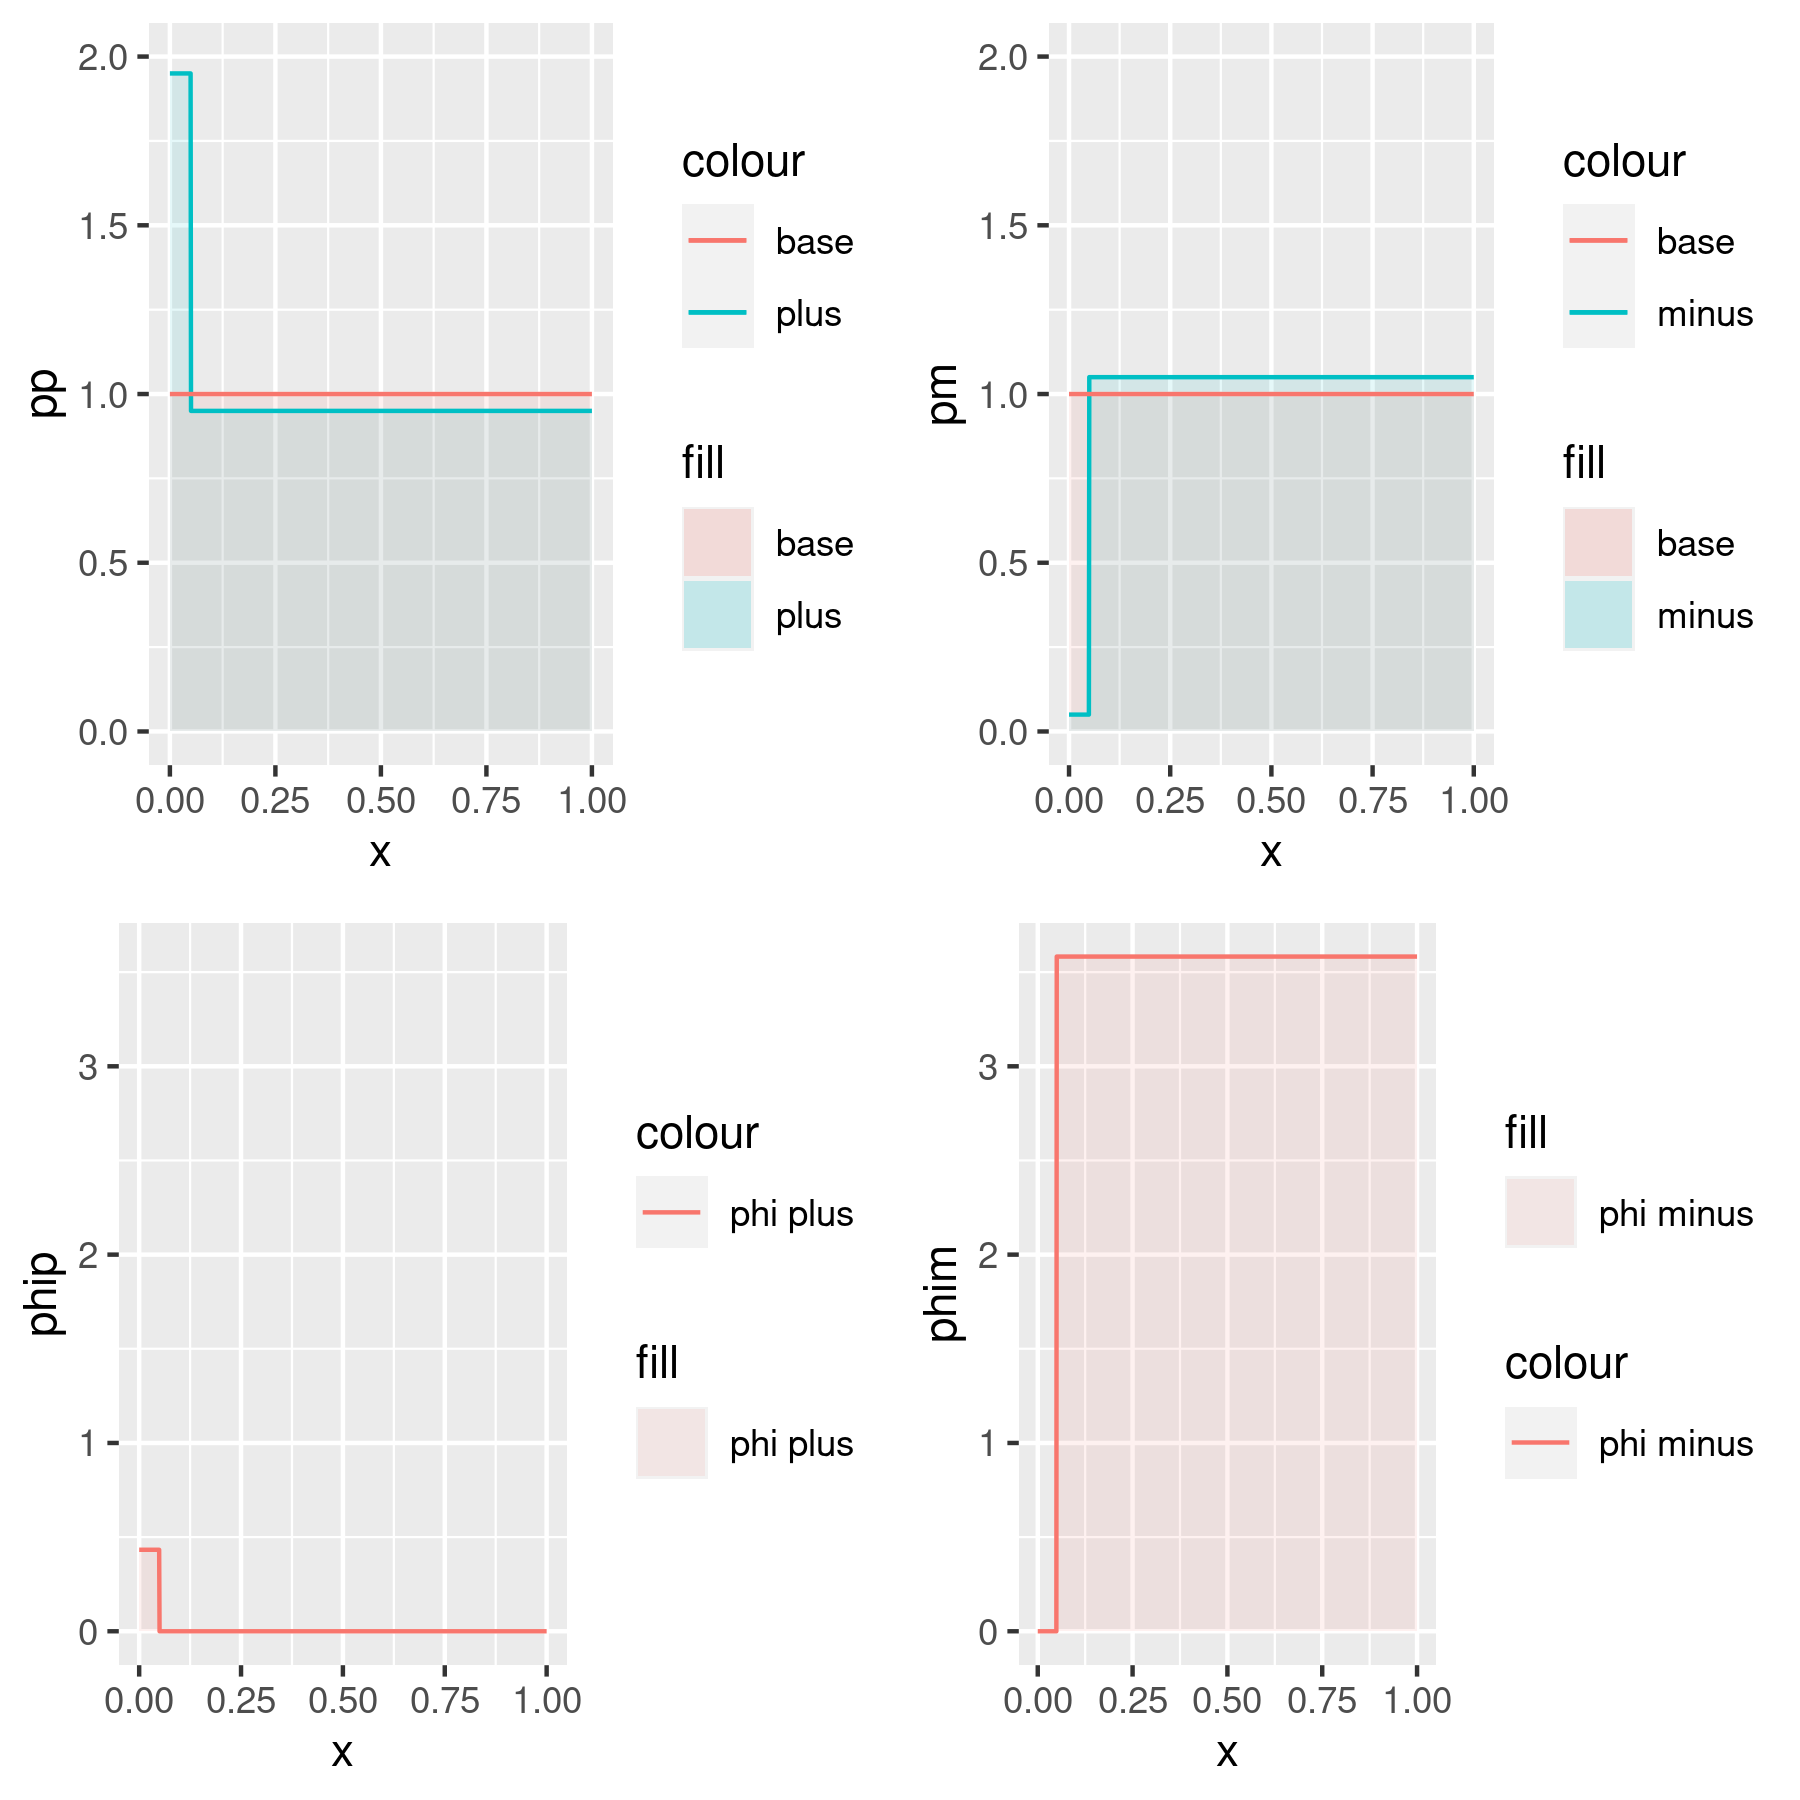
\includegraphics[width=0.980\linewidth,height=0.980\linewidth]{static_images/positive_phi_example.png}
% %
% \caption{A plot of the perturbations from \exref{positive_pert_large}
% with $p=2$ and $\epsilon=0.05$.  Positive $\phi$ can only add mass, so to remove
% a small amount of mass requires adding mass everywhere else and re-normalizing,
% resulting in a large perturbation according to $\norm{\cdot}_p$.}
% %
% \figlabel{positive_pert_large}
% \centering
% \end{figure}
%%%%%%%%%%%%%%%%%%%%%%%%%%%%%%%%%%%%%%%%%%%%%%%%%%%%%%%%%%%%%%%%%%%%%%%%%

Let $\pbase(\nu) = \ind{0 \le \nu \le 1}$.  For some $\delta > 0$ and $0 <
\epsilon \ll 1$, let
%
\begin{align*}
%
\palt(\nu) :={}&
    \left(\frac{1-\delta \epsilon}{1 - \epsilon} \right)
        \ind{\epsilon \le \nu \le 1} +
    \delta \ind{0 \le \nu \le \epsilon}.
%
\end{align*}
%
% where the final approximation is due to the smallness of $\epsilon$.
Then \eqref{phi_for_palt} gives, for some $\alpha$,
%
\begin{align*}
%
\phi ={}&
    \left( \alpha\left(\frac{1-\delta \epsilon}{1-\epsilon} \right)^{1/p}
        - 1
    \right)
        \ind{\epsilon \le \nu \le 1} +
    \left(\alpha \delta^{1/p} - 1 \right) \ind{0 \le \nu \le \epsilon}.
%
%
\end{align*}
%
And
%
\begin{align*}
%
\norm{\phi}_p ={}&
    \left( \alpha\left(\frac{1-\delta \epsilon}{1-\epsilon} \right)^{1/p} - 1
    \right) (1- \epsilon) +
    \left(\alpha \delta^{1/p} - 1 \right) \epsilon.
%
\end{align*}
%
For $\phi$ to be positive, we require
%
\begin{align*}
%
\alpha^p \ge \frac{1 - \epsilon}{1 - \delta \epsilon}
    \mathtxt{and}
\alpha^p \ge \frac{1}{\delta}.
%
\end{align*}

First, let us consider adding a small amount of prior mass, taking $\delta = 2 -
\epsilon$; let the corresponding perturbation be $\phi^+$.  For $\delta > 1$,
then we achieve $\phi \ge 0$ by taking $\alpha^p = \frac{1 - \epsilon}{1 -
\delta \epsilon}$.  Using the fact that $\epsilon \ll 1$ and keeping only
leading-order terms,
%
\begin{align*}
%
\frac{1-\epsilon}{1 - \delta \epsilon} \approx{}&
    (1- \epsilon)(1 + \delta \epsilon)
\\\approx{}& 1 + (\delta - 1) \epsilon
\\\approx{}& 1 + \epsilon,
%
\end{align*}
%
so
%
\begin{align*}
%
\norm{\phi^+}_p  ={}&
    \left(\alpha \delta^{1/p} - 1 \right) \epsilon
\\\approx{}&
    \left(
        \left( \left(1 + \epsilon\right) \left(2 - \epsilon \right)\right)^{1/p}
        - 1 \right) \epsilon
\\\approx{}&
%
\left( 2^{1/p} - 1 \right) \epsilon.
%
\end{align*}
%

Next, consider removing the same amount of mass with the symmetric change
$\delta = \epsilon$, letting $\phi^-$ be the corresponding perturbation. Then we
can ensure that $\phi(\nu) \ge 0$ with $\alpha^p \ge \epsilon^{-1}$, and
$\epsilon \ll 1$ gives
%
\begin{align*}
%
\frac{1-\delta\epsilon}{1 - \epsilon} \approx{}& 1- \epsilon,
%
\end{align*}
%
and
%
\begin{align*}
%
\norm{\phi^-}_p  ={}&
    \left( \alpha\left(\frac{1-\delta \epsilon}{1-\epsilon} \right)^{1/p} - 1
    \right) (1- \epsilon)
\\\approx{}&
\left(\left(\frac{1- \epsilon}{\epsilon}  \right)^{1/p} - 1\right)(1 - \epsilon)
%
\\\approx{}&
    \left( \frac{1}{\epsilon}\right)^{1/p}.
%
\end{align*}

Since $\epsilon$ is small, $\norm{\phi^-}_p \approx \left(
\frac{1}{\epsilon}\right)^{1/p} \gg \norm{\phi^+}_p \approx \left( 2^{1/p} - 1
\right) \epsilon$, despite the two perturbations respectively removing and
adding the same amount of arbitrarily small probability mass.

\end{ex}
%%%%%%%%%%%%%%%%%%%%%%%%%%%%%%%%%%%%%%%%%%%%%%%%%%%%%%%%%%%%%%%%%%%%%%%%%


\section{Evaluating stick expectations}\applabel{gh_quadrature}
We describe how to compute expectations with repsect to the stick-breaking
proportion $\nu_\k$. Let $f: \mathbb{R}\mapsto\mathbb{R}$ be a smooth function,
and we are interested in expectations of the form
\begin{align*}
  \expect{\q(\nuk \vert \eta)}{f(\nuk)}.
\end{align*}
For example, $f$ might be $f(\nu_\k) = \log \pstick(\nu_\k)$, whose
expectation appears in the $\mathrm{KL}$ divergence.

Recall that we chose the distribution on the logit-transformed
stick-breaking proportions $\lnu_\k$ to be normally distributed.
Let $\lnumean_\k$ and $\lnusd_\k$ be the location and scale, respectively,
of the Gaussian distribution on $\lnu_\k$.
Also let $\s$ be the sigmoid function, so that $\nu_\k = \s(\lnu_\k)$.

To compute expectations of a smooth function
$f(\nuk)$, the law of the unconscious statistician states that,
\begin{align*}
  \expect{\q(\nuk \vert \eta)}{f(\nuk)} ={}&
  \expect{\q(\lnu_\k \vert \eta)}
         {f\circ \s\left(\lnu_\k\right)}.
\end{align*}
By choosing $\q(\lnu_\k \vert \eta)$ to be Gaussian,
the right-hand side of is a Gaussian integral,
which we approximate
using GH quadrature with $\ngh$ knots,
located at $\xi_g$, weighted by $\omega_g$:
%
\begin{align}\eqlabel{gh_integral}
%
\expect{\q(\lnu_\k \vert \eta)}
       {f\circ \s\left(\lnu_\k\right)}
\approx{}&
    \sum_{g=1}^{\ngh} \omega_g f\circ \s \left(\lnusd_\k \xi_{g} + \lnumean_\k\right)
 \nonumber\\=:{}&
\expecthat{\q(\nuk \vert \eta)}{f(\nuk)}.
%
\end{align}
%
Using GH quadrature to approximate the expectation
is similar to the ``reparameterization trick,'' only using
GH points rather than standard normal draws.


\section{Regression mixture model details}\applabel{app_mice}
\subsection{The data}
The data come from a publicly available data set of mice gene expression
\citep{shoemaker:2015:ultrasensitive}.
Our analysis focuses on mice treated with the ``A/California/04/2009'' strain.
We normalize the data as described in
\citet{shoemaker:2015:ultrasensitive} and then apply the differential
analysis tool EDGE \citep{Storey:2005:significance} to rank the genes from most to least significantly differentially expressed.
We run our analysis on the top $\ngenes = 1000$ genes.

\subsection{The B-spline basis}
Notice from \figref{example_genes}, which shows an example time-course for a single gene,
that the time points are unevenly spaced, with more frequent observations at the beginning.
Following \citet{Luan:2003:clustering} we use cubic B-splines to smooth the time course expression data.
Specifically, we model the first 11 time points using
cubic B-splines with 7 degrees of freedom.
For the last three time points, $\timeindx = 72, 120, 168$ hours,
we use indicator functions.
That is, if $\tilde \regmatrix$ is the design
matrix where each column is a
B-spline basis vector evaluated at the $\ntimepoints$ measurement times,
we append to $\tilde \regmatrix$ three additional columns:
in these columns, entries are 1
if $\timeindx = 72, 120,$ or 168, receptively, and 0 otherwise.
The resulting matrix is the full design matrix $\regmatrix$.
We use indicators for the last three time points for numerical stability;
without the indicator columns,
the matrix $\tilde \regmatrix^T \tilde \regmatrix$ is nearly singular
because the later time points are more spread out.
The left column of \figref{example_genes} shows our basis functions.

\subsection{The generative model}
\eqref{mice_model} gives the per-component conditional likelihood.
We use a normal prior for the shifts $\b_\n$,
a multivariate normal prior for the coefficients $\mu_\k$,
and a gamma prior for the inverse variance $\tau_\k$.
The prior on the mixture weights $\pi$ are constructed using the stick-breaking
construction in the main-text, and the cluster assignments $\z_\n$
are drawn from a multinomial with wieghts $\pi$, as usual.



\subsection{The variational approximation}
The variational approximation, factorizes as
\begin{align*}
\q(\zeta \vert \eta) =
    \left( \prod_{\k=1}^{\kmax - 1} \q(\nuk \vert \eta) \right)
    \left( \prod_{\k=1}^{\kmax} \q(\beta_\k \vert \eta) \right)
    \left( \prod_{\n=1}^{\N} \q(\z_{\n} \vert \eta)
    \q(\b_{\n} \vert \z_{\n}, \eta)\right).
\end{align*}
Note that the variational distribution for $\b_\n$ conditions on $\z$.
We set $\q(\b_{\n} \vert \z_{\n} = k, \eta)$ to be Gaussian
with variational parameters dependent on $\k$.
For simplicity in this application,
we let $\q(\beta_\k \vert \eta) = \delta (\beta_k \vert \eta)$,
where $\delta(\cdot \vert \eta)$ denotes a point mass at a parameterized location.

As discussed in \exref{qz_optimality},
the optimal distribution $\q(\z_\n\vert\eta)$ is multinomial whose parameters
can be set in closed form as a function of the global variational parameters only.
We allow the distribution of $\b_\n$ to depend on $\z_{\n\k}$ so that
the its optimal distribution can also be set in closed form as a function of
global parameters.

The optimal distribution $q(\b_\n\vert \z_{\n\k} = 1, \eta)$ is Gaussian,
\begin{align*}
q(\b_\n\vert \z_{\n\k} = 1, \eta) = \normdist{\b_\n \vert \hat\mu_{\b_{\n\k}}, \hat\sigma^2_{\b_{\n\k}}}.
\end{align*}
Let
\begin{align*}
  \rho^{(1)}_{\n\k} &= \expect{\q(\beta_k|\eta)}{\sum_{m=1}^\ntimepoints \tau_{k}(x_{nm} - \regmatrix_m\mu_\k)} +
  \tau_0 \mu_0 \\
  \rho^{(2)}_{\n\k} &= \ntimepoints \expect{\q(\beta_k|\eta)}{\tau_{k}} + \tau_0,
\end{align*}
where $\mu_0$ and $\tau_0$ are the prior mean and information on $\b_n$, respectively.

The optimal parameters for the Gaussian distribution on $\b_\n$ is given by
\begin{align*}
  \hat\mu_{\b_{\n\k}} &= \rho^{(1)}_{\n\k} / \rho^{(2)}_{\n\k}\\
  \hat\sigma^2_{\b_{\n\k}} &= 1 / \rho^{(2)}_{\n\k}.
\end{align*}

\figref{gene_centroids} shows the inferred smoothers
$\regmatrix \expect{\q}{\mu_\k}$ for selected clusters. 
\MiceSmoothers

% with parameters $\hat\mu_{\b_{\n\k}}, \hat\mu_{\b_{\n\k}}:


\section{fastSTRUCTURE model details}\applabel{app_structure}
The generative process was described in the main text (\secref{results_structure}).
We detail here the variational approximation.
Like in all our examples, the variational distribution is mean-field:
\begin{align*}
\q(\zeta \vert \eta) =
    \left(
    \prod_{\n=1}^{\nindiv}\prod_{\k=1}^{\kmax - 1}
    \q(\nu_{nk} \vert \eta) \right)
    \left(\prod_{\k=1}^{\kmax}\prod_{l=1}^{\nloci}
    \q(\latentpop_{\k l} \vert \eta) \right)
    \left( \prod_{\n=1}^{\N} \prod_{l=1}^{\nloci} \prod_{i=1}^{2} \q(\z_{\n l i} \vert \eta) \right).
\end{align*}
We let all distributions be conditionally conjugate except for the sticks,
which are logit-normal.
Each membership indicator $\z_{\n l i}$ is categorical, and the
allele frequencies $\latentpop_{\k l}$ are Dirichlet distributed.

In this model, we still call $(\beta, \nu)$ the global latent variables, even though they scale
with the number of individuals $\N$;
they do not, however, scale with both the number of individuals and the number of loci
like $\z$ does. Thus, we call $\z$ the local latent variables.
The local variational parameters $\eta_\z$ can be set optimally in
an analagous way as \exref{qz_optimality}, except with the
indices $\n\k$ replaced with $\n\l\i\k$.


\section{fastSTRUCTURE supplemental results}\applabel{app_structure_results}
Recall from \secref{results_structure} and \figref{stru_func_sens_admix}
that the linear approximation
failed to capture the change in the admixture proportion of an individual,
$n = 25$ after a worst-case functional perturbation.

\figref{stru_lin_bad_example} examines individual $n = 25$ more closely.
The bottom row plots this individual's
admixture proportions as $\t$ varies from 0 to 1 in the perturbed prior
$\p(\nu\vert \t) = \p_0(\nuk)\exp(\t\phiworstcase(\nuk))$.
The linearized parameters poorly captured the change in admixture proportions observed after refitting, particularly
for populations 1 and 2, for values of $\t$ close to 1.
Even though we retain non-linearities
in the mapping from variational parameters to the posterior statistic,
for this perturbation, the mapping from prior parameter
$\t$ to the relevant variational parameters
is highly non-linear.
This latter mapping is what we linearize
and what causes our approximation to fail in this case.
Specifically, the variational location parameter on the first stick-breaking proportion is concave as a function of $\t$ ---
the location parameter increases for small $\t$,
then decreases as $\t\rightarrow1$.
However,
$\etalin(\t)$ linearizes the relationship between the location parameter and $\t$.
Therefore, the corresponding admixture mixture proportion of
population 1 is over-estimated under the linearized variational parameters.
Furthermore, because our linearized variational parameters
over-estimated the length of the first stick,
and the second admixture proportion is a product of the
remaining stick times the second stick-breaking proportion,
the linearized variational parameters then under-estimates
the admixture proportion of population 2.

\StructureLimitationsA

\figref{stru_fully_lin_example} shows a similar situation for individual $n = 74$.
The linearized variational parameters grossly over-estimated the length of the first stick,
resulting in the later admixture proportions being under-estimated.
The third admixture proportion was particularly poorly approximated under the linearized variational parameters.
Given the recursive nature of the relationship between admixtures and stick-breaking proportions, errors at early sticks affect later admixture proportions.
Fully linearizing the mapping $\t\mapsto\g(\etaopt(\t))$ to form the approximation
$\glin(t)$ avoids this problem.
In this example, $\glin(t)$ outperforms $\g(\etalin(t))$, with $\g$ being the admixture proportion of population 3.
In our experience,
computing $\g(\etalin(t))$, and thus retaining non-linearities in the mapping from $\eta\mapsto\g(\eta)$,
is usually beneficial to the quality of the approximation.
It is likely that $\g(\etalin(t))$ outperforms $\glin(\t)$ for most posterior quantities,
though as we see in \figref{stru_fully_lin_example},
this is not guaranteed to always be true.

\StructureLimitationsB


% I'm not sure where VB details are going to go, but Bryan, whenever you add
% the right section, just update the other reference to point to your new
% sections.
\section{Unconstrained variational parameterizations}
\applabel{app_vb_details}
Recall from \thmref{etat_deriv} that we require the optimal variational parameters
$\etaopt$ to be in the interior of its domain. One way to achieve this
is to use only \textit{unconstrained} parameterizations for the
component distributions of $\q$. One such parameterization was
presented in \exref{qz_optimality}, where we let
$\eta_{\z_\n}$, which parameterize the cluster assignments, be allowed to
take any value in $\mathbb{R}^{\kmax - 1}$; the assignment probabilities
$m_{\n}\in\mathbb{R}^{\kmax}$, which are constrained to sum to one,
are then formed with an appropriate transform of the unconstrained parameters
$\eta_{\z_\n}$

Other variables require careful parameterization as well.
For instance, instead of parameterizing the normal distribution on
logit-sticks $\lnu_\k$ using a mean and variance, we let $\eta_{\nu_\k}\in\mathbb{R}^2$
be the mean and \textit{log} variance. The variance is constrained to be positive;
the log-variance is unconstrained on the real line.
In general, a real-valued parameter $\mu_i$ which must be constrained
$a \leq \mu_i \leq b$ can be transformed to its unconstrained parameterization
by letting
\begin{align*}
  \eta_i = \log(\mu_i - a) - \log(b - \mu_i).
\end{align*}

In the variational approximation to the GMM model,
we let the component variables $\beta_\k$ be Normal-Wishart.
In this case, the scale matrix of the Normal-Wishart, $W_\k\in\mathbb{R}^{d\times d}$,
is constrained be positive definite.
Because $W$ is symmetric, we only neeed $d(d + 1) / 2$ parameters to represent it.
To form an unconstrained parameterization, we factorize $W$ using the Cholesky decomposition,
\begin{align*}
W = L^T L,
\end{align*}
where $L$ is a lower-triangular matrix, with positive diagonal entries.
The unconstrained parameterization of $W$ is then taken to be
the strictly lower-diagonal entries of $L$,
along with the $\log$ of the diagonal entries of $L$.




\end{document}
